% !TEX encoding = UTF-8 Unicode
\documentclass[a4paper]{article}

\usepackage{color}
\usepackage[obeyspaces]{url}
\usepackage[T1]{fontenc} % enable Cyrillic fonts
\usepackage[utf8]{inputenc} % make weird characters work
\usepackage{graphicx}
% \usepackage[margin=1.5in]{geometry}
\usepackage[table]{xcolor}
\usepackage{tocloft}
\usepackage{float}
\addtolength{\cftsecnumwidth}{10pt}

\usepackage[english,serbian]{babel}
%\usepackage[english,serbianc]{babel} 

\PassOptionsToPackage{obeyspaces}{url}
\usepackage[unicode]{hyperref}
\hypersetup{colorlinks,citecolor=green,filecolor=green,linkcolor=blue,urlcolor=blue}

\usepackage{listings}
\renewcommand\lstlistingname{Kod}
\renewcommand\lstlistlistingname{Kodovi}

\definecolor{mygreen}{rgb}{0,0.6,0}
\definecolor{mygray}{rgb}{0.5,0.5,0.5}
\definecolor{mymauve}{rgb}{0.58,0,0.82}

\lstset{
  backgroundcolor=\color{white},   % choose the background color; you must add \usepackage{color} or \usepackage{xcolor}; should come as last argument
  basicstyle=\scriptsize\ttfamily,        % the size of the fonts that are used for the code
  breakatwhitespace=false,         % sets if automatic breaks should only happen at whitespace
  breaklines=true,                 % sets automatic line breaking
  captionpos=b,                    % sets the caption-position to bottom
  commentstyle=\color{mygreen},    % comment style
  deletekeywords={...},            % if you want to delete keywords from the given language
  escapeinside={\%*}{*)},          % if you want to add LaTeX within your code
  extendedchars=true,              % lets you use non-ASCII characters; for 8-bits encodings only, does not work with UTF-8
  firstnumber=1,                   % start line enumeration with line 1000
  frame=single,	                   % adds a frame around the code
  keepspaces=true,                 % keeps spaces in text, useful for keeping indentation of code (possibly needs columns=flexible)
  keywordstyle=\color{blue},       % keyword style
  language=Python,                 % the language of the code
  morekeywords={*,...},            % if you want to add more keywords to the set
  numbers=left,                    % where to put the line-numbers; possible values are (none, left, right)
  numbersep=5pt,                   % how far the line-numbers are from the code
  numberstyle=\tiny\color{mygray}, % the style that is used for the line-numbers
  rulecolor=\color{black},         % if not set, the frame-color may be changed on line-breaks within not-black text (e.g. comments (green here))
  showspaces=false,                % show spaces everywhere adding particular underscores; it overrides 'showstringspaces'
  showstringspaces=false,          % underline spaces within strings only
  showtabs=false,                  % show tabs within strings adding particular underscores
  stepnumber=2,                    % the step between two line-numbers. If it's 1, each line will be numbered
  stringstyle=\color{mymauve},     % string literal style
  tabsize=2,	                     % sets default tabsize to 2 spaces
  title=\lstname                   % show the filename of files included with \lstinputlisting; also try caption instead of title
}

\begin{document}

\title{[RS] Skripta: Pitanja i odgovori}

\author{Momir Adžemović}

\date{1.~april 2020.}

\maketitle

\tableofcontents

\section{Koji od pokazivača p1, p2 i p3 nije ispravno definisan u primeru?}
		 \begin{lstlisting}
			int* p1,p2;
			int* p3=(int*)1000;\end{lstlisting}
		Pokazivač p2 nije ispavno definisan tj. p2 je običan ceo broj.

\section{U kakvom su odnosu dužine nizova s1 i s2 u primeru:}
		\begin{lstlisting}
			char s1[] = "C++";
      char s2[] = {'C', '+', '+' };\end{lstlisting}
      $sizeof(s1) == 4$\\
      $sizeof(s2) == 3$
    
\section{Šta će ispisati ovaj program?}
    \begin{lstlisting}
      int a = 1;
      int* b=&a;
      main(){
        *b = a + 1;
        *b = a + 1;
        cout << a << endl;
      }\end{lstlisting}

    Ispisaće 3.

\section{Koji koncepti programskog jezika C++ se upotrebljavaju da bi se 
         povećala (potencijalno ponovljena) upotrebljivost napisanog koda?}
    Polimorfizam, nasleđivanje, virtualno nasleđivanje, šabloni.

\section{Koji je redosled uništavanja objekata u primeru:}
    \begin{lstlisting}
    int a(3);
    main() {
      int* n = new int(10);
      int k(3);
      ...
      delete n;
    }\end{lstlisting}
    Napomena! Tip $int$ je primitivni tip, ne objekat. Ako bi promenljiva $a$ predstavljala objekat, 
    onda bi redosled uništavanja bio sledeći: Prvo će se unistiti $n$, pa $k$, i na kraju $a$.

\section{Da li je neka (koja?) narednih linija neispravna?}
    \begin{lstlisting}
    short* p = new short;
    short* p = new short[900];
    short* p = new short(900);
    short** p = new short[900];\end{lstlisting}

    $short** p = new short[900];$ će da vrati grešku pri kompiliranju, jer se ne poklapaju tipovi, 
    $p$ je $short**$ i pokušavamo da mu dodelimo nešto što je $short*$.
    \textbf{“error: cannot convert ‘short int*’ to ‘short int**’ in initialization”}
 
\section{Koje operacije klase Lista se izvršavaju u sledećoj naredbi:}
  \begin{lstlisting}
  Lista l2 = Lista();\end{lstlisting}

    \begin{enumerate}
      \item alocira se memorija za objekat Lista;
      \item poziva se eksplicitan konstruktor za objekat Lista;
    \end{enumerate}
    \thinspace
    \begin{itemize}
      \item Zašto se ne poziva operator dodele?
      \item Zašto se ne poziva konstruktor kopije? \cite{gfg_copy_assignment}
            \cite{cppref_copy_assignment}
      \item \textbf{the rule of three} \cite{sof_rule_of_three}
    \end{itemize}
    
\section{Koliko puta se poziva destruktor klase A u sledećem programu?}
    \begin{lstlisting}
    main() {
      A a, b;
      A& c = a;
      A* p = new A();
      A* q = &b;
    }\end{lstlisting}

    Tri puta. Pri deklaracija promenljivih $a$, $b$ i $p$. Promenljive $c$ i $q$ su reference 
    na objekte.

\section{Šta su šabloni funkcija?}
    Šabloni funkcija predstavljaju specijalne funkcije koje rade sa generičkim tipovima. 
    Ukoliko nam je potrebno više verzija iste funkcije samo sa različitim tipom podataka ili klasa, 
    onda šablon funkcija može da zameni tu grupu funkcija. Takođe konstante mogu da budu generički 
    parametri. U suštini šabloni nam omogućavaju generičko programiranje. Šabloni predstavljaju tip 
    statičkog polimorfizma tj. polimorfizam koji se obrađuje tokom kompilacije.\cite{cppref_templates}

\section{Kako se pišu i koriste šabloni funkcija?}
  \noindent Primer:
  \begin{lstlisting}
    template<typename T> 
    T sum(T a, T b)
    {
      return a + b;
    }\end{lstlisting}
  \textbf{Napomena:} Ako napišemo šablon funkcije i ne koristimo u programu nijednom konkretnu funkciju,
  onda će nam kompajler dati isti izvršni kod kao da nismo pisali šablon. Kompajler prevodi 
  sve konkretizovane funkcije nekog šablona. Isto važi i za klase. \\
  \textbf{Napomena:} Ako definišemo konkretnu funkciju (npr. int sum(int a, int b)), onda on ima 
  prioritet u odnosu na šablon i ona će biti pozvana.

\section{Napisati šablon funkcije koja računa srednju vrednost dva broja za bilo koji numerički tip.}
\begin{lstlisting}
  template< typename T {
    T avg( T x, T y ){
    return (x+y)/2;
  }\end{lstlisting}

\section{Šta su šabloni klasa?}
  \noindent Primer:
  \begin{lstlisting}
    template<typename A, typename B>
    struct Pair{
      A first;
      B second;
    
      Pair(A f, B s)
        : first(f), second(s)
        {}
    }\end{lstlisting}
  Isto kao i šabloni funkcija, samo se odnosi na generičke klase. Primeri generičkih klasu su mape, 
  vektori, skupovi, \dots, koji su već deo C++-a. \\
  \indent Primer: ,,vector<int>``, možemo posmatrati kao funkciju 
  koja prima kao argument celobrojni tip i vraća vektor celih brojeva (konkretan vektor).

\section{Kako se prevode šabloni klasa?}
  Svi generički tipovi se zamene sa konkretnim tipovima.
  Primer: Za prethodno pitanje ,,vector<int>`` dobijamo tako što zamenimo sva pojavljivanja generičkog 
  tipa ,,T`` sa konkretnim tipom ,,int``. Dobijeni kod kompilator može prevesti na klasičan način. 
  Bitno je naglasiti da je ovaj proces statičan.

\section{Šta je neophodan uslov da bi se pozivi nekog metoda dinamički vezivali? Šta je dovoljan uslov?}
  \textbf{Napomena:} Mora da važi svaki \underline{neophodan uslov} i 
  mora da važi barem jedan \underline{dovoljan uslov}!\\
  \textbf{Neophodan uslov:} Metod mora biti virtuelan. Metod je virtuelan ako ima ključnu reč ,,virtual``.\\
  \textbf{Dovoljan uslov:} Objektu pristupimo preko reference ili preko pokazivača.
  Primer:
  \begin{lstlisting}
  object o1 = Object();
  o1.method(); // nije dinamicki

  object *o2 = new Object();
  o2->method() // jeste dinamicki, ako je virtualan metod

  object &o3 = o1;
  o3.mehtod() // jeste dinamicki ako je virtualan metod\end{lstlisting}
\section{Šta je virtualna funkcija?}
  Virtuelnce funkcije (virtuelne metode) su metode neke klase koje uz sebe imaju ključnu reč ,,virtual``.
  U C++-u podrazumevano povezivanje je statičko. Ako želimo da koristimo dinamički polimorfizam, potrebno je
  naglasiti to ključnom reči ,,virtual`` i pozivati taj metod preko pokazivača ili reference na objekat.\\
  \indent U Java-i su sve nestatičke metode implicitno virtuelne što donosi neke svoje olakšice. Mana 
  toga je efikasnost.

\section{Šta je čisto virtuelna funkcija?}
  U C++-u čisto virtuelna funkcija i apstraktna funkcija predstavljaju sinonime. Čisto virtuelna funkcija
  je funkcija koja nema svoju implementaciju u okviru klase. Klasa koja sadrži čisto virtuelnu funkciju
  je apstrakna klasa. Čisto virtuelnu metodu označavamo sa ,,$= 0$`` kao sufiks.
  Primer:
  \begin{lstlisting}
  class VirtualObject{
    public:
    VirtualObject() {}
    virtual void doSomething() = 0;
  }\end{lstlisting}

\section{Šta je apstraktna klasa?}
  Apstraktna klasa je klasa koja ima barem jednu čisto virtuelnu metodu. Apstraktna klasa ne može da
  ima svoju instancu, ali možemo imati pokazivač ili referencu na objekat apstrakne klase što nam
  omogućava da koristimo dinamički polimorfizam. Apstraktna klasa i dalje može da ima svoj konstruktor
  koji se poziva samo u okviru konstruktora klasa koje je nasleđuju.

\section{Šta su umetnute (inline) funkcije? Kako se pišu?}
  Umetnute ,,inline`` funkcije su funkcije koje imaju prefiks ,,inline``. Predstavlja sugestiju kompajleru
  da ,,proširi`` funkciju na mestu gde je pozvana. Ideja je da se zaobiđe postavljanje funkcije
  na ,,stackframe`` i da se povećaju performanse. \\
  \indent Ovo predstavlja samo sugestiju. Kompajler odlučuje da će li funkcija zapravo biti proširena. 
  Funkcije koje nemaju ,,inline`` takođe mogu biti proširene.

\section{Šta su umetnuti (inline) metodi? Kako se pišu?}
  Isto kao ,,inline`` funkcije.
  
\section{Koja su osnovna merila neuspeha pri razvoju softvera? Objasniti svaku ukratko.}
  Osnovno merilo neuspeha je izgubljena materijalna vrednost tj. plaćena cena neuspeha. Ovo se
  može reći i za projekte koji nisu nužno vezani za softver. \\
  \textbf{Merila neuspeha:}
  \begin{itemize}
    \item uložena sredstva 
    \item izgubljeno vreme 
    \item posledice po čitav poslovni sistem 
  \end{itemize}

\section{Koje su osnovne vrste neuspeha pri razvoju softvera? Objasniti svaku ukratko.}
  \begin{itemize}
    \item Prekoračenje troškova (potrošeni resursi);
    \item Prekoračenje vremenskih rokova:
          \begin{itemize}
            \item Troškovi zbog produženog razvoja;
            \item Troškovi zbog kašnjenja puštanja u rad;
          \end{itemize}
    \item Rezultat nije upotrebljiv:
          \begin{itemize}
            \item Sistem je implementiran u skladu sa zahtevima, ali ne odgovara stvarnim potrebama;
            \item Neispunjenost nefunkcionalnih zahteva;
          \end{itemize}
    \item Odustajanje od projekta (usled nekog od prethodno navedenih razloga (ili više njih);
    \item Katastrofalne greške (bagovi).
  \end{itemize}

\section{Šta je neupotrebljiv rezultat? Koji su aspekti neupotrebljivosti? Objasniti.}
  Sistem je uspešno implementiran po zadatim zahtevima, ali nije upotrebljiv ili se ne isplati
  koristiti ga.\\
  \textbf{Aspekti neupotrebljivosti:}
  \begin{itemize}
    \item \textbf{Neupotrebljiv korisnički interfejs:}
    \begin{itemize}
      \item Loše rešeni ergonomski uslovi (odnosi se na komfort i efikasnost);
      \item Nepostojanje fizičkog (hardverskog) odziva;
      \item Neintuitivan izgled korisničkog interfejsa;
      \item Problematične kontrole interfejsa;
      \item Spor odziv;
      \item Nepouzdanost.
    \end{itemize}
    \item \textbf{Procedura korišćenja nije ostvariva/dobra u realnim uslovima:}
    \begin{itemize}
      \item Uz kupljenu knjigu se dobija besplatna sveska, ali to mora da se zavede kao prodaja. 
            Ako sistem neomogućava promenu cene, to neće biti moguće. 
            Ako sistem ne dopušta da se cena manuelno postavi na 0, takode neće biti moguće.
      \item Pretraživanje knjiga (ili slicnog kataloga) koje podrazumeva unosenje tacnog naslova.
      \item Ako IS omogućava upravi da tacno vidi i kritikuje magacionare zbog neracionalnog zauzeca 
            prostora, a ne omogućava automatsku podrsku u vidu saveta, 
            magacioneri pocinju da trose nesrazmerno mnogo vremena za planiranje prostora. 
            Iako rezultat jeste mnogo bolja iskoriscenost prostora, 
            gubi se na vecem utrošku radnog vremena.
    \end{itemize}
  \end{itemize}

\section{Koji su najčesci uzroci neupotrebljivosti rezultata razvoja softvera? Objasniti ukratko.}
  \begin{itemize}
    \item Nerealni ili nejasni ciljevi projekta.
    \item Neprecizna procena potrebnih resursa.
    \item Loše definisani zahtevi: Komumanikacija sa klijentom u prvoj fazi je veoma bitna gde se
          razjašnjavaju svi detalji i postavljaju se sva neophodna pitanja.
    \item Slaba komunikacija između klijenta, razvijaoca i korisnika.
  \end{itemize}

\section{Na kojim stranama se nalaze problemi pri razvoju softvera? Objasniti ukratko i navesti 
         po jedan primer.}
    \begin{itemize}
      \item Problemi na strani klijenta;
      \item Problemi na strani razvijaoca;
      \item Višestrani problemi.
    \end{itemize}

\section{Koji su najcešci problemi na strani zainteresovanih lica (ulagača) pri razvoju softvera? 
         Objasniti ukratko.}
    \begin{itemize}
      \item Nerealni ili nejasni ciljevi projekta;
      \item Neusklađenost ciljeva i strategije;
      \item Politika ulagača;
      \item Komercijalni pritisak;
      \item Otpor korisnika prema primeni novog softvera.
    \end{itemize}

\section{Koji su najcešci problemi na strani razvijaoca pri razvoju softvera? Objasniti ukratko.}
    \begin{itemize}
      \item Slabo vođenje projekta;
      \item Neprecizna procena potrebnih resursa;
      \item Slabo izveštavanje o stanju projekta;
      \item Neupravljani rizici;
      \item Upotreba ,,nezrelih`` tehnologija;
      \item Nesposobnost da se iznese složenost projekta;
      \item Tok praktičnog razvoja bez cvrstih principa i pravila.
    \end{itemize}

\section{Koji su najčešci problemi koji se odnose na obe strane u razvoju softvera 
         (ulagači i razvijaoci)? Objasniti ukratko.}
    \begin{itemize}
      \item Slaba komunikacija između klijenata, razvijaoca i korisnika;
      \item Nepoverenje između klijenata i razvijaoca;
      \item Loše definisani zahtevi.
    \end{itemize}

\section{Objasniti kako pristupi planiranju mogu dovesti do problema.}
    Loše planiranje je jedan od najčešćih uzroka neuspeha. Ima dva osnovna oblika:
    nedovoljno planiranje i preterano planiranje.\\
    \indent \textbf{Nedovoljno planiranje} se obično ogleda kroz nedovoljnu analizu problema
    i/ili loše definisane zahteve i/ili neprecizno definisane zahteva. Najčešće posledice
    nedovoljnog planiranja su nesrazmerno veliki broj naknadnih korekcija zahteva,
    slaba upotrebljivost rešenja ili probijanje rokova.\\
    \indent \textbf{Preterano planiranje} se obično ogleda kroz preširoko i nekoncentrisano ulaženje 
    u projekat (suviše duboka i obimna analiza sa ranim detaljima) 
    i/ili preširoko ulaženje u implementaciju
    i/ili preambicioznost koja je nesrazmerna realnim mogućnostima. Najčešće posledice su
    kasno uočavanje propusta, otežana tranzicija i probijanje rokova. 

\section{Šta je upravljanje rizicima?}
      ,,Upravljanje rizicima je proces prepoznavanja, procenjivanja i kontrolisanja 
      svega onoga što bi u projektu moglo da krene naopako pre nego što 
      postane pretnja uspešnom dovršavanju projekta ili implementacije 
      informacionog sistema.``
  \\[5pt]
  \rightline{{\rm --- Whitten, 2001}}

  Ovo važi i za razvoj projekta koji nije nužno vezan za softver. Najveći značaj ima 
  dobro upravljenje rizicima u početnim fazama. Ovaj proces je otežan u slučaju dugačkih 
  razvojnih ciklusa.
 
\section{Koji su osnovni uzroci rizika u razvoju softvera? Navesti bar 7.}
  \begin{enumerate}
  \item manjak osoblja
  \item nerealni rokovi i budzet
  \item razvoj pogrešnih funkcija
  \item razvoj pogrešnog interfejsa
  \item preterivanje (,,pozlaćivanje``)
  \item neprekidni niz izmena u zahtevima
  \item slabosti eksterno realizovanih poslova
  \item slabosti u eksterno nabavljenim komponentama
  \item slabe performanse u realnom radu
  \item rad na granicama računarskih nauka
  \end{enumerate}

\section{Koji su najvažniji savremeni koncepti razvoja koji su nastali iz potrebe 
         za smanjivanjem rizika u razvojnom procesu?}
  \begin{itemize}
    \item Inkrementalni razvoj
    \item Određivanje koraka prema rokovima
    \item Pojačana komunikacija među subjektima
    \item U žizi su objekti a ne procesi
    \item Pravljenje prototipova
  \end{itemize}

\section{Objasniti princip inkrementalnog razvoja.}
  Umesto da se razvoj posmatra kao jedna velika celina, sa složenim projektom i implementacijom,
  ta celina se deli u niz inkrementalnih faza. Te faze se nazivaju \textbf{inkrementi ili ciklusi}. 
  Svaki inkrement ima sve osnovne podfaze, kao što su: analiza zahteva, dizajn, 
  implementacija i testiranje. \cite{guru99_incremental_model}\\
  \textbf{Dobit:}
  \begin{itemize}
    \item Svaka faza je manja i jednostavnija, čime je pojednostavljeno planiranje i implementacija.
    \item Veća tačnost planiranja troškova i rokova i tačnije izveštavanje o toku razvoja.
    \item Klijent može da odgovori na svaki napredak.
  \end{itemize}
  \textbf{Rizik:}
  \begin{itemize}
    \item Ako u prvim koracima zanemarimo predstojeće korake, onda postoji rizik da će
          u narednim koracima biti potrebne veće izmene.
    \item Ako se u prvim koracima uzmu u obzir svi prestojeći, onda postoji rizik da se 
          njihova složenost približi složenosti čitavog sitema (,,naduvavanje koraka``), 
          čime ovakav pristup gubi smisao.
    \item Često nije moguće sagledati unapred broj, cenu i ukupno trajanje svih koraka.
  \end{itemize}

\section{Objasniti princip određivanja koraka prema rokovima.}
  Za svaki inkrementalan korak se prvo odrede budžet i rokovi, a tek posle toga poslovi
  koji će tim korakom biti obuhvaćeni.\\
  \textbf{Dobit:}
  \begin{itemize}
    \item Drastično smanjivanje rizika od prekoračenja budžeta ili rokova;
    \item Uspostavljanje ritma redovnog isporučivanja novih verzija sistema;
    \item Redovnija kontrola kvaliteta i viši stepen poverenja između subjekta;
    \item Postepeno prilagođavanje korisnika novim elemetnima sistema.
  \end{itemize}
  \textbf{Mane:}
  \begin{itemize}
    \item Uspostavljanje tesnih okvira inkrementalnog koraka može otežati pojedine korake 
          i podići ukupnu cenu i trajanje razvoja;
    \item Neki elementi sistema se ne mogu prirodno podeliti u različite korake;
    \item Svaki korak zahteva troškove isporučivanja što u zbiru može da postane velika stavka u 
          slučaju velikog broja malih koraka;
    \item U prvim koracima se obično biraju poslovi koji donose vecu dobit;
    \item Pri kraju razvoja postoji rizik da se ne implementiraju poslovi ,,čija je cena 
          veca od dobiti`` iako su značajni za sistem kao celinu.
  \end{itemize}

\section{Objasniti princip pojačane komunikacije među subjektima.}
  U planiranju (i svakog pojedinačnog koraka) se uključuju u razmatranje 
  sve vrste subjekata u što većem broju.\\
  \textbf{Dobit:}
  \begin{itemize}
    \item Dobija se tačnija slika o potrebnim ciljevima iz različitih uglova;
    \item Smanjuje se rizik razvoja neupotrebljivog rešenja;
    \item Subjekti se kroz proces razvoja pripremaju za upotrebu.
  \end{itemize}
  \textbf{Mane:}
  \begin{itemize}
    \item Previše informacija može dovesti do preteranog planiranja, a time i do ,,naduvavanja`` 
          pojedinačnih koraka.
    \item Prevelikim razmatranjem mišljenja subjekta koji su navikli na postojeće procese i ne sagledavaju 
          planirane izmene može se smanjiti obim suštinskih funkcionalnih izmena u okviru koraka, a time i 
          nepotrebno povećati broj koraka da se dode do ,,konačnog`` rešenja.
  \end{itemize}

\section{Objasniti princip davanja prednosti objektima u odnosu na procese.}
  U središte pažnje se stavljaju objekti pre procesa. \\
  \textbf{Dobit:}
  \begin{itemize}
    \item Objekti su obično stabilniji od procesa (manje se menjaju i manje su šanse da se skroz obrišu);
    \item Prilagođeniju su inkrementalnom pristupu;
    \item Smanjuje se rizik od pogrešnih odluka u ranijim fazama razvoja (u ranijim fazama je više 
          akcenat na objektima, a na kasnijim na procesima). 
  \end{itemize}
  \textbf{Rizik:}
  \begin{itemize}
    \item Potpuno zanemarivanje procesa u ranim fazama može voditi ka pogrešnoj arhitekturi sistema
          što se kasnije teško menja;
    \item Sasvim detaljno razmatranje procesa u ranim koracima može da dovede do ,,naduvavanja`` koraka.
  \end{itemize}

\section{Objasniti princip pravljenja prototipova}
  U okviru analize problema se pravi prototip koji održava način funkcionisanja i upotrebe softvera.\\
  \textbf{Dobit:}
  \begin{itemize}
    \item Olakšava se netehničkim subjektima da u ranim fazama razvoja uoče određene nedostatke;
    \item Smanjuje se rizik od pogrešnih odluka u ranim fazama razvoja.
  \end{itemize}
  \textbf{Rizik:}
  \begin{itemize}
    \item Prototipovi obično odražavaju funkcionalne aspekte i elemente korisničkog interfejsa,   
          ali ne i unutrašnju strukturu softvera;
    \item Posledica je da su samo delemično odgovarajući objektno orijentisanim metodologijama;
    \item Nedovoljno široko napravljen prototip i nedovoljno široko razmatranje prototipa mogu da 
          prikriju nedostatke u drugim aspektima IS;
    \item Previše pažnje posvećene prototipu preti da ,,naduva`` fazu njegove izrade.
  \end{itemize}

\section{U kojim okolnostima su nastale objektno orijentisane razvojne metodologije?}
  \begin{enumerate}
    \item Postojanje metodologija koje strukturirano pristupaju analizi i opisivanju procesa;
    \item Potreba za strukturiranim opisivanjem podataka;
    \item Potreba za opisivanjem entiteta koji menjaju stanja;
    \item Podizanje nivoa apstraktnosti posmatranja elemenata sistema;
    \item Programiranje upravljano događajima;
    \item Vizuelni korisnički interfejsi;
    \item Povećana modularnost softvera;
    \item Skraćivanje razvojnog ciklusa;
    \item Tranzicija modela;
    \item Višestruka upotrebljivost softvera;
    \item i drugo \dots
  \end{enumerate}

  Za razliku od strukturnih, koje su u središte pažnje stavljale uređivanje procesa i algoritama, 
  objektno orijentisane metodologije u središte pažnje stavljaju uređivanje objekata kojima se opisuje 
  sistem. Razvoj objektno orijentisanih metodologija je počeo u vreme kada su slabosti prethodnih 
  metodologija bile uglavnom poznate. U njih su ugrađeni neki od predstavljenih savremenih koncepata 
  razvoja.

\section{Objasniti osnovne koncepte pristupanja objektno orijentisanih razvojnih metodologija 
         problemu razvoja.}
  \begin{itemize}
    \item U žižu se stavljaju objekti, a ne procesi;
    \item Sve objektno orijentisane metodologije se odlikuju skraćivanjem trajanja razvojnog ciklusa:
          \begin{itemize}
            \item RUP (i druge) propisuju inkrementalni razvoj,
            \item Agilne metodologije propisuju određivanje koraka prema rokovima i troškovima;
          \end{itemize}
    \item Pojačana komunikacija među subjektima u svim fazama.
  \end{itemize}


\section{Šta je objekat? Objasniti svojim rečima i navesti jednu od poznatih definicija.}
  ,,Objekti imaju stanje, ponašanje i identitet`` (Booch, 1994)\\\\
  Primer:
  \begin{lstlisting}
  class Point {
  private:
    int x, int y;
  public:
    Point(int _x, int _y)
      : x(_x), y(_y)
      {}

    void move(int dx, int dy)
    {
      x += dx;
      y += dy;
    }
  };

  int main()
  {
    Point point(2, 3);
    point.move(1, 4);
    return 0;
  }\end{lstlisting}
  Promenljiva ,,point`` predstavlja objekat klase ,,Point``. Njeno stanje je određeno
  atributima (poljima) ,,x`` i ,,y``. U ovom slučaju je stanje (x=2, y=3). Njeno ponašanje je 
  određeno metodom ,,move()`` tj. tačka može da se pomera. Njen identitet je ,,Point``.

\section{Šta je klasa? Atribut? Metod?}
  \begin{itemize}
    \item \textbf{Klasa} predstavlja skup objekata koji imaju isto ponašanje (isti skup metoda) 
          i isti skup atributa. 
    \item \textbf{Objekat} predstavlja konkretan primerak klase. Skup metoda opisuje ponašanje objekta. 
    \item \textbf{Metodi} su obično funkcije definisane u okviru neke klase. Atributi su polja klase 
          i preko njih tj. njihovih vrednosti se opisuje trenutno stanje objekta.
  \end{itemize}

\section{Koji su osnovni koncepti na kojima počivaju tehnike objektno orijentisanih metodologija?}
  \begin{itemize}
    \item enkapsulacija
    \item interfejs
    \item polimorfizam
    \item nasleđivanje: specijalizacija i generalizacija u hijearhiji klase. Smanjuje dupliran kod i
          koristi se za dinamički polimorfizam.
  \end{itemize}

\section{Objasniti koncept enkapsulacije.}
  Ideja je da se podaci i funkcije koje rade sa tim podacima spoje u jednu klasu. Klasa se deli
  na javni i privatni deo. Podaci se uglavnom nalaze u privatnom delu, sa izuzecima (javne statičke 
  konstante su relativno prihvatljive). Javne funkcije opisuju klasu i njenu svrhu u okviru modula
  u kojem se koristi.
  \begin{figure}[H]
    \begin{center}
        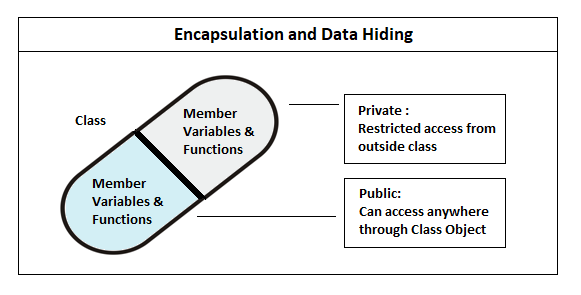
\includegraphics[width=80mm,height=50mm]{Slike/encapsulation.png}
    \end{center}
  \end{figure}
  Svrha je apstrahovanje strukture metodima i viši nivo međusobne nezavisnosti klasa od modula u
  kojem se upotrebljava.

\section{Objasniti koncept interfejsa.}
  Klasa je opisana korisniku preko javnih metodima klase (plavi, javni deo kapsule). Korisnik 
  interfejsa ne mora da zna implementaciju klase da bi je koristio. \\
  Svrha je sakrivanje složenosti implementacije. Suština objekta je u njegovom ponašanju.\\
  \textbf{Napomena:} Ako objekat ima više interfejsa, znači da ima više funkcija, pa je potrebno
  razmotriti njegovo razlaganje na više objekata.

\section{Objasniti koncept polimorfizma.}
  \noindent Poenta polimorfizma je da se jedan kod što više puta iskoristi. \\
  \textbf{Vrste:}
  \begin{itemize}
    \item hijearhijski (dinamički): dobijen kombinacijom dinamičkog povezivanja i nasleđivanja;
    \item parametarski (statički): šabloni;
    \item implicitni: retki jezici ovo podržavaju.
  \end{itemize}
  Pišemo apstrakniji kod koji ima veću upotrebljivost. \cite{catonmat_polymorphism}

\section{Objasniti koncept nasleđivanja  i odgovarajuće odnose.}
  Nasleđivanje klase je ekvivalentno uvođenju jednosmerne parcijalno uređene 
  relacije "jeste" između klasa.\\
  Klasa A ,,jeste`` klasa B akko svaki objekat klase A ima sve osobine koje imaju i objekti klase B.\\
  Ako A ,,jeste`` klasa B kaže se i da je:
  \begin{itemize}
    \item A ,,izvedena`` klasa iz B ili A ,,je potomak`` klase B
    \item B ,,osnovna`` klasa za A ili B ,,je predak`` klase A
  \end{itemize}
  Predstavlja osnovu za građenje hijerarhija klasa.\\
  Svrha:
  \begin{itemize}
    \item Nasleđivanje se koristi za eksplicitno označavanje sličnosti među klasama (objektima).
    \item Predstavlja osnovu za hijerarhijski polimor zam: ako se to može uraditi sa svakim objektnom klase B, 
          onda se to može uraditi i sa svakim objektom klase A koja je izvedena iz B.
  \end{itemize}
  Nasleđivanje se posmatra u dva smera, kao specijalizacija ili generalizacija:
  \begin{itemize}
    \item klasa A je poseban (specijalan) slučaj klase B
    \item klasa B je opstiji (generalan) slučaj klase A
  \end{itemize}

\section{Kroz koje faze je prošao razvoj OO metodologija?}
  \begin{itemize}
    \item Početni koraci (-1997)
    \item Oblikovanje UML-a (1995-2005)
    \item Post-UML koraci (2000-)
  \end{itemize}

\section{Koje su karakteristike prve faze razvoja OO metodologija?}
  \begin{itemize}
    \item Veliki broj različitih notacija i metodologija
    \item Nijedna kompletna i dovoljno široka
    \item Booch, 1991.
    \item Coad, Yourdon, 1991.
    \item Martin, Odell, 1992.
  \end{itemize}

\section{Koje su karakteristike druge faze razvoja OO metodologija?}
  \begin{itemize}
    \item Nekoliko dubljih metodologija koncetrisanih na različite faze razvoja
    \item Pokušaji ujednačavanja notacije
    \item Akcenat na notaciji
  \end{itemize}

\section{Koje su karakteristike treće faze razvoja OO metodologija?}
  \begin{itemize}
    \item Ujednačena notacija 
    \item Široko shvatanje procesa razvoja 
    \item Potpuno posvećenje metodologijama 
    \item RUP i druge savremene metodologije 
    \item Agilne metodologije
  \end{itemize}

\section{Šta je UML?}
  UML je \textbf{Objedinjeni jezik za modeliranje (Unified Modeling Language)}. 
  Oblikovan je paralelno uz metodologiju ,,Unified Approach`` (Objedinjeni pristup). Pretežno 
  grafički jezik (minimalno se koristi tekst van grafičkog prikaza). Olakšava vizuelizaciju 
  kompleksnog sistema i predstavlja tip dokumentacije. \cite{vp_uml}
  \begin{figure}[H]
    \begin{center}
        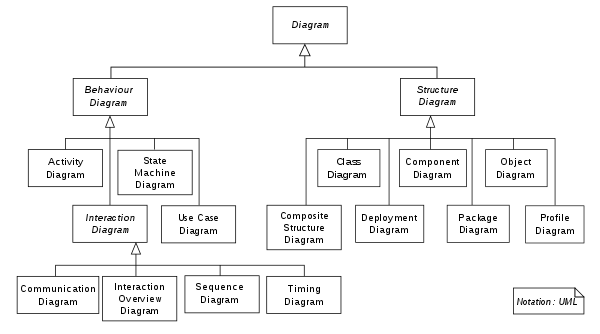
\includegraphics[width=100mm,height=70mm]{Slike/uml.png}
    \end{center}
  \end{figure} 


\section{Koje vrste dijagrama postoje u UML-u? Objasniti.}
  Dijagrami se dele u tri grupe:
  \begin{itemize}
    \item dijagrami ponašanja
    \item dijagrami interakcije (može se gledati i kao podgrupa dijagram ponašanja)
    \item strukturni dijagrami
  \end{itemize}

\section{Navesti strukturne dijagrame UML-a.}
  \begin{enumerate}
    \item Dijagram klasa (class diagram)
    \item Dijagram komponenti (component diagram)
    \item Dijagram objekta (object diagram)
    \item Dijagram profila (profile diagram)
    \item Dijagram složene strukture (composite structure diagram)
    \item Dijagram isporučivanja (deployment diagram)
    \item Dijagram paketa (package diagram)
  \end{enumerate}

\section{Koja je uloga i šta su osnovni elementi dijagrama klasa?}
  Ilustruje elemente statičkog modela tj. klase, njihov sadržaj i međusobne odnose.
  Klasa je predstavljena sa:
  \begin{itemize}
    \item nazivom
    \item atributima (ime, tip, vidljivost)
    \item metodama (ime, parametri, povratna vrednot, vidljivost)
  \end{itemize}
  Odnosi mogu biti:
  \begin{itemize}
    \item nasleđivanje (specijalizacija ili generalizacija)
    \item asocijacija:
          \begin{itemize}
            \item agregacija
            \item kompozicija
          \end{itemize}
    \item zavisnost (Neka je A zavisna od B. Ako se klasa B menja, onda klasa A može zahtevati promene,
          ali ne važi obrnuto)
  \end{itemize}
  \textbf{Kako razlikovati asocijaciju, agregaciju i kompoziciju?}\\
  Agregacija i kompozicija su specijalni slučajevi asocijacije. 
  Agregacija predstavlja odnos gde dete može da postoji bez roditelja (klase su čvorovi), 
  a kompozicija predstavlja odnos gde dete ne može da postoji bez roditelja.
  \begin{figure}[H]
    \begin{center}
        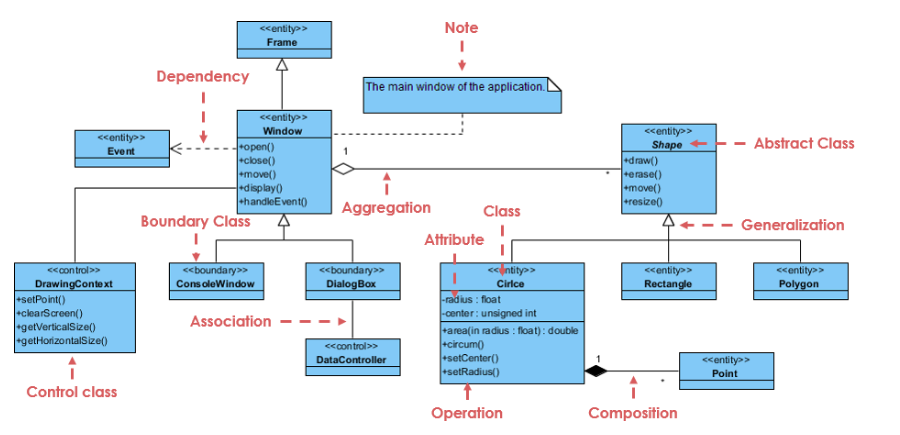
\includegraphics[width=120mm,height=75mm]{Slike/uml_klase.png}
    \end{center}
  \end{figure} 

\section{Koja je uloga i šta su osnovni elementi dijagrama komponenti?}
  Dijagram komponenti razbija sistem koji se razvija na neke celine po njihovim funkcionalnostima.
  Ima dosta sličnosti kao dijagram klase po odnosima elemenata. Ovaj dijagram možemo posmatrati
  kao apstraktniji nivo dijagrama klase. Svaki element ima naziv i interfejs.

\section{Koja je uloga i šta su osnovni elementi dijagrama objekata?}
  Ilustruje elemente dinamičkog modela tj. predstavlja objekte u jednom trenutku (konkretna situacija). 
  Koristi se kao dopuna dijagrama klase i komunikacije. Sastoji se od objekata (naziv klase i opis stanja)
  i njihovih odnosa.
  \begin{figure}[H]
    \begin{center}
        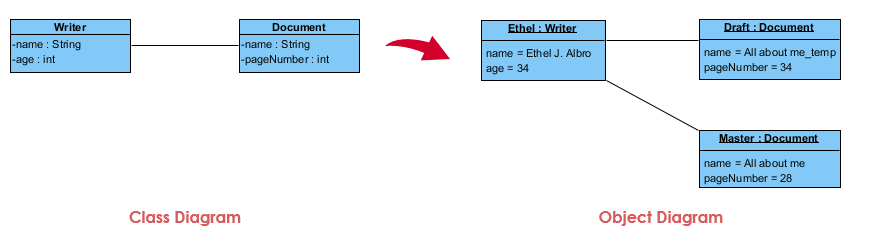
\includegraphics[width=120mm,height=50mm]{Slike/uml_objekat.png}
    \end{center}
  \end{figure} 

\section{Koja je uloga i šta su osnovni elementi dijagrama isporučivanja?}
  Predstavlja elemente fizičke arhitekture sistema. Ovo je nešto što bismo koristili 
  ako imamo distribuirani sistem gde imamo više servera. 
  Koriste se za planiranje arhitekture sistema. \\
  \textbf{Sadrži:}
  \begin{itemize} 
    \item čvorove (primer: server) 
    \item softverske ili hardverske podsisteme
    \item međusobne veze tih podsistema
    \item može da ilustruje zasupljenost komponenti u podsistemima.
  \end{itemize}

\section{Koja je uloga i šta su osnovni elementi dijagrama paketa?}
  Ilustruje kako su elementi logičkog modela organizovani u pakete, kao i međuzavisnosti paketa. 
  Paket je često sinonim za prostor imena (\textit{namespace}). Okuplja elemente koji su semantički 
  povezani i očekuje se da se zajedno menjaju. \\
  \textbf{Sadrži:}
  \begin{itemize}
    \item nazive i granice paketa
    \item klase u paketima
    \item međusobne odnose klasa
    \item međusobne zavisnosti paketa
    \item može se koristiti i u domenu slučajeva upotrebe
  \end{itemize}

\section{Navesti dijagrame ponašanja UML-a.}
  \begin{enumerate}
    \item Dijagram aktivnosti (activity diagram)
    \item Dijagram stanja (state machine diagram)
    \item Dijagram slučajeva upotrebe (use case diagram) 
          - u ove dijagrame se mogu ubrojati i dijagrami interakcije
  \end{enumerate}

\section{Koja je uloga i šta su osnovni elementi dijagrama aktivnosti?}
  Predstavlja poslovne procese višeg nivoa, tokove podataka i eventualno složene logičke elemente 
  sistema. Veoma sličan dijagramu za opisivanje algoritama. \\
  \textbf{Sadrži:}
  \begin{itemize}
    \item procese
    \item tokove podataka
    \item čvorove i grananja
    \item uslovne tačke
    \item početne i završne tacke
    \item može da sadrži i ,,linije autora``
  \end{itemize}
  \begin{figure}[H]
    \begin{center}
        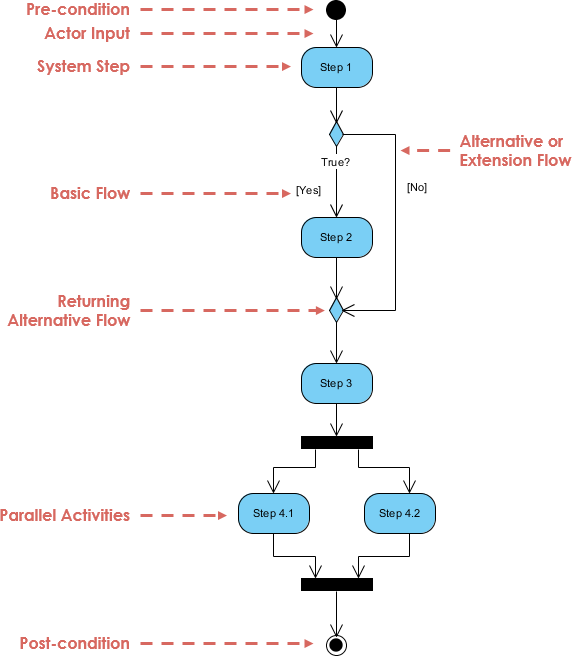
\includegraphics[width=80mm,height=80mm]{Slike/uml_aktivnost.png}
    \end{center}
  \end{figure}  

\section{Koja je uloga i šta su osnovni elementi dijagrama stanja?}
  Ovaj dijagram se koristi da se opišu ponašanja koja zavise od trenutnog stanja. Ovde smatramo
  da objekat reaguje drugačije na istu situaciju u zavisnosti od trenutnog stanja.\\ 
  \textbf{Sadrži:}
  \begin{itemize}
    \item sva moguća stanja objekta
    \item posebno označeno početno i završno stanje
    \item prelaske između stanja (događaji)
    \item strelica od prethodnog prema narednom stanju
    \item nazivi događaja koji menjaju stanje objekata
    \item odgovarajuća objašnjenja
  \end{itemize}
  \begin{figure}[H]
    \begin{center}
        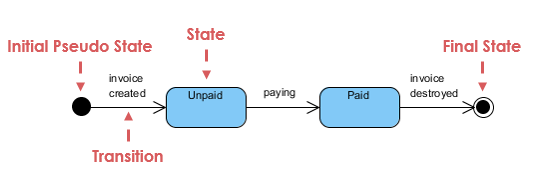
\includegraphics[width=80mm,height=40mm]{Slike/uml_stanja.png}
    \end{center}
  \end{figure} 

\section{Koja je uloga i šta su osnovni elementi dijagrama slučajeva upotrebe?}
  Predstavlja slučajeve upotrebe, aktere i njihove međusobne odnose. Ne prikazuje redosled
  po kojem se koraci izvršavaju.\\
  \textbf{Sadrži:}
  \begin{itemize}
    \item slučajeve upotrebe
    \item aktere
    \item pakete
    \item podsisteme
    \item međusobne odnose
  \end{itemize}
  \begin{figure}[H]
    \begin{center}
        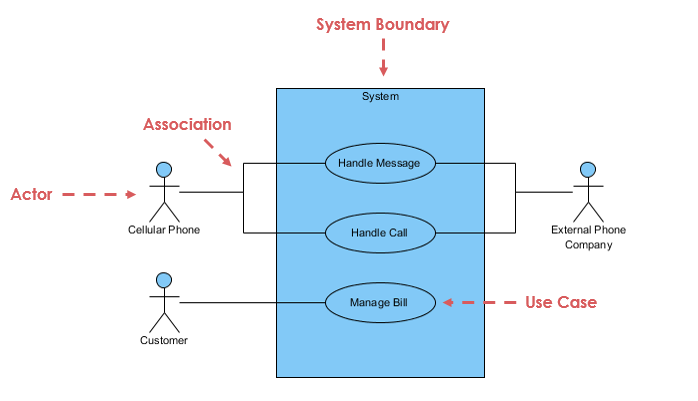
\includegraphics[width=100mm,height=60mm]{Slike/uml_slucaj_upotrebe.png}
    \end{center}
  \end{figure} 

\section{Navesti dijagrame interakcija.}
  \begin{enumerate}
    \item Dijagram komunikacije (communication diagram) 
          - raniji naziv, Dijagram saradnje (collaboration diagram)
    \item Dijagram interakcija (interaction diagram ili interaction overview diagram)
    \item Dijagram sekvence (sequence diagram)
    \item Dijagram vremena (timing diagram)
  \end{enumerate}

\section{Koja je uloga i šta su osnovni elementi dijagrama komunikacije?}
  Predstavlja produženje dijagrama objekata gde su predstavljene interakcije između objekata.
  Dijagram prikazuje objekte uz poruke koje oni šalju. Sadrži objekte, poruke i evetualno komentare.
  \begin{figure}[H]
    \begin{center}
        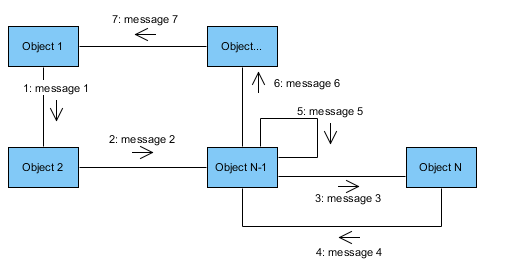
\includegraphics[width=100mm,height=60mm]{Slike/dijagram_komunikacije.png}
    \end{center}
  \end{figure} 

\section{Koja je uloga i šta su osnovni elementi dijagrama interakcije?}
  Predstavlja varijantu dijagrama aktivnosti gde su čvorovi interakcije ili aktivnost.\\
  \textbf{Sadrži:}
  \begin{itemize}
    \item objekte
    \item manje dijagrame aktivnosti ili interakcija
    \item slučajeve upotrebe
    \item tok odvijanja procesa (protoka podataka)
    \item grananja i spajanja
    \item početak i kraj
  \end{itemize}
  \begin{figure}[H]
    \begin{center}
        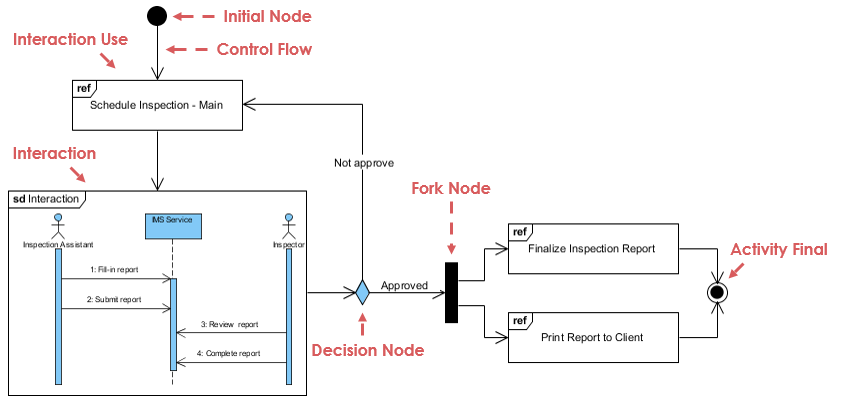
\includegraphics[width=120mm,height=60mm]{Slike/dijagram_interakcije.png}
    \end{center}
  \end{figure} 

\section{Koja je uloga i šta su osnovni elementi dijagrama sekvenci?}
  Prikazuju interakcije objekata u kontekstu saradnje. Ovi dijagrami imaju akcenat na vremenu i
  prikazuju redosled interakcija.\\
  \textbf{Sadrži:}
  \begin{itemize}
    \item aktere
    \item linije života (vreme)
    \item poruke poziva (započinu drugu liniju života)
    \item povratna poruka
    \item ostali tipovi poruka
  \end{itemize}
  \begin{figure}[H]
    \begin{center}
        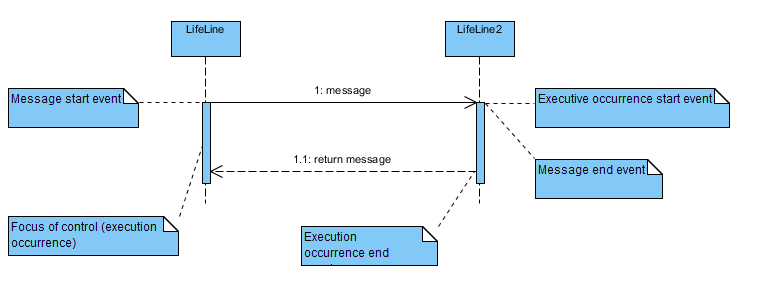
\includegraphics[width=100mm,height=60mm]{Slike/uml_sekvenci.png}
    \end{center}
  \end{figure} 

\section{Šta je uzorak za projektovanje? Čemu služi?}
  ,,Svaki uzorak za projektovanje opisuje problem koji se stalno ponavlja u našem okruženju i zatim
  opisuje suštinu rešenja problema tako da se to rešenje može upotrebiti milion puta, a da se
  dva puta ne ponovi na isti način.`` 
  \rightline{{\rm --- Cristopher Alexander}}\\

  Kristofer je ovde govorio za uzorke za zidanje zgrada, ali to što je rekao isto važi i za
  uzorke objektno orijentisanog projektovanja. Softverska rešenja su izražena pomoću objeta i 
  interfejsa umesto preko zidova i vrata, ali suština obe vrste uzoraka je rešavanje problema
  u svom kontektsu.\\
  \indent Uzorci za projektovanje su rešenja za opšte probleme sa kojim se razvijaoci često susreću.
  Ova rešenja su sakupljenja preko iskustava dobijenim na prethodnim lošim rešenjima koja su
  se javljala proteklih godina.\\
  \indent \textbf{Gang of four}: Erich Gamma, Richard Helm, Ralph Johnson i John Vlissides su objavili
  knjigu ,,Design Patterns: Elements of Reusable Object-Oriented Software``, što je započelo 
  koncepte o uzorcima projektovanja.

\section{Koji su osnovni elementi uzoraka za projektovanje? Objasniti ih.}
  Svaki uzorak ima četiri bitna elementa:
  \begin{itemize}
    \item Ime uzorka
    \item Problem
    \item Rešenje
    \item Posledice
  \end{itemize}

\section{Objasniti ime, kao element uzoraka za projektovanje.}
  U nekoliko reči opisuje, njegova rešenja i njegove posledice.
  Davanjem imena uzorku uvećava se rečnik projektovanja.
  Tako se projektovanje podiže na viši nivo apstrakcije.
  Rečnik uzoraka omogućava razmenu mišljenja o uzorcima, diskutovanje, pisanje i čitanje.
  Lakše je razmišljati o projektovanju i prenositi drugima taj model i njegove ocene.
  Pronalaženje dobrih imena je jedan od najtežih poslova pri izradi kataloga.

\section{Objasniti problem, kao element uzoraka za projektovanje.}
  Opisuje slučaj u kome se uzorak koristi.
  Opisuju se i problem i njegov kontekst.
  Moguć je opis specifičnih problema (primera).
  Problem može opisivati strukture klasa ili objekata čije osobine nagoveštavaju kruto 
  projektovanje. Ponekad problem sadrži spisak uslova potrebnih da bi se uzorak primenio.

\section{Objasniti rešenje, kao element uzoraka za projektovanje.}
  Opisuje elemente koji čine dizajn, njihove odnose, odgovornosti i saradnju.
  Ne opisuje određen konkretan projekat ili implementaciju, 
  pošto je uzorak kao šablon koji se može primeniti u mnogim različitim situacijama.
  Daje apstraktan opis problema projektovanja i uputstvo kako se on rešava opštim uređenjem 
  elemenata (klasa i objekata).

\section{Objasniti posledice, kao element uzoraka za projektovanje.}
  Obuhvataju rezultate i ocene primene uzorka.
  Često se ne pominju u opisima odluka o projektovanju, 
  ali su veoma bitne za procenu alternetiva i za razumevanje prednosti 
  i nedostataka primene uzorka.

\section{Navesti šta sve obuhvata opis jednog uzorka za projektovanje.}
  \begin{itemize}
    \item \textbf{Ime uzorka i klasifikacija:}
          \begin{itemize}
            \item Ime uzorka sažeto izlaže suštinu uzorka.
            \item Dobro ime je od suštinskog značaja pošto ono ulazi u rečnik projektovanja.
            \item Klasifikacija uzorka izvedena je po šemi koja će biti kasnije navedena.
          \end{itemize}
    \item \textbf{Namena:} Kratak iskaz koji odgovara na sledeča pitanja:
          \begin{itemize}
            \item Šta je uzrok a projektovanje radi?
            \item Kakvo mu je obrazloženje i namena?
            \item Na koje konkretno pitanje ili problem projektovanja se uzorak odnosi?
          \end{itemize}
    \item \textbf{Poznat takođe kao:} Ostala poznata imena uzorka (ako postoje).
    \item \textbf{Motivacija:}
          \begin{itemize}
            \item Scenario koji ilustruje problem projektovanja i način na koji strukture klasa 
                  i objekata u uzorku rešavaju taj problem.
            \item Scenario pomaže da se shvati apstraktniji opis uzorka.
          \end{itemize}
    \item \textbf{Primenljivost:}
          \begin{itemize}
            \item Na koje situacije se uzorak može primeniti?
            \item Koji su primeri lošeg projektovanja koje uzorak može da ispravi?
            \item Kako prepoznati te situacije?
          \end{itemize}
    \item \textbf{Struktura:} Grafički prikaz klasa u uzorku u notaciji UML 
          \begin{itemize}
            \item dijagrami klasa
            \item dijagrami interakcije
          \end{itemize}
    \item \textbf{Učesnici:} Klase i/ili objekti koji učestvuju u uzorku za projektovanje kao i njihove odgovornosti.
    \item \textbf{Saradnja:} Kako učesnici sarađuju da bi izvršavali svoje odgovornosti.
    \item \textbf{Posledice:}
          \begin{itemize}
            \item Kako uzorak zadovoljava svoju namenu?
            \item Koji su nedostaci i koristi od korisćenja uzoraka?
            \item Koji aspekt strukture sistema može nezavisno da se menja?
          \end{itemize}
    \item \textbf{Implementacija:}
          \begin{itemize}
            \item Kojih zamki, saveta ili tehnika bi trebalo da budete svesni prilikom 
                  implementiranja uzorka?
            \item Ima li nekoh pitanja zavisnih od programskog jezika?
          \end{itemize}
    \item \textbf{Primer koda:} Fragmenti koda koji ilustruju kako bi se uzorak mogao implementirati.
    \item \textbf{Poznata korišćenja:} Primeri uzorka koji se nalaze u stvarnim sistemima.
    \item \textbf{Povezani uzorci:} 
          \begin{itemize}
            \item Koji uzorci za projektovanje su u tesnoj vezi sa ovim uzorkom?
            \item Koje su značajne razlike?
            \item Uz koje druge uzorke bi trebalo koristiti ovaj uzorak?
          \end{itemize}
  \end{itemize}

\section{Šta su klasifikovani uzorci za projektovanje? Navesti po jedan primer od svake vrste uzorka.}
  Klasifikacija uzoraka je važna. Daje nam standardna imena i definicije za tehnike koje koristimo. 
  Ako ne naučimo uzorke u softveru, nećemo biti u stanju da ih poboljšamo, i biće teže smisliti nove.
  \begin{itemize}
    \item Gradivni (primer. Fabrika)
    \item Strukturni (primer. Dekorator)
    \item Uzorci ponašanja (primer. Posetilac)
  \end{itemize}

\section{Objasniti namenu gradivnih uzoraka za projektovanje.}
  Apstrahuju proces pravljenja objekata. Pomoću njih sistem postaje nezavisan od načina pravljenja 
  objekata. Postoje dva domena: \textbf{Uzorak za pravljenje sa domenom klase}, koji koristi nasleđivanje 
  za menjanje klase koja se instancira, i \textbf{Uzorak za pravljenje sa domenom objekta}, 
  koji delegira pravljenje nekom drugom objektu. U ovim uzorcima postoje dve teme koje se stalno 
  ponavljaju:
  \begin{enumerate}
    \item Svi uzorci enkapsuliraju znanje o tome koje konkretne klase sistem koristi;
    \item Kriju kako se prave primerci ove klase i kako se sastavljaju.
  \end{enumerate}
  U celom sistemu o objektima se samo zna interfejs, na osnovu toga kako su definisani u apstraktnim
  klasama. Omogućavaju veliku fleksibilnost u smislu:
  \begin{itemize}
    \item Šta se pravi?
    \item Ko se pravi?
    \item Kako se pravi?
    \item Kada se pravi?
  \end{itemize}
  Konstrukcija može biti statična ili dinamična.\\

  \textbf{Suština:} Daju nam mogućnost da kreiramo objekte, a da u isto vreme sakrijemo logiku, što 
  omogućava veću fleksibilnost prilikom određivanja koji objekat treba da se kreira
  (program odlučuje o tome).

\section{Navesti bar četiri gradivna uzorka za projektovanje.}
  \begin{enumerate}
    \item Apstraktna fabrika (Abstract Factory)
    \item Graditelj(Builder)
    \item Proizvodni metod (Factory Method)
    \item Prototip (Prototype)
    \item Unikat (Singleton)
  \end{enumerate}

  \textbf{Uzorci za projektovanje koji nisu objašnjeni u okviru narednih pitanja, a opet mogu potencijalno da
          dođu na ispit:}
  \begin{itemize}
    \item \textbf{Builder:} Ukoliko je potrebno da se pravi više kompleksnih objekata sa sličnom strukturom, onda je
          \textbf{Graditelj} dobro rešenje. Primer: Konstrukcija kuća koje mogu, a ne moraju da imaju neke elemente
          kao što su garaža, bazen, kamin, \dots Jedno rešenje je da se koristi komplikovani konstruktor sa parametrima
          koji govori koje elemente treba kuća da sadrži. Alternativa je da se konstrukcija apstrahuje u zasebnu klasu
          koja ima metode tipa \textit{buildWalls(), buildDoors(), buildWindows, buildPool(), \dots}.
    \item \textbf{Prototype:} Ovaj uzorak za projektovanje odgovara interfejsu \textbf{Cloneable} u Java-i. Svaka
          klasa može da nasledi klasu (C++) ili implementira interfejs (Java) preko jednostavne metode \textit{clone()}
          koja kopira objekat. Motivacija: Samo sam objekat zna kojeg je tipa (primer: polimofrizam) i vrednosti
          svojih privatnih polja.
  \end{itemize}

\section{Objasniti namenu strukturnih uzoraka za projektovanje.}
  Bave se načinom na koji se klase i objekti sastavljaju u veće strukture. Dele se na 
  \textbf{strukturne uzorke klasa} i \textbf{strukturne uzorke sa domenom objekata}.
  Strukturni uzorci klasa koriste nasleđivanje za sastavljenje interfejsa ili
  implementacija. Strukturni uzorci sa domenom objekata opisuje načine za postizanje nove
  funkcionalnosti kombinovanjem objekata. Fleksibilnost sastavljenje potiče od mogućnosti 
  da se sastav menja u vreme izvršavanja, što je nemoguće kod statičkog sastavljanja klasa.

\section{Navesti bar pet strukturnih uzorka za projektovanje.}
  \begin{enumerate}
    \item Adapter (Adapter)
    \item Most (Bridge)
    \item Sastav (Composite)
    \item Dekorater (Decorator)
    \item Fasada (Facade)
    \item Muva (Flyweight)
    \item Proksi (Proxy)
  \end{enumerate}

  \textbf{Uzorci za projektovanje koji nisu objašnjeni u okviru narednih pitanja, a opet mogu potencijalno da
          dođu na ispit:}
  \begin{itemize}
    \item \textbf{Adapter:} Predstavlja specijalan objekat koji se koristi za komunikaciju dve klase (biblioteke) koje 
          imaju nekompatiblne interfejse, gde je njegov zadatak da omogući njihovu komunikaciju. Primer: Napravljena
          je biblioteka koja predstavlja \textit{Scraper} za određene vrste \textit{XML} fajlova. Pored te biblioteke 
          postoji odlična biblioteka za vizuelizaciju statistika nad podacima, ali problem je što ona radi sa 
          \textit{JSON} podacima. Rešenje je da se koristi Adapter objekat koji prevodi \textit{XML} u \textit{JSON}
          podatke.
    \item \textbf{Bridge:} Predstavlja uzorak za projektovanje koji nam omogućava da razdvojimo veliku klasu
          ili grupu bliskih klasa na dve odvojene hijearhije koje mogu odvojeno da se razvijaju. Primer:
          Apstraktnu klasu Predmet nasleđuju klase CrvenaLopta, PlavaLopta, CrvenaKutija, PlavaKutija. Ovde ima 
          smisla napraviti zasebnu klasu Boja koju nasleđuju klase Plava i Crvena, a da u hijearhiji klase Predmet
          ostanu samo klase Lopta i Kutija. Klasa Predmet sada ima posebno polje tipa Boja. Sada hijearhije 
          Predmet i Boja mogu nezavisno da se razvijaju.
    \item \textbf{Facade:} Predstavlja uzorak za projektovanje koji olakšava održavanje interfejsa kompleksnog sistema.
    \item \textbf{Flyweight:} Predstavlja uzorak za projektovanje koji omogućava da se više objekata smesti u radnu 
          memoriju tako što deli zajedničke delove objekata. Primer: Ukoliko se prezentuje više identičnih slika
          na različitim pozicijama, dovoljno je da se pamti slika samo na jednom mestu.
    \item \textbf{Proxy:} Ovaj uzorak za projektovanje se koristi kada se radi sa skupom objekata koji su skupi,
          a potencijalno se koriste. To znači da ima smisla da se implementira lenja inicijalizacija tj. 
          da se objekat zapravo kreira tek kad se on zahteva. Ovo može da izazove dupliranje koda. Rešenje je 
          koristiti \textbf{Proksi} uzorak za projektovanje koji nudi ,,prazan`` objekat sa istim interfejsom.
          Kada je potrebno da se zapravo koristi pravi projekat, proksi kreira taj objekat.
  \end{itemize}

\section{Objasniti namenu uzoraka ponašanja.}
  Bave se algoritmima i raspodelama odgovornosti. Ne opisuju samo uzorke objekata ili klasa
  već i uzorke njihove međusobne komunikacije (observer). Opisuju prirodu složenog toka kontrole
  koji se teško prati u vreme izvršavanja. Pažnja prelazi sa samog toka kontrole na način međusobnog
  povezivanja objekata. Dele se na \textbf{klasne uzorke ponašanja}, koji koriste nasleđivanje
  za distribuiranje ponašanja (šablonski metod, interpretator) i \textbf{objektne uzorke ponašanja},
  koji koriste sastavljanje objekata (umesto nasleđivanja).

\section{Navesti bar sedam uzoraka ponašanja.}
  \begin{enumerate}
    \item Lanac odgovornosti (Chain of Responsibility)
    \item Komanda (Command)
    \item Interpretator (Interpreter)
    \item Iterator (Iterator)
    \item Posrednik (Mediator)
    \item Podsetnik (Memento)
    \item Posmatrač (Observer)
    \item Stanje (State)
    \item Strategija (Strategy)
    \item Šablonski metod (Template Method)
    \item Posetilac (Visitor)
  \end{enumerate}

  \textbf{Uzorci za projektovanje koji nisu objašnjeni u okviru narednih pitanja, a opet mogu potencijalno da
          dođu na ispit:}
  \begin{itemize}
    \item \textbf{Chain of Responsibility:} Koristi niz \textit{Handler}-a, gde svaki od njih
          ima opciju da obradi zahtev koji stiže od klijenta ili prosledi zahtev sledećem u nizu.
    \item \textbf{Command:} Predstavlja uzorak za projektovanje koji preslikava zahtev u zaseban 
          objekat. Ovo nam omogućava parametrizaciju metoda za različite zahteve i postavljanje
          zahteva na čekanje. Primer: Imamo aplikaciju nalik na \textit{Notepad} i sa različim
          načinima za čuvanje teksta na \textit{clipboard}: \textit{shortcut}, padajući meni
          ili dugme. Kopiranje koda je loša praksa. Bolja ideja je da svaka opcija kreira
          \textit{Command} objekat sa svojim parametrima i da objekat izvrši svoju funkciju,
          što je u ovom slučaju kopiranje.
    \item \textbf{Iterator:} Iterator nam omogućava da prolazimo kroz kolekcije podataka (primer:
          lista, niz, binarno drvo, \dots), a da se pritom ne vodi računa o internoj implementaciji
          te kolekcije. Ovo nam omogućava da jednostavno promenimo klasu kolekcije, a da ne menjamo
          dalje kod (primer: lista u niz). Iterator se definiše kao interfejs. U slučaju Java-e,
          klasa mora da implementira \textit{iterator} interfejs.
    \item \textbf{Mediator:} Posrednik se koristi da se reše odgovarajući problemi koji su nastali
          kao posledica velike spregnutostni kompenenti. Primenom ovog uzorka dobijamo ograničenu
          komunikaciju između objekata tj. komunikacija se vrši preko posrednika.
    \item \textbf{Memento:} Predstavlja uzorak za projektovanje koji omogućava da se objekat vraća
          u prethodno stanje bez otkrivanja njegove implementacije.
    \item \textbf{State:} Predstavlja uzorak projektovanja koji koristi slične koncepte kao konačni automat. Klasa
          izvršava operacije i zavisnosti od stanja (kao da se sama klasa menja). 
    \item \textbf{Template Method:} Predstavlja uzorak za projektovanje gde se u baznoj klasi
          definiše skelet za algoritam, a u klasama koje nasleđuju baznu klasu se redefinišu
          odgovarajući koraci bez menjanja strukture algoritma. Primer: klasa \textit{Reader}
          u Java-i.
  \end{itemize}

\section{Objasniti kada se i kako primenjuje uzorak Proizvodni metod (Factory Method).}
  Kreiranje objekta se vrši bez otkrivanja implementacije korisniku. Za korisnika je dovoljno
  da zna interfejs za kreiranje, a klasa prepušta instanciranje potklasi. \\
  \textbf{Koristi se kada:}
  \begin{itemize}
    \item Klasa ne može da predvidi klasu objekta koji mora da stvori.
    \item Klasa želi da njena potklasa specizira objekte koje stvara.
    \item Klasa prenosi odgovornost na jednu od nekoliko pomoćnih potklasa.
  \end{itemize}
  \indent U Java-i se ovaj uzorak za projektovanje dosta koristi. Primer: $InetAddress$ je klasa koja
  reprezentuje IP protokol. Postoje dve verzije IP adresa: $ipv4$ i $ipv6$. Zbog toga postoje
  dve potklase klase $InetAddress$: $InetAddress4$ (za $ipv4$) i $InetAddress6$ (za $ipv6$). Umesto
  da korisnik za ove klase piše svoju funkciju za dedukciju tipa adrese, koristi se 
  statički metodi klase InetAddress kao što je, na primer, $getByName()$ koji vraća $InetAddress4$
  ili $InetAddress6$ objekat:
  \begin{lstlisting}
    InetAddress address4 = InetAddress.getByName("www.google.rs");
    InetAddress address6 = InetAddress.getByName("ipv6.google.com");\end{lstlisting}

\section{Skicirati dijagram klasa uzoraka za projektovanje Proizvodni metod (Factory Method).}
  \begin{figure}[H]
    \begin{center}
        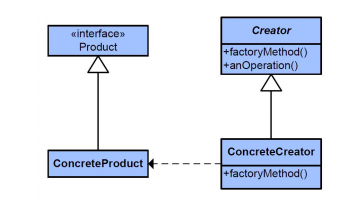
\includegraphics[width=100mm,height=60mm]{Slike/dp_factory_method.png}
    \end{center}
  \end{figure} 

\section{Objasniti kada se i kako primenjuje uzorak Strategija.}
  Definisati familiju algoritama, enkapsuliraj svaki. Ovaj obrazac reprezentuje skup različitih
  strategija, gde se primenjuje jedna, odgovarajuća strategija u zavisnosti od konteksta. \\
  \textbf{Koristi se kada:}
  \begin{itemize} 
    \item se mnoge srodne klase razlikuju samo u njihovom ponašanju. 
          Strategija obezbeđuje način da podesite klasu sa jednim od mnogih ponašanja.
    \item potrebne su različite varijante nekog algoritma. 
          Strategija može da se koristi kada se ove varijante sprovode kao hijerarhije klasa algoritama.
    \item algoritam koristi podatke o kojima klijenti ne treba da znaju. 
          Obrazac Strategija se ovde upotrebljuje da bi se izbeglo izlaganje složenih 
          struktura podataka specičnih za algoritam.
    \item klasa definiše mnoga ponašanja, koja se pojavljuju kao višestruke 
          uslovne naredbe u njenim operacijama. Umesto mnogih uslovnosti, 
          pomeriti srodne uslovne grane u zasebnu klasu Strategije.
  \end{itemize}

\section{Skicirati dijagram klasa uzoraka za projektovanje Strategija.}
  \begin{figure}[H]
    \begin{center}
        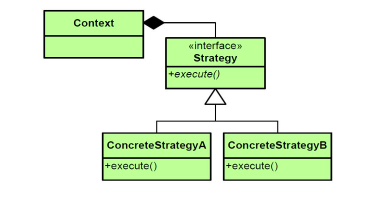
\includegraphics[width=100mm,height=60mm]{Slike/dp_strategy.png}
    \end{center}
  \end{figure} 

\section{Objasniti kada se i kako primenjuje uzorak Dekorater.}
  Dekorater omogućava da se funkcionalnosti objekta povećaju bez menjanja njene strukture. Pravi se
  dekorater klase koji predstavlja okvir za originalnu klasu, koji proširuje njenu funkcionalnost,
  ne menjajući njenu suštinu. \\
  \textbf{Koristi se kada:}
  \begin{itemize}
    \item je potrebno da se dodaju odgovornosti pojedinačnim objektima, 
          a da to ne utiče na druge objekta.
    \item je potrebno dodati neke obaveze koje se mogu povući.
    \item Kada je proširivanje potklase nepraktično. Ponekad je moguć veliki broj nezavisnih
          ekstenzija, što bi proizvelo eksploziju uz svaku kombinaciju.
  \end{itemize}
  
\section{Skicirati dijagram klasa uzoraka za projektovanje Dekorater.}
  \begin{figure}[H]
    \begin{center}
        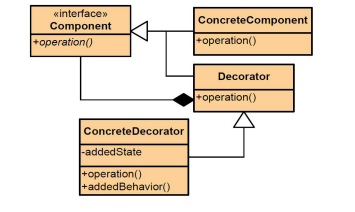
\includegraphics[width=100mm,height=60mm]{Slike/dp_decorator.png}
    \end{center}
  \end{figure} 

\section{Objasniti kada se i kako primenjuje uzorak Složeni objekat (Sastav, Composite).}
  Ponekad je potrebno da grupu objekata tretiramo isto kao i jedan objekat. Tada koristimo sastav
  kao uzorak za projektovanje. \\
  \textbf{Koristi se kada:}
  \begin{itemize}
    \item je potrebno predstaviti celu hijearhiju objekata;
    \item je potrebno ignorisati razliku između kompozije objekata i jednog objekta.
  \end{itemize}

  Primer: Na kursu KK (Konstrukcija Kompilatora) se implementira kompilator 
  za deo jezika $Paskal$ koji generiše apstraktno sintaksno stablo na osnovu koda. Tu naredba(čvor) 
  može da bude tipa naredba ispiši ili naredba dodele, a može da bude blok koji 
  se sastoji od niza naredbi. U ovom slučaju je poželjno koristiti sastav. 

\section{Skicirati dijagram klasa uzoraka za projektovanje Slozeni objekat (Sastav, Composite).}
  \begin{figure}[H]
    \begin{center}
        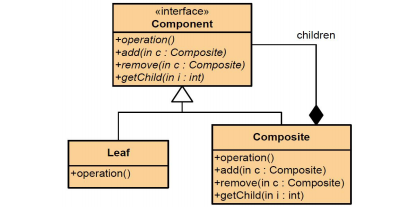
\includegraphics[width=100mm,height=60mm]{Slike/dp_composite.png}
    \end{center}
  \end{figure}   

\section{Objasniti kada se i kako primenjuje uzorak Unikat (Singleton).}
  Koristi se kad je potrebno osigurati da klasa ima samo jednu instancu i obezbediti globalnu 
  tačku pristupa za nju.

\begin{lstlisting}
  #include <iostream>

  class Singleton {
  private:
      static Singleton* instance;
  
      Singleton() { count++; }
      Singleton(const Singleton& s) = delete;
      Singleton& operator=(const Singleton& s) = delete;
  
  public:
      static Singleton* create()
      {
          if(!instance)
              instance = new Singleton;
          return instance;
      }
      static int count;
  };
  Singleton *Singleton::instance = 0;
  int Singleton::count = 0;
  
  int main()
  {
      Singleton* singleton = singleton->create();
      std::cout << singleton->count << std::endl;
      Singleton* doubleton = doubleton->create();
      std::cout << doubleton->count << std::endl;
  
      return 0;
  }\end{lstlisting}

\section{Skicirati dijagram klasa uzoraka za projektovanje Unikat (Singleton).}
  \begin{figure}[H]
    \begin{center}
        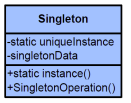
\includegraphics[width=40mm,height=30mm]{Slike/dp_singleton.png}
    \end{center}
  \end{figure}  

\section{Objasniti kada se i kako primenjuje uzorak Posetilac (Visitor).}
  Poenta uzorka posetilac je mogućnost da se definiše nova operacije bez vršenja promena na
  već postojećoj strukturi objekta. Posetilac ne zna nužno kojeg je tipa objekat (ako se 
  pristupa objektu preko pokazivača ili reference), ali objekat sigurno zna kojeg je on tipa. Zbog toga je potrebno
  da objekat prihvati posetu od posetioca kako bi posetilac mogao da izvrši odgovarajuću operaciju.\\
  \textbf{Koristi se kada:}
  \begin{itemize}
    \item struktura objekta sadrži mnoge klase objekata sa različitim interfejsima i potrebno 
          je izvršiti operacije nad ovim objektima koji zavise od njihovih konkretnih klasa;
    \item je potrebno izvršiti mnoge razne nepovezane operacije zajedno;
    \item kada je struktura objekata deljena od strane dosta aplikacija, u posetilac se mogu
          staviti operacije samo onih aplikacija kojima je to potrebno;
    \item kada se klase koje određuju strukturu objekata retko menjaju, ali je često potrebno
          definisati novu operaciju nad tom strukturom.
  \end{itemize}

\section{Skicirati dijagram klasa uzoraka za projektovanje Posetilac (Visitor).}
  \begin{figure}[H]
    \begin{center}
        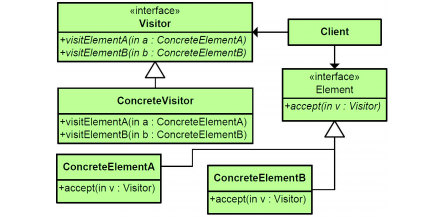
\includegraphics[width=100mm,height=50mm]{Slike/dp_visitor.png}
    \end{center}
  \end{figure} 

\section{Objasniti kada se i kako primenjuje uzorak Posmatrač (Observer).}
  Posmatrač se koristi kada postoji jedan-ka-više veza između objekata tako da ako se desi promena 
  na određenom objektu potrebno je automatski obavestiti sve druge objekte koje zavise od njega.\\
  \textbf{Koristi se kada:}
  \begin{itemize}
    \item apstrakcija ima dva aspekta, gde je jedan zavisan od drugog. Enkapsulacija ovih aspekata
          u odvojenim objektima omogućava da ih menjamo i koristimo samostalno;
    \item kada promena u jednom objektu zahteva promenu u drugim objektima, gde je broj
          objekata koji treba da se promene nepoznat;
    \item kada objekat treba da obavesti druge objekte bez pretpostavke o tome kojeg su tipa ti objekti.
  \end{itemize}

\section{Skicirati dijagram klasa uzoraka za projektovanje Posmatrač (Observer).}
  \begin{figure}[H]
    \begin{center}
        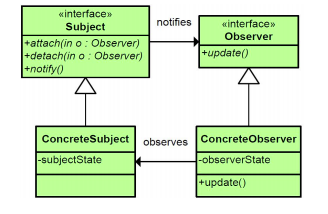
\includegraphics[width=100mm,height=45mm]{Slike/dp_observer.png}
    \end{center}
  \end{figure} 

\section{Objasniti kada se i kako primenjuje uzorak Apstraktna fabrika (Abstract Factory).}
  Apstraktna fabrika se koristi kada je potrebno kreiranje porodice srodnih ili zavisnih objekata
  bez navođenja njihove konkretne klase. \\
  \textbf{Koristi se kada:}
  \begin{itemize}
    \item sistem treba da bude nezavisan od toga kako su njegovi proizvodi kreirani, 
          od sastava, i načina predstavljanja.
    \item sistem treba da bude konstruisan sa više od jedne porodica klasa.
    \item familija srodnih klasa je dizajnirana da se koriste zajedno, 
          i treba da sprovede ovo ograničenje.
    \item je potrebno da se obezbedi biblioteka klase proizvoda, 
          a takođe je potrebno da se otkrije samo njihov interfejs, 
          a ne i njihova implementacija.
  \end{itemize}

  Primer: Implementacija više tema (\textit{light/dark}) za interfejs. \cite{medium_abstractfactory}

\section{Skicirati dijagram klasa uzoraka za projektovanje Apstraktna fabrika (Abstract Factory).}
  \begin{figure}[H]
    \begin{center}
        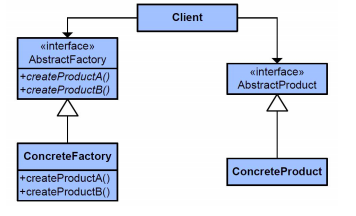
\includegraphics[width=100mm,height=45mm]{Slike/dp_abstract_factory.png}
    \end{center}
  \end{figure} 

\section{Šta je Agilni razvoj softvera?}
  Agilni razvoj softvera (ARS) je familija metodologija nastala krajem 80-tih, početkom 90-tih.
  Naziv je oblikovan 2001. godine kada je formulisan \textbf{Manifest agilnog razvoja softvera}. 
  Agilni  razvoj softvera ima dosta sličnosti sa objektno orijentisanim metodologijama, ali sa
  drugačijem pristupu planiranja. Uglavnom se pretpostavlja upotreba tehnika OO projektovanja i
  programiranja. Propisuje skup principa tehnika za njihovo ostvarivanje. Promoviše dinamičan 
  i disciplinovan timski rad. Brzo se reaguje na svaku promenu u okruženju.
  \cite{agilemanifesto}\cite{ss_agile_manifesto}\\
  Agilni razvoj \textbf{NIJE}:
  \begin{itemize}
    \item Odsustvo sistematičnosti i strukturnog prisustva;
    \item Anarhično ili svojevoljno ponašanje članova tima;
    \item Potpuno odsustvo dokumentacije (softver bez dokumentacije ne vredi ništa);
    \item Selektivna primena samo nekih od principa ARS-a;
    \item Najlakši metod razvoja softvera;
    \item Univerzalno rešenje za sve probleme;
    \item Pravi način rada za neiskusne ili nedovoljno stručne programere ili timove.
  \end{itemize}

\section{Navesti osnovne pretpostavke Manifesta agilnog razvoja.}
  Manifest prepoznaje osnovne 4 pretpostavke na kojima počiva agilni razvoj i određuje 12 osnovnih
  principa agilnih metodologija. Konkretne agilne metodologije mogu imati dodatne pretpostavke, 
  principe i da određuju metode i tehnike kojima se principi ostvaruju. \\
  \textbf{Pretpostavke:}
  \begin{itemize}
    \item Pojedinci i saradnja ispred procesa i alata;
    \item Funkcionalan softver ispred iscrpne dokumentacije;
    \item Saradnja sa klijentom ispred pregovaranja;
    \item Reagovanje na promene ispred praćenja plana.
  \end{itemize}

\section{Objasniti pretpostavku agilnog razvoja da su pojedinci i saradnja ispred procesa i alata.}
  Ima smisla staviti pojedince i saradnju ispred procesa i alata, jer su ljudi ti koji odgovaraju
  na zahteve posla i razvijaju procese. Ako procesi ili alati vode razvoj, onda su manje šanse 
  da tim uspešno odgovori na promene ili ispoštuje zahteve klijenta. Komunikacija
  je primer gde može da se predstavi razlika između vrednovanja pojedinaca naspram vrednovanja
  procesa. U slučaju vrednovanja pojedinaca, komunikacija dolazi prirodno kada je potrebna, a u 
  slučaju vrednovanja procesa je komunikacija zakazana i zahteva konkretnu temu. \\
  \indent Ljudi predstavljaju najvažniji deo uspešnog razvoja. Dobar proces ne može uspeti sa lošim ljudima,
  dok loš proces i najbolje ljude čini neproduktivnim. Veoma je bitno da se izgradi dobar tim u kojem
  će biti dobra saradnja. Dobri alati su dobrodošli, ali previše pažnje posvećeno alatima je 
  jednako loše kao potpuno odsustvo alata.

\section{Objasniti pretpostavku agilnog razvoja da je funkcionalan softver ispred iscrpne dokumentacije.}
  Agilne metodologije ne eliminišu dokumentaciju, jer je softver bez dokumentacije beskoristan.
  Međutim, agilne metodologije više vrednuju funkcionalan softver nego dokumentaciju. Taj stav ima 
  smisla, jer je osnovni cilj softver, a ne dokumentacija. Korisno je pisati popratnu dokumentaciju, 
  ali bez preteranog iscrpljivanja. 

\section{Objasniti pretpostavku agilnog razvoja da je saradnja sa klijentom ispred pregovaranja.}
  Softver ne može da se naručuje kao nameštaj, jer u svakom malo složenijem slučaju je praktično 
  nemoguće da se napiše opis zadatka i prepusti nekome da se napravi softver. Bitna je aktivna
  komunikacija sa klijentom i tokom razvoja. Klijent nije tehničko lice i ne može da zna precizno
  šta želi, a ne može ni da zna šta razvojni tim može da uradi za njega. Zbog toga uspeh projekta 
  zavisi od redovne komunikacije sa klijentom.

\section{Objasniti pretpostavku agilnog razvoja da je reagovanje na promene ispred praćenje plana.}
  Tradicionalno je promena smatrana kao dodatan trošak, zbog čega je izbegavana. Promene su 
  neizbežne i sigurno nastupaju, a pitanje je samo kada će nastupiti i koje će promene nastupiti.
  Zbog toga je bitno da razvojni tim bude sposoban da reaguje na promene. Takođe je potrebno da plan
  bude fleksibilan kako bi se lako prilagodio tim promenama. Planiranje treba da se vrši na kraći
  period, jer se detaljni planovi, iako su koristni, teško održavaju na dužem periodu. Naravno,
  vizija i glavni ciljevi su neophodni i bitno je da se zna šta se pravi (ipak, 
  ponekad se i oni menjaju).

\section{Navesti bar 8 principa agilnog razvoja softvera.}
  \begin{enumerate}
    \item Najviši prioritet je zadovoljiti klijenta kroz rano i neprekidno isporučivanje vrednog 
          softvera.
    \item Treba uvek otvoreno prihvatani promene, čak i u kasnim fazama razvoja. Promene se uvažavaju 
          kao sredstvo postizanja kvaliteta za klijenta.
    \item Softver treba isporučivati često, od nekoliko nedelja do nekoliko meseca sa preferencom 
          na što kraćem periodu.
    \item Poslovni ljudi i razvijaoci moraju sarađivati svakodnevno na projektu.
    \item Zasnivati projekat na motivisanim pojedincima. Pružati im okruženje i potrebnu podršku
          i imati poverenja da će obaviti posao.
    \item Najefikasniji način za razmenu informacija u okviru razvojnog tima je razgovor
          lice u lice. Timovi bi trebalo da rade u istoj zgradi.
    \item Funkcionalan softver je osnovno merilo napretka.
    \item Agilni procesi promovišu uzdržani razvoj. Sponzori, razvijaoci i korisnici bi trebalo
          da održavaju ujednačeni ritam. 
    \item Neprekidno posvećivanje pažnje tehničkoj doteranosti i dobrom dizajnu podiže agilnost.  
    \item Jednostavnost, umetnost da se maksimizuje količina posla koji se ne obavlja, je od
          suštinskog značaja.
    \item Najbolje arhitekture, zahtevi i projekti potiču iz samoorganizovanih timova. 
    \item U redovnim intervalima tim mora da sagleda svoj rad i mogućnosti unapređivanja svoj ponašanja
          i efikasnosti. \cite{ss_agile_manifesto}
  \end{enumerate}

\section{Navesti bar 3 metodologije agilnog razvoja softvera.}
  \begin{enumerate}
    \item Agilno modeliranje
    \item Agilan objedinjen proces (AUP)
    \item Ekstremno programiranje (XP)
    \item Otvoren objedinjen proces (OpenUP)
    \item Scrum
  \end{enumerate}

\section{Šta je ekstremno programiranje?}
  Jedna od najpoznatijih agilnih metodologija. Čini da jednostavne, međusobno zavisne metode u skladu
  sa pretpostavkama i principima ARS i preciznije opisuje ostvarivanja principa ARS. Trenutno nije
  među najzastupljenijim metodologijama, ali se principi ove metode koriste.\\

  Zašto se zove \textbf{,,Extreme Programming``}? \\
    \indent - Zato što tako zvuči ,,kul``. \\
    \indent - Ovaj naziv su odredili menadžeri, ne programeri.\\
    \indent - Prikladnija alternativa: \textbf{,,BusinessValueOrientedProgramming``}. \cite{wikic2_xp}

\section{Navesti bar 8 metoda ekstremnog programiranja.}
  \begin{enumerate}
    \item Klijent je član tima (The Customer)
    \item Korisničke celine (Stories)
    \item Kratki ciklusi (Lifecycle, Weekly Cycle, Quarterly Cycle)
    \item Praćenje toka razvoja
    \item Testovi prihvatljivosti (Acceptance Tests)
    \item Programiranje u paru (Pair Programming)
    \item Razvoj vođen testovima (Test-Driven Development)
    \item Kolektivno vlasništvo (Collective Code Ownership)
    \item Neprekidna integracija (Continuous Integration)
    \item Uzdržan ritam (Sustainable pace)
    \item Otvoren radni prostor (Open Work Space)
    \item Igra planiranja (Planning Game)
    \item Jednostavan dizajn (Simple Design)
    \item Refaktorisanje (Refactoring)
    \item Metafora (Metaphore)\cite{aa_xp}\cite{ab_xp}
  \end{enumerate}

\section{Objasniti metod ekstremnog programiranja ,,Klijent je član tima``.}
  Metoda ,,Klijent je član tima`` (eng. ,,The customer``) podrazumeva da u timu,
  pored programera, mora da postoji i barem jedan predstavnik klijenata. Idealno je
  da je predstavnik stalno tu i sarađuje sa razvijaocima. U ekstremnom programiranju
  klijent ima uloga člana tima. 

\section{Objasniti metod ekstremnog programiranja ,,Korisničke celine``.}
  Metoda ,,Korisničke celine`` (eng. ,,Stories``) podrazumeva da postoje kratka objašnjenja
  šta klijent želi u okviru neke celine koju razvojni tim treba da implementira. Radi okvirnog
  planiranja potrebno je sagledati zahteve, ali ne i potpuno precizne elemente zahteva. Neophodno
  je znati gde i kakvih detalja ima, ali ne i same detalje (detalji se menjaju tokom vremena). 
  Prve (grube) procene rokova i troškova služe samo za upravljanje prioriteta. Primer:
  \begin{figure}[H]
    \begin{center}
        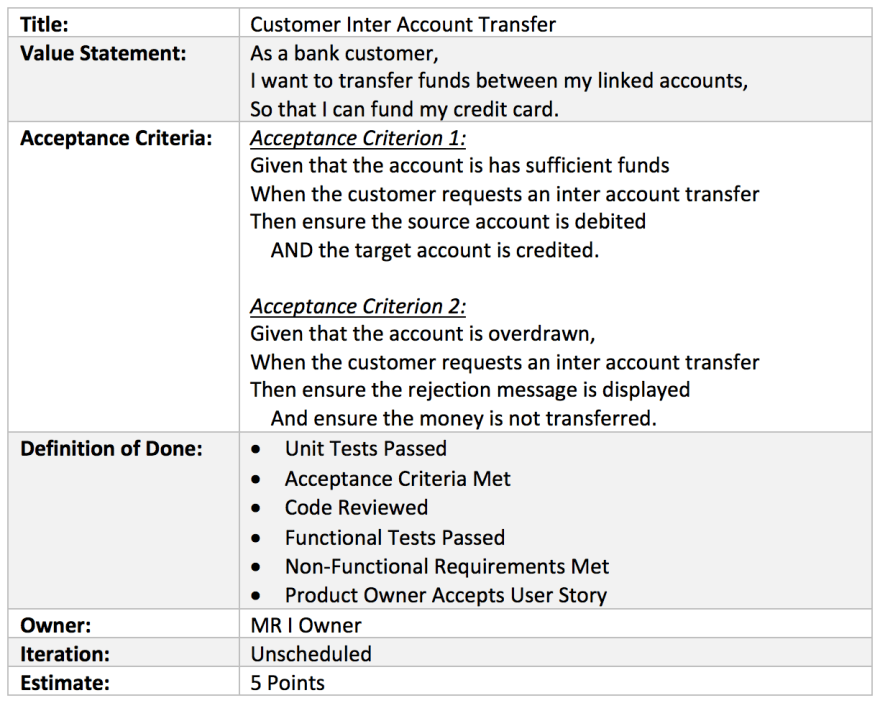
\includegraphics[width=100mm,height=80mm]{Slike/korisnicka_prica.png}
    \end{center}
  \end{figure} 

  Korisničke celine služe kao referenca na nešto što će se detaljnije razmatrati kada dođe red
  na implementaciju. 

\section{Objasniti metod ekstremnog programiranja ,,Kratki ciklusi``.}
  Metoda ,,Kratki ciklusi`` (eng. ,,Lifecycle``) podrazumevaju redovne iteracije (eng. Weekly Cycle) i 
  izdanja (eng. Quarterly Cycle, release).\\
  
  \textbf{Iteracija:} Sinonim nedeljni ciklus već dosta govori o samom pojmu iteracija.
  Iteracije su manji ciklusi koji traju relativno kratko, jednu-dve nedelje. 
  Iteracija počinje sa određivanjem budžeta i dužine trajanja na osnovu odabranih
  korisničkih celina (bira ih klijent uz konsultaciju sa razvojnim timom) koji bi trebalo 
  da budu urađeni u okviru te iteracije. Zadatak je da razvojni tim na kraju iteracije
  da klijentu deo softvera (rađen po prethodnom dogovoru) koji klijent može da testira.

  \textbf{Izdanje:} Takođe sinonim, tromesečni ciklus dosta govori i samom pojmu izdanja.
  Izdanje obuhvata nekoliko iteracija (primer: 6). Ovo se odnosi na neku značajniju celinu
  u odnosu na delove koji se obrađuju u okviru iteracija. Bitno je da klijent ostavi generalni
  plan koji predstavlja ,,Pogled na šumu`` programerima dok su oni na ,,drveću``. Sastoji 
  se od korisničkih celina sa procenama i prioritetima. Uokvirno se definišu sadržaji pojedinačnih 
  iteracija. Iteracija mogu da se menjaju, a čak može i da se promeni broj iteracija u okviru 
  izdanja (nisu poželjne veće promene). 
  
\section{Objasniti metod ekstremnog programiranja ,,Testovi prihvatljivosti``.}
  Metoda ,,Testovi prihvatljivosti`` (eng. ,,Acceptance Tests``) podrazumeva 
  da postoje testovi u okviru korisničkih celina. Ove testove određuje klijent i pišu se 
  neposredno ili čak paralelno sa implementacijom iste celine. Testovi se po mogućnosti automatizuju. 
  Ovi testovi se ponavljaju svaki put po izgradnji sistem (nekoliko puta dnevno).
  \cite{xporg_acceptance_tests}\\
  Primer alata: \textit{Selenium}. 

\section{Objasniti metod ekstremnog programiranja ,,Programiranje u paru``.}
  Metoda ,,Programiranje u paru`` (eng. ,,Pair programming``) podrazumeva da se delovi
  softvera realizuju u paru (programera), gde dvoje ljudi sede jedan pored drugog za istom
  mašinom (,,Dve glave su pametnije od jedne``). Jedan član tima piše kod, a drugi komentariše
  i ispravlja kolegu ako je potrebno. \\
  \indent Uloge se menjaju više puta. Istraživanja pokazuju da
  se ovako značajno smanjuje broj grešaka, a greška koštaju, pa samim tim se smanjuje
  cena projekta. Ovo podrazumeva da pojedinci mogu da sarađuju. Bitno je naglasiti
  da specijalnost i dalje ostaje na pojedincima, ali su drugi ipak upoznati sa rezultatima.\\
  \indent U okviru iteracije svaki član tima mora da radi sa svim članovima tima i da radi skoro na
  svim delovima iteracije. Ovim se informacije veoma efikasno razmenjuju i svaki član tima je
  upoznat sa svakim delom projekta.\\

\section{Objasniti metod ekstremnog programiranja ,,Razvoj vođen testovima``.}
  Metoda ,,Razvoj vođen testovima`` (eng. ,,Test-Driven Development) podrazumeva da razvijanje
  počinje pisanjem testova. Naravno, ti testovi na početku ne mogu da prođu, jer funkcionalnosti
  nisu implementirane. Nakon napisanih testova se piše kod koji prolazi date testove. 
  Programer naizmenično piše testove i kod koji prolazi te testove. \\
  \textbf{Prednosti koje ova metoda donosi su:}
  \begin{itemize}
    \item Uz kod se dobija kompletna kolekcija testova;
    \item Testovi mogu da se koriste da se proveri da li jedinica koda radi ispravno ili ne;
    \item Sprečava nastajanje grešaka prilikom naknadnih izmena;
    \item Pomaže prilikom refaktorisanja;
    \item Metod vrši pritisak da se razdvajaju jedinice koda, čime se dobija kvalitetniji dizajn.
  \end{itemize}

\section{Objasniti metod ekstremnog programiranja ,,Kolektivno vlašnistvo``.}
  Metoda ,,Kolektivno vlašnistvo`` (eng. ,,Collective code ownership``) podrazumeva
  da svako može da proveri bilo koji deo modula i da ga uporedi. Nijedan programer nije
  pojedinačno odgovoran za bilo koji konkretan modul ili tehnologiju. Svako može da 
  radi na bilo kojoj oblasti. To ne znači da se specijalnosti i dalje ne poštuju. Svako će
  najviše da radi u svojoj struci, ali može da se priključi i u druge celine i da uči od
  drugih specijalista.

\section{Objasniti metod ekstremnog programiranja ,,Neprekidna integracija``.}
  Metoda ,,Neprekidna integracija`` (end. ,,Continuous process``) podrazumeva da se intenzivno 
  koristi sistem za upravljenje verzijama, gde se na dnevnom nivou više puta postavlja nova
  verzija koda. Najveća prednost ove metode je to što se problemi prilikom integracije vrlo 
  brzo prepoznaju i rešavaju. \\
  \indent Obično se prave testovi i produkcioni kod koji se kasnije, u nekom pogodnom trenutku (relativno 
  često), integrišu. Pre svake integracije se proverava da li svi testovi prolaze. \\
  \textbf{Prednosti:}
  \begin{itemize}
    \item Postupak debagovanje je značajno lakši;
    \item Testovi ukazuju da postoji problem (ukazuju na njegovu prostornu i vremensku lokaciju);
    \item Istorija verzija omogućava sužavanje prostorne i vremenske lokacije nastajanja problema.
  \end{itemize}

\section{Objasniti metod ekstremnog programiranja ,,Uzdržan ritam``.}
  Metoda ,,Uzdržan ritam`` (eng. ,,Sustainable pace``) podrazumeva zabranu prekovremenog rada.
  Jedini izuzetak za prekovremeni rad je poslednja nedelja izdanja: ,,Ako je tim dovoljno blizu
  cilja, \textit{sprint} je dopušten. \\

  ,,Razvoj softvera nije \textit{sprint}, nego maraton.``  (R. Martin)\\

  \textbf{Prednosti:} Bolji odnosu u timu, manja rasterećenost članova tima, manji broj grešaka i
  efikasnija iskorisćenost radnog vremena.

\section{Objasniti metod ekstremnog programiranja ,,Otvoren radni prostor``.}
  Metoda ,,Otvoreni radni prosto`` (eng. Open work space) podrazumeva da tim radi u jednoj
  velikoj otvorenoj prostoriji, gde se na svakom stalo nalaze dve ili tri radne stanice, 
  par stolica, a na zidovima su table i panoi. Uobičajni ton je tiha komunikacija i svi mogu
  međusobno da komuniciraju. Iako u teoriji ova metoda zvuči loše, u praksi se pokazuje da znatno 
  poboljšava efikasnost.

\section{Objasniti metod ekstremnog programiranja ,,Igra planiranja``.}
  Metoda ,,Igra planiranja`` (eng. Planning Game) podrazumeva podelu odgovornosti između klijenta
  i razvojnog tima, gde klijent odlučuje šta je značajna karakteristika softvera, a razvijaoci
  odlučuju koliko bi ta karakteristika koštala. \\
  \textbf{U okviru planiranja izdanja postoje tri faze:}
  \begin{itemize}
    \item \underline{Faza istraživanja:} Klijenti definišu zahteve preko korisničkih priča;
    \item \underline{Faza ivršavanja:} Planiranje i implementacija klijentskih zahteva;
    \item \underline{Faza upravljanja:} Prethodno definisani planovi se usaglašavaju sa zahtevima projekta.
  \end{itemize}
  \textbf{U okviru planiranja iteracije postoje tri faze:}
  \begin{itemize}
    \item \underline{Faza istraživanja:} Beleže se zahtevi projekta;
    \item \underline{Faza ivršavanja:} Podela poslova po razvijaocima i njihova izrada;
    \item \underline{Faza upravljanja:} dobijeni rezultati se detaljnije upoređuju sa početnim zahtevima.
  \end{itemize}

\section{Objasniti metod ekstremnog programiranja ,,Jednostavan dizajn``.}
  Metoda ,,Jednostavan dizajn`` (eng. Simple design) podrazumeva da se pravi ono što je u tom
  trenutnu potrebno, bez komplikovanja unapred. Cilj je da dizajn bude što jednostavniji i što
  izražajniji. Pažnja se posvećuje samo onome što je planirano za tekuću iteraciju i ne razmatra
  se ono što će možda doći kasnije. Razvoj obično ne potiče od infrastrukture. \\
  \textbf{Tri osnovna pravila:}
  \begin{itemize}
    \item \textbf{Razmotriti prvo najjednostavnije rešenje koje bi moglo da uradi posao:}
          Cilj je da se sa što manje rada i u što kraćem vremenu doći do cilja, a dizajn se
          može unapređivati kasnije. Primeri:
          \begin{itemize}
            \item Ako nešto može da se reši preko datoteka, nema potrebe da se odmah upliću
                  baze podataka ili objekti srednjeg sloja.
            \item Ako nešto može bez paralelnog izračunavanja, valja tako i rešiti.
          \end{itemize}
    \item \textbf{,,Neće biti potrebno! ``:} Kad god se postavlja pitanje da li je nešto potrebno 
          ili ne onda je odgovor: ,,Neće biti potrebno! ``. Izbegava se dodavanje nečega što će možda 
          biti potrebno. Cilj je izbegavati komplikovan dizajn radi nečega što neće biti potrebno.
    \item \textbf{,,Jedanput i samo jedanput``:} Ekstremno programiranje ne dopušta ponavljanje u kodu.
          Kada god se naiđe na ponavljanje u kodu, ono se mora ukloniti. Čak i kad su delovi koda
          veoma slični, oni se moraju apstrahovati. Cilj je minimizovati redundantnost koda
          apstrahovanjem.
  \end{itemize}
  \textbf{Napomena:}
  \begin{itemize}
    \item Razmatranje najjednostavnijeg rešenja nikako ne znači da kod sme da bude loše dizajniran.
    \item ,,Jednostavno`` ne znači ,,na brzinu`` ili ,,nepažljivo``.
  \end{itemize}

\section{Objasniti metod ekstremnog programiranja ,,Refaktorisanje``.}
  Metoda ,,Refaktorisanje`` (eng. ,,Refactoring``) podrazumeva učestalo popravljanje i održavanje
  kvaliteta koda refaktorisanjem. 
  \begin{itemize}
    \item \textbf{Šta je refaktorisanje?} Refaktorisanje je proces koji se sastoji iz niza
          manjih transformacija nad kodom bez menjanja ponašanja koda. Ove transformacije
          služe samo za poboljšanje kvaliteta koda. Refaktorisanjem se ne dodaje nova funkcionalnost.
    \item \textbf{Zašto refaktorisati?} ,,Kod je kvarljiv`` R. Martin\\
          Jednom napisan kod nije gotov, jer će u jednom trenutku biti potrebno da se izvrši
          neka promena. Postepenim menjanjem dizajna koda se kod kvari. Ako dodajemo
          neku novu funkcionalnost na kod, njegov kvalitet može da opadne. Ekstremno
          programiranje se suprostavlja lošem kvalitetu koda čestim refaktorisanjem.
          Testovi su jako korisni prilikom refaktorisanja, jer oni proveravaju da li se
          ponašanje koda promenilo.
    \item \textbf{Kada refaktorisati?} Refaktorisanje treba stalno da se primenjuje u hodu,
          kada se primeti da neka izmena narušava postojeći dizajn. Refaktorisanje se 
          vrši paralelno sa razvojem testova i produkcionog koda. Dobra je praksa da se 
          kod refaktoriše svaki put pre nego što se doda nova funkcionalnost. 
  \end{itemize}

\section{Objasniti metod ekstremnog programiranja ,,Metafora``.}
  Metoda ,,Metafora`` (eng. ,,Metaphore``) podrazumeva da postoji velika slika čitavog sistema
  koja predstavlja viziju sistema kao celine. Iz metafore (ne)posredno potiču svi konkretni moduli
  i zahtevi. \\
  \begin{itemize}
    \item Ako ne znamo šta želimo sa projektom, onda ne treba ni da ga razvijamo. \\
    \item Često se realizuje u vidu rečnika pojmova koji identifikuju najvažnije koncepte sistema 
          i problema koji bi on trebalo da reši.
  \end{itemize}

\section{Šta je ,,Razvoj vođen testovima``?}
  Razvoj vođen testovima je stil vođenja razvoja koji kaže sledeću stvar: Ako treba nešto 
  da se isprogramira, pre nego što se isprogramira, prvo se piše deo koda koji proverava
  da li taj kod radi kako treba. Prvo se pišu testovi, potom se piše kostur datog koda koji
  u početku ne radi (ne prolazi testove), ali omogućava da se kod prevede. Nakon toga se piše kod.\\

  Kada se priča o razvoju vođen testovima, onda se prvenstveno priča o testovima jedinica (eng. unit
  test).\\

  \noindent \textbf{Napomena:} Pisanje testova nije dokaz korektnosti koda!

\section{Navesti i objasniti vrste testova softvera.}
  \begin{itemize}
    \item \textbf{Testovi jedinica (Unit tests):} Testovi jedinica koda. Jedinica koda
          može biti funkcija, metod, klasa, komponenta, \dots
    \item \textbf{Integracioni testovi (Integration tests):} Testovi kojim se proverava da li
          moduli funkcionišu zajedno.
    \item \textbf{Sistemski testovi (System Tests):} Testiranje sistema kao celine.
    \item \textbf{Testovi prihvatljivosti (Acceptance Tests):} Testiranje iz ugla korisnika. Često
          se izvode preko skriptova koji simuliraju ili emuliraju korisnički interfejs.
  \end{itemize}

\section{Navesti i objasniti ukratko osnovne principe razvoja vođenog testovima.}
  Razvoj vođen testovima je princip koji kombinuje princip ,,Testovi prethode kodu`` i 
  sistematičnost (ne sme da postoji nijedan deo koda koji nije pokriven prilikom pravljenja
  testova). Ovaj princip takođe podrazumeva refaktorisanje koda nakon što prođu svi testovi.

\section{Objasniti princip razvoja vođenog testovima ,,Testovi prethode kodu`` i način njegove primene.}
  \noindent \textbf{Osnovna pravila:}
  \begin{itemize}
    \item Pre pisanja koda se prave odgovarajući testovi.
    \item Nijedna funkcija programa se ne razvija sve dok ne postoji test koji ne uspeva zbog 
          njenog odsustva.
    \item Nijedna linija koda ne sme da se dodaje dok postoji test koji zbog nje ne uspeva.
    \item Tek nakon definisanih testova mogu da se implementiraju funkcionalnosti koje
          zadovoljavaju uslove tih testova.
  \end{itemize}
  Svaka iteracija počinje sa pisanjem testova. Ti testovi se često najpre ne prevode zbog nedostataka
  odgovarajućih metoda ili klasa. Zatim se piše kostur koji omogućava da se kod prevede (obično
  se vraćaju netačni rezultati, npr. funkcija vraća nulu). Nakon toga se piše kod koji zadovoljava
  testove. \\

  \noindent \textbf{Princip ,,Mali Koraci``}:
  \begin{itemize}
    \item Treba testirati što manje celine;
    \item Ako prolaze testovi, a postoji bag, onda testovi nisu dovoljno dobri;
    \item Iteracije pisanja testova i pisanje koda se brzo smenjuju;
    \item Poželjno je da testovi i kod evoluiraju zajedno gde testovi malo prethode kodu;
    \item Nije dobro napisati veliki broj testove bez odgovarajućeg koda;
  \end{itemize}

\section{Objasniti princip razvoja vođenog testovima ,,Sistematičnost``.}
  Princip sistematičnosti podrazumeva da svaka karakteristika softvera mora da bude pokrivena
  testovima. Bitno je da svi opšti slučajevi budu pokriveni, a i neki specijalni slučajevi.
  Svi granični slučajevi moraju da budu obuhvaćeni testovima. Svaka linija koda mora biti
  testirana. \\

  \noindent \textbf{Tehnike:}
  \begin{itemize}
    \item \textbf{Softver se razvija od vrha prema dnu:} Potrebno je imati ,,stub`` (privremeni deo 
          koda) u kodu koji implementiraju interfejs i slične metode tako da ne rade ništa. Njihova
          svrha je samo da kod može da se prevede. 
    \item \textbf{Softver se razvija od dna prema vrhu:} Testira se pomoću izvođača (drajvera) koji
          predstavljaju privremeni deo koda koji koriste manje funkcionalne celine u odsustvu
          velikih funkcionalnih celina koje tek treba da se implementiraju.
  \end{itemize}

\section{Navesti osnovne uloge testova.}
  \begin{enumerate}
    \item Predstavljaju vid verifikacije;
    \item Pomažu pri refaktorisanju;
    \item Predstavljaju vid dokumentacije;
    \item Omogućavaju više uglova posmatranja koda;
    \item Pomažu pri debagovanju;
  \end{enumerate}

\section{Objasniti ulogu testova kao vida verifikacije softvera.}
  Kolekcija testova omogućava progameru da proverava da li jedinica koda radi ispravno ili ne.
  Za svaku funkciju programa postoje odgovarajući testovi koji proveravaju njenu ispravnost. 
  Testovi omogućavaju da se proveri da li je nešto možda loše izmenjeno. Takođe, pomažu da se rano
  prepoznaju greške na nivou koda ili na konceptualnom nivou. Testovi vrše dodatni pritisak
  na razdvajanje jedinica koda, što dovodi do boljeg dizajna. 

\section{Objasniti ulogu testova u okviru refaktorisanja.}
  Refaktorisanje podrazumeva izmene na kodu u cilju poboljšanja kvaliteta koda, ali
  prilikom refaktorisanja ne sme doći do promene ponašanja koda. Testovi mogu da provere
  da li je došlo do promene ponašanja koda prilikom refaktorisanja. Ako izmene narušavaju
  pravila, onda ne bi trebalo da prođu testove.

\section{Objasniti ulogu testova u kontekstu ugla posmatranja koda.}
  Pravljenje testova postavlja programera u poziciju korisnika. U prvom planu su interfejs 
  jedinice koda i apstrakcija njenog ponašanja. Testovima se omogućava lako upotrebljiv kod.
  Takođe se dobije lako proverljiv kod, što se kasnije može teško postići ako sistem nije 
  dobro oblikovan.
  
\section{Objasniti ulogu testova kao vida dokumentacije.}
  Testovi predstavljaju oblik specifikacije zahteva (prikazuju jednostavnije zahteve koje 
  program u radu treba da ispuni). Opisuju uslove funkcionisanja koda i način njegove upotrebe 
  (primer upotrebe interfejsa). Testovi predstavljaju karakteristične primere (granični slučajevi). 
  Prednost testova kao dokumentacije je to što je takav tip dokumentacije konstantno ažuran.

\section{Šta može biti jedinica koda koja se testira?}
  \label{q_sta_moze_biti_jedinica_koda_koja_se_testira}
  \begin{enumerate}
    \item operaciju, funkciju, metod;
    \item strukturu, klasu;
    \item više integrisanih jedinica koda;
    \item softverski paket;
    \item podsistem, spoljašnji podsistem;
    \item interfejs.
  \end{enumerate}

\section{Šta može biti predmet testiranja jedinice koda?}
  \label{q_sta_moze_biti_predmet_testiranja_jedinice_koda}
  \begin{itemize}
    \item \textbf{Zavisnost postuslova od preduslova:} Provera se da li funkcija vraća očekivane
          rezultate za dati ulaz tj. da li funkcija izračunava tačno izlaz i da li funkcija
          na ispravan način menja stanje programa.
    \item \textbf{Robusnosti:} Proverava ispravnost ponašanja u slučaju neispravnih ulaznih podataka.
    \item \textbf{Integracija:} Rezultat integracije manjih jedinica koda je veća jedinica koda koja
          može biti predmet testiranja.
    \item \textbf{Interfejs špoljasnjeg podsistema:} Provera se da li interfejs radi po specifikaciji.
          Testiraju se delovi softvera koji se koristi pri izradi softvera.
  \end{itemize}

\section{Navesti bar 5 biblioteka za testiranje jedinica koda u programskom jeziku C++.}
  \begin{enumerate}
    \item CppUnit
    \item CppUnitLite
    \item Boost.Test
    \item NanoCppUnit
    \item Unit++
    \item CxxTest
    \item Google Test
    \item CATCH
    \item CPUnit
  \end{enumerate}

\section{Opisati ukratko osnovne mogućnosti biblioteke CppUnit.}
  Biblioteka $CppUnit$ ima bogat skup makroa za proveru tvrdnji (assert) koji su laki za korišćenje.
  U okviru ove biblioteke se mogu grupisati testovi po nekom pravilu, praviti posebne klase
  za testiranje koda koje mogu da imaju neograničen broj grupa testova. U okviru tih klasa
  možemo definisati podrazumevano ponašanje pre i posle testa \textit{(initialization/deinitialization)}.
  Takođe postoji mogućnost korisničkih definisanih poruka u slučaju pada testa. Za svaki tip tvrdnji
  postoji ista verzija koja ima sufiks \textit{-,,\_MESSAGE``} i zahteva dodatni prvi argument za poruku. 

\section{Koji su osnovni elementi koje programer pravi pri pravljenju testova uz primenu biblioteka CppUnit? Kako?}
  U okviru projekta se pravi novi cilj (program za ivršavanje testova). Može po jedan program za svaki
  produkcioni cilj, ali može i jedan univerzalan. U programu se dodaje glavna funkcija koja pokreće
  testove. Za svaku jedinicu koja se piše po jedna ili više test jedinica koda. Svaki put kada
  se prevodi ciljni produkcioni kod, prevodi se kod za izvršavanje testova.\\
  \indent Za definisanje tvrdnji u okviru testova se koriste makroi. Makroi u slučaju greške izbacuju
  izuzetke se podrazumevanom ili korisnički definisanom porukom. \\
  \indent Koristi se \underline{,,Test Slučaj`` (CppUnit::TestCase)} klasa za implementiranje klasa za 
  testiranje koda. Klase za testiranje koda naslađuju TestCase klasu. Glavni metod ove klase 
  je \underline{,,runTest()``} kojom se pokreće dati test. \\
  \indent Biblioteka obuhvata alate za izvšavanje testova. Novi testovi mogu se relativno jednostavno 
  dodavati u skup već postojećih. Osnovni izvršavač testova je \underline{,,Pokretač testova`` 
  (CppUnit::TextTestRunner)} koji se prvo inicijalizuje, a onda se dodaju \underline{test okviri (suite)} 
  koji on treba da pokrene. Metodom \underline{,,run()``} se pokreću svi test okviri zakačeni za 
  pokretač testova. 

\section{Šta je Test suit?}
  Test okviri (,,Test suit``) su grupisani testovi koji testiraju rad neke manje celine. 
  Definišu se preko makroa u okviru CppUnit biblioteke:
\begin{lstlisting}
  CPPUNIT_TEST_SUITE( VektorTest );       // pocetak
    CPPUNIT_TEST( constructorTest );      // test jedinica
    CPPUNIT_TEST( operatorEqualityTest ); // test jedinica
  CPPUNIT_TEST_SUITE_END();               // kraj \end{lstlisting}
  Makroi za prijavljivanje okvira implementiraju statički metod za pravljenje objekata kompleta testova
  (suite). Izvršavaču se ne dodaje objekat, već statički napravljen komplet: 
  ,,runner.addTest( VektorTest::suite() );``.

\section{Navesti osnovne vrste pretpostavki koje podržava biblioteka CppUnit.}
  \begin{itemize}
    \item \textbf{CPPUNIT\_ASSERT:} Tvrdi se da je uslov ispunjen.
    \item \textbf{CPPUNIT\_ASSERT:} Tvrdi se da je uslov ispunjen uz korisnički definisanu poruku.
    \item \textbf{CPPUNIT\_FAIL:} Test pada uz definisanu poruku.
    \item \textbf{CPPUNIT\_ASSERT\_EQUAL:} Tvrdi da su dve vrednosti jednake.
    \item \textbf{CPPUNIT\_ASSERT\_EQUAL\_MESSAGE:} Tvrdi da su dve vrednosti jednake (sa porukom).
    \item \textbf{CPPUNIT\_ASSERT\_DOUBLES\_EQUAL:} Tvrdi se da su dve vrednosti jednake uz
          definisanju tačnost.
    \item \textbf{CPPUNIT\_ASSERT\_DOUBLES\_EQUAL\_MESSAGE:} Tvrdi se da su dve vrednosti jednake uz
          definisanju tačnost (sa porukom).
    \item \textbf{CPPUNIT\_ASSERT\_THROW:} Tvrdi se da je dati izraz izbacio (throw) grešku datog tipa.
    \item \textbf{CPPUNIT\_ASSERT\_THROW\_MESSAGE:} Tvrdi se da je dati izraz izbacio (throw) grešku datog tipa
          (sa porukom).
    \item \textbf{CPPUNIT\_ASSERT\_NO\_THROW:} Tvrdi se da dati izraz nije izbacio (throw) grešku datog tipa.
    \item \textbf{CPPUNIT\_ASSERT\_NO\_THROW\_MESSAGE:} Tvrdi se da dati izraz nije izbacio (throw) grešku datog tipa
          (sa porukom). \cite{cppunit_asserts}
  \end{itemize} 

\section{Opisati ukratko osnovne mogućnosti biblioteke Catch. Napisati primer testa.}
  \begin{itemize}
    \item Biblioteka $Catch$ ima svoju implementaciju $main$ funkcije koju je opcionalno koristiti.
          U zavisnosti od toga da li želimo da koristimo naš ili $Catch$-ov $main$, definišemo
          odgovarajući makro. Ako želimo $Catch$-ov main onda definišemo makro 
          \textbf{CATCH\_CONFIG\_MAIN} i u nastavku koda je dovoljno samo pisati test slučajeve.
    \item Postoje dva tipa makroa koji proveravaju da li je uslov tačan. Razlika je u reakciji
          u slučaju da je uslov netačan:
          \begin{itemize}
            \item \textbf{CHECK:} \underline{Ne prekida} testiranje ostalih testova u jednom testu;
            \item \textbf{REQUIRE:} \underline{Prekida} testiranje ostalih testova u jednom testu.
          \end{itemize}
    \item Pisanje test slučajeva preko makroa \textbf{TEST\_CASE} sa odgovarajućim nazivom 
          i pisanje sekcije u okviru test slučajeva preko makroa \textbf{SECTION}.
  \end{itemize}
\section{Koji su osnovni elementi koje programer pravi pri pravljenju testova uz primenu biblioteke
         Catch? Kako? Napisati primer testa.}
  U slučaju da koristimo predefinisan $main$ u okviru $Catch$ biblioteke, potrebno je 
  implementirati sledeće elemente (podrazumeva se da je kod ili deo koda koji se testira već 
  implementiran):
  \begin{enumerate}
    \item \textbf{TEST\_CASE:} Test slučaj koji testirana neku funkcionalnost koda (primer: klase).
          Bitno je da test slučaj ima smisleno ime.
          \begin{itemize}
            \item Dobar primer: ,,Two objects created using two parameters should have same state``; 
            \item Loš primer: ,,test3``.
          \end{itemize}
    \item \textbf{SECTION:} Sekcija u okviru test slučaja koja pokriva neki deo test slučaja koji
          čini celinu. Primer: Testiranje specijalnih slučajeva.
    \item \textbf{CHECK/REQUIRE:} U okviru test slučajeva (sekcija) se pišu tvrdnje koje 
          proveravaju da li je uslov tačan. Biblioteka $Catch$ ima bogat skup različitih
          tvrdnji.
  \end{enumerate}
  
  \textbf{AAA Pattern:} Poželjno je da programer piše svaku sekciju koristeći AAA šablon tj. 
  Arrange-Act-Assert:\cite{c2_AAA}
  \begin{itemize}
    \item $Arrange$: Definisanje ulaznih parametara i preduslova;
    \item $Act$: Delanje na objekat ili metodu (poziv metode, konstruktora, \dots);
    \item $Assert$: Provera uslova.
  \end{itemize}
  \textbf{Primer:} Zadatak sa vežbi koji proverava rad konstruktora i operatora jednakosti.
\begin{lstlisting}
  TEST_CASE("When two integers are created using the same values Then they need to be equal", "[equality]")
  {
      // Testove u jednom skupu mozemo podeliti u sekcije
      SECTION("Base-10 tests")
      {
          // Arrange
          const auto value = 1000;
          const auto base = 10;
  
          // Act
          ceo_broj num1(value, base);
          ceo_broj num2(value, base);
  
          // Assert
          REQUIRE(num1 == num2);
      }
  }\end{lstlisting}
\section{Šta je Test case? Šta je Test case section? (Catch)}
  Pogledati odgovor na prethodno pitanje.
\section{Navesti osnovne vrste pretpostavki koje podržava biblioteka Catch?}
  \begin{itemize}
    \item \textbf{CHECK/REQUIRE:} Proverava da li je uslov tačan.
    \item \textbf{CHECK\_FALSE/REQUIRE\_FALSE:} Proverava da li je uslov netačan.
    \item \textbf{CHECK\_NOTHROW/REQUIRE\_NOTHROW:} Proverava da li izuzetak nije izbačen.
    \item \textbf{CHECK\_THROWS/REQUIRE\_THROWS:} Proverava da li je izuzetak izbačen.
    \item \textbf{CHECK\_THROWS\_AS/REQUIRE\_THROWS\_AS:} Proverava da li je specifičan izuzetak izbačen.
    \item Ostale, naprednije tvrdnje \dots \cite{catch2_asserts}
  \end{itemize}
  
\section{Šta su testovi prihvatljivosti?}
  Testovi prihvatljivosti se odnose na testiranje sistema kao celine. Obično se definišu 
  nekim specifičnim skript jezikom i relativno često se koristi XML. Obuhvataju sve aspekte 
  upotrebe sistema kao što su: definisanje podataka, izvšavanje operacija, proveravanje 
  rezultata.

\section{Po čemu se testovi prihvatljivosti razlikuju od testova jedinica koda?}
  Testovi jedinica koda, baš kao po imenu, testiraju da li odgovarajuća jedinica koda 
  radi kako treba, a testovi prihvatljivosti testiraju da li program u celini radi ono
  što treba.

\section{Ko od učesnika u razvoju softvera piše testove jedinica koda? A testove prihvatljivosti?}
  Testove jedinica koda pišu programeri, a testove prihvatljivosti članovi razvojnog tima,
  ali ne nužno programeri (obično ljudi koji nisu direktno uključeni u samo pisanje programa).

\section{Kakav je odnos refaktorisanja i pisanja programskog koda?}
  Refaktorisanje je tehnika kojom se kod popravlja u smislu dizajna kako bi kod bio razumljiviji, 
  lakši za održavanje i kako bi se povećala efikasnost pisanja koda. 
  Kada je kod dobro struktuiran onda je lako prepoznati šta treba izmeniti i kako
  uneti tu izmenu. \\
  \indent Imamo delove koda koji su nekako povezani, a refaktorisanjem menjamo način kako su povezani,
  a da se pritom ponašanje programa ne menja (menja se struktura). Refaktorisanje ne menja
  ponašanje programa, već samo strukturu.\\
  \indent Pisanje novog koda ne treba da menja postojeći kod već samo da dodaje novo ponašanje. 
  Programiranje se sastoji iz naizmeničnog refaktorisanja i pisanja novog koda.

\section{Šta su osnovni motivi za refaktorisanje koda?}
  \noindent Osnovni motiv za refaktorisanje je podizanje kvaliteta dizajna softvera:
  \begin{itemize}
    \item Softver postaje razumljiviji;
    \item Refaktorisanje pomaže u traženju grešaka;
    \item Refaktorisanje poboljšava brzinu pisanja novog koda, pa samim tim i ukupno vreme pisanja
  \end{itemize}

\section{Kada se pristupa refaktorisanju koda?}
  Refaktorisanje treba da bude redovno. Dobra praksa je da se kod refaktoriše svaki put pre
  dodavanja novog koda. \\
  \textbf{Slučajevi:}
  \begin{itemize}
    \item ,,Kada se nešto ponovi po treći put``;
    \item Kada se dodaju nove funkcije;
    \item Kada se proverava ispravnost i kvalitet koda;
    \item Kada je potrebno da se pronađe bag. 
  \end{itemize}
  \textbf{Napomena:} Kada se refaktoriše da bi se pronašao bag treba refaktorisati samo delove koda
  za koje se zna ponašanje. Refaktorisanje podrazumeva da se ponašanje programa ne menja.
  Ako postoji bag u programu, onda to znači da ponašanje koda nije skroz poznato, što 
  znači da u tom trenutku ,,refaktorisanje`` može vrlo lako da promeni ponašanje koda.

\section{Na osnovu čega se odlučuje da je potrebno refaktorisati neki kod?}
  Veoma je nezahvalno definisati uslove po kojima se određuje da li bi neki kod trebalo refaktorisati.
  Umesto toga se izdvajaju kandidati u kojima je potrebno razmotriti da li se refaktorisanjem
  može dobiti kvalitetniji kod. \\

  ,,Ako zaudara, potrebno ga je izmeniti`` (,,If it stinks, change it! ``) - nečija baba \\

  Ne može se skroz objektivno odrediti da li kod treba refaktorisati ili ne. Osetljivost programera
  na određene probleme nije ista. Programer sa većim iskustvom će bolje umeti da prepozna
  moguća unapređenja. Programer može neke transformacije koda smatrati trivijalne, zbog čega
  će se odgovarajuća transformacija koda odlagati kao manje značajna.\\
  \indent Da li će se zaista pribeći refaktorisanju zavisi kako od moguće dobiti, tako i od sposobnosti 
  programera da prepozna dobiti i pogodne tehnike refaktorisanja. 
  Ako nije jasno da je nekom tehnikom moguće ostvariti dobit, 
  ili nije jasno da se tehnika može ispravno primeniti u datom slučaju, 
  možda je bolje da se ta tehnika ne primeni.

\section{Nabrojati bar 10 slabosti koda (tzv. zaudaranja) 
         koje ukazuju da bi trebalo razmotriti refaktorisanje?} 
\begin{enumerate}
  \item Ponavljanje koda (Duplicate code)
  \item Dugački metodi (Long Methods)
  \item Velika klasa (Large Class)
  \item Dugačka lista argumenata
  \item Divergentne promene (Divergent Change)
  \item Distribuirana apstrakcija (Shotgun Surgery)
  \item Velika zavisnost od drugih klasa 
  \item Grupisanje podataka
  \item Poplava primitivnih podataka
  \item Naredba switch
  \item Paralelne hijerarhije nasleđivanja
  \item Lenje klase
  \item Spekulativno uopštavanje (Speculative Generality)
  \item Privremeni podaci (Temporary Field)
  \item Lanci poruka (Message chains)
  \item Posrednik (Middle Man)
  \item Nepoželjna bliskost (Inappropriate Intimacy)
  \item Alternativne klase sa različitim interfejsima
  \item Nepotpuna biblioteka
  \item Klasa podatak
  \item Nepoželjno nasleđivanje
  \item Komentari (Comments) \cite{rg_refactoring}
\end{enumerate}

\section{Zašto je dobro eliminisati ponavljanja iz koda? (refaktorisanje)}
  (eng. Duplicate Code)\\
  \textbf{Simptomi:}
  \begin{itemize}
    \item Dva dela koda su identična.
  \end{itemize}

  \noindent \textbf{Uzrok:} 
  \begin{itemize}
    \item Različiti programeri su napisali isti kod ne znajući da je neki njihov kolega već
          to uradio.
    \item Ponekad je dosta suptilno da dva koda imaju isto ponašanje.
    \item Brzanje ili lenjost (sprint).
  \end{itemize}

  \noindent \textbf{Rešenje:} 
  \begin{itemize}
    \item Izvlačenje metoda (deo koda se izvlači u zasebnu funkciju/metod).
    \item Povlačenje metoda kroz hijearhiju (dve klase imaju iste atribute, ti atributi
          mogu biti izdvojeni u natklasu).
    \item Pravljenje šablonskih metoda (izdvajaju se delovi nekog algoritma u natklasu).
    \item Zamena algoritma.
    \item Izdvajanje klase (deo posla se izdvoji u posebnu klasu).
  \end{itemize}

  \noindent \textbf{Isplativost:} 
  \begin{itemize}
    \item Kraći kod i lakše održavanje.
  \end{itemize}

\section{Zašto dugački metodi mogu predstavljati problem? (refaktorisanje)}
  (eng. Long Method)\\
  \textbf{Simptomi:}
  \begin{itemize}
    \item Metod je predugačak. Za svaki metod koji je duži od deset linija potrebno je
          razmisliti od refaktorisanju.
  \end{itemize}

  \noindent \textbf{Uzrok:} 
  \begin{itemize}
    \item Konstantno dodavanje koda (dve po dve linije).
  \end{itemize}

  \noindent \textbf{Rešenje:} 
  \begin{itemize}
    \item Izdvajanje metoda.
    \item Zamena privremenih vrednosti upitima (lokalna promenljiva koja se koristi u
          raznim metodama se izdvaja kao metoda).
    \item Uvođenje parametarskog objekta (ako se stalno u metodima prosleđuju neki argumenti zajedno,
          onda se ti parametri izdvajaju u jedan objekat).
    \item Zamena metoda objektom (od velikog metoda se pravi zasebna klasa).
    \item Dekompozicija uslova (blokovi u okviru grananja se izdvajaju u posebne metode).
  \end{itemize}

  \noindent \textbf{Isplativost:} 
  \begin{itemize}
    \item Lakše održavanje, razumevanje i debagovanje.
    \item Dugački metodi nude savršeno sklonište za duplikate koda.
  \end{itemize}

\section{Zašto velika klasa može da predstavlja problem? (refaktorisanje)}
  (Large Class)\\
  \textbf{Simptomi:}
  \begin{itemize}
    \item Klasa je predugačka (broj linija koda).
    \item Klasa ima previše metoda;
    \item Klasa ima previše atributa;
  \end{itemize}

  \noindent \textbf{Uzrok:} 
  \begin{itemize}
    \item Uglavnom je lakše dodati novu funkcionalnost klasi nego praviti novu klasu.
  \end{itemize}

  \noindent \textbf{Rešenje:} 
  \begin{itemize}
    \item Izvlačenje klase.
    \item Izvlačenje potklase.
    \item Izvlačenje interfejsa (različiti tipovi korisnika koriste istu klasu-interfejs).
    \item Izdvajanje praćenih podataka u klasu (određeni podaci se pojavljuju stalno zajedno).
  \end{itemize}

  \noindent \textbf{Isplativost:} 
  \begin{itemize}
    \item Ne mora da se pamti ogroman broj atributa te klase.
    \item Smanjuje se dupliran kod.
  \end{itemize}

\section{Šta su divergentne promene? Zašto su problematične? (refaktorisanje)}
  (end. Divergent Change)\\
  \textbf{Simptomi:}
  \begin{itemize}
    \item Potrebne su promene na nekoliko metoda kada se izvrši neka izmena u okviru klase.
    \item Primer: Kada se dodaje novi tip artikla, potrebno je izmeniti metode za traženje,
          prikazivanje i naručivanje artikla.
  \end{itemize}

  \noindent \textbf{Uzrok:} 
  \begin{itemize}
    \item Loša struktura programa ili ,,copy-paste programming``.
  \end{itemize}

  \noindent \textbf{Rešenje:} 
  \begin{itemize}
    \item Izdvajanje klase.
    \item Izdvajanje natklase.
    \item Izdvajanja potklase.
  \end{itemize}

  \noindent \textbf{Isplativost:} 
  \begin{itemize}
    \item Jednostavniji kod.
    \item Smanjuje se dupliran kod.
    \item Bolja organizacija koda.
  \end{itemize}

\section{Šta je distribuirana apstrakcija? Zašto je problematična? (refaktorisanje)}
  (eng. Shotgun surgery)\\
  \textbf{Simptomi:}
  \begin{itemize}
    \item Potrebno je da se izvrši promena na nekoliko klasa kao posledica izmena na nekoj klasi.
  \end{itemize}

  \noindent \textbf{Uzrok:} 
  \begin{itemize}
    \item Jedan posao je podeljen na nekoliko klasa. 
  \end{itemize}

  \noindent \textbf{Rešenje:} 
  \begin{itemize}
    \item Izdvajanje metoda (ako se metod više koristi u drugoj klasi).
    \item Izdvajanje podataka (ako se neki podaci više koriste u drugoj klasi).
    \item Umetanje klase (funkcionalnosti klase se ubace u drugu klasu).
  \end{itemize}

  \noindent \textbf{Isplativost:} 
  \begin{itemize}
    \item Bolja organizacija.
    \item Smanjuje se dupliran kod.
    \item Lakše održavanje.
  \end{itemize}

\section{Zašto velika zavisnost neke klase ili metoda od drugih klasa može da 
         predstavlja problem? (refaktorisanje)}
  \noindent \textbf{Simptomi:}
  \begin{itemize}
    \item Klasa ili metod koristi veliki broj metoda druge klase za čitanje vrednosti.
  \end{itemize}

  \noindent \textbf{Uzrok:} 
  \begin{itemize}
    \item Odgovornost između klasa nije pravilno podeljena.
  \end{itemize}

  \noindent \textbf{Rešenje:} 
  \begin{itemize}
    \item Premeštanje metoda.
    \item Izdvajanje metoda.
  \end{itemize}

  \noindent \textbf{Isplativost:} 
  \begin{itemize}
    \item Bolja struktura softvera.
  \end{itemize}

\section{Zašto naredba switch može da predstavlja problem? (refaktorisanje)}
  (eng. Switch Statements)\\
  \textbf{Simptomi:}
  \begin{itemize}
    \item Kompleksan operator $switch$ ili niz naredbi $if$-ova.
  \end{itemize}

  \noindent \textbf{Uzrok:} 
  \begin{itemize}
    \item Kod koji je implementiran sa $switch$-om često može da se podeli. 
    \item Kada se primeti komplikovana $switch$ naredba, često je polimorfizam bolje rešenje.
  \end{itemize}

  \noindent \textbf{Rešenje:} 
  \begin{itemize}
    \item Izdvajanje metoda.
    \item Premeštanje metoda.
    \item Zamena kodiranog podatka potklasom (kada ima dosta operacija nad nekim kodiranim tipom
          , često je dobro rešanje da se taj kodirani podatak izdvoji u klasu).
    \item Zamena uslova polimorfizmom.
    \item Zamena parametara eksplicitnim metodom.
    \item Uvođenje praznih objekata (kada se koristi specijalna ,,null`` vrednost, umesto
          nje je dobra praksa da se uvede specijalan prazan objekat).
  \end{itemize}

  \noindent \textbf{Isplativost:} 
  \begin{itemize}
    \item Bolja organizacija koda.
  \end{itemize}

\section{Šta je spekulativno uopštavanje? Zašto može da predstavlja
        problem?(refaktorisanje)}
  (eng. Speculative generality)\\
  \textbf{Simptomi:}
  \begin{itemize}
    \item Postoji neiskorišćena klasa, metod ili atribut.
  \end{itemize}

  \noindent \textbf{Uzrok:} 
  \begin{itemize}
    \item Pisanje ,,Just in Case`` koda. Te funkcionalnosti se nekada uopšte ne implementiraju.
  \end{itemize}

  \noindent \textbf{Rešenje:} 
  \begin{itemize}
    \item Sažimanje hijearhije (Ako postoji apstraktna klasa koja se ne koristi, onda se izbacuje).
    \item Umetanje klase (za neiskorišćenu klasu).
    \item Umetanje metoda (za neiskorišćenu metodu).
    \item Brisanje neiskorišćenih parametara u okviru metoda.
    \item Brisanje neiskorišćenih atributa.
  \end{itemize}

  \noindent \textbf{Isplativost:} 
  \begin{itemize}
    \item Kraći kod.
    \item Lakše održavanje.
  \end{itemize}

\section{Zašto privremene promenljive mogu da predstavljaju problem? (refaktorisanje)}
  (eng. Temporary field)\\
  \textbf{Simptomi:}
  \begin{itemize}
    \item Postoje privremene promenljive koje se koriste samo u nekim slučajevima.
  \end{itemize}

  \noindent \textbf{Uzrok:} 
  \begin{itemize}
    \item Uglavnom nastaju prilikom implementacije nekog algoritma koji zahteva dosta ulaza.
  \end{itemize}

  \noindent \textbf{Rešenje:} 
  \begin{itemize}
    \item Izvlačenje klase.
    \item Zamena metode sa objektom.
    \item Ubacivanje prazne klase.
  \end{itemize}

  \noindent \textbf{Isplativost:} 
  \begin{itemize}
    \item Bolja jasnoća i organizacija koda.
  \end{itemize}

\section{Zašto lanci poruka mogu da predstavljaju problem? (refaktorisanje)}
  (eng. Message chains)\\
  \textbf{Simptomi:}
  \begin{itemize}
    \item U kodu se nalaze linije oblika: \textit{a->b()->c()->d()}
  \end{itemize}

  \noindent \textbf{Uzrok:} 
  \begin{itemize}
    \item Korisnik zatraži objekat koji onda zatraži neki drugi objekat.
    \item Loša struktura koda.
  \end{itemize}

  \noindent \textbf{Rešenje:} 
  \begin{itemize}
    \item Sakrivanje delegata (Ako klasa A komunicira sa klasom B, a ponekad komunikacija
          klase A sa klasom B zahteva da B komunicira sa klasom C, onda može 
          da se napravi metod kojim se komunicira samo sa B od strane A, bez znanja o C).
    \item Izvlačenje metoda.
    \item Premeštanje metoda.
  \end{itemize}

  \noindent \textbf{Isplativost:} 
  \begin{itemize}
    \item Smanjivanje zavisnosti između klasa.
    \item Čitljiviji kod.
  \end{itemize}

\section{Zašto postojanje klase posrednika može da predstavlja problem? (refaktorisanje)}
  (eng. Middle Man)\\
  \textbf{Simptomi:}
  \begin{itemize}
    \item Klasa ima samo jednu funkcionalnost, a to je da bude posrednik između klasa.
  \end{itemize}

  \noindent \textbf{Uzrok:} 
  \begin{itemize}
    \item Premeštanje funkcionalnosti jedne klase u drugu klasu.
    \item Preterivanje u rešavanju problema lanca poruka.
  \end{itemize}

  \noindent \textbf{Rešenje:} 
  \begin{itemize}
    \item Uklanjanje posrednika (posrednik se briše i komunikacija postaje direktna)
  \end{itemize}

  \noindent \textbf{Isplativost:} 
  \begin{itemize}
    \item Kod zauzima manje mesta.
  \end{itemize}  
  \textbf{Napomena:} Neki uzorci za projektovanje prave posrednike namerno (Primer: Dekorator).

\section{Šta je nepoželjna bliskost? Zašto je problematična? (refaktorisanje)}
  (eng. Inappropriate intimacy)\\
  \textbf{Simptomi:}
  \begin{itemize}
    \item Neka klasa suviše često pristupa privatnim delovima neke klase.
  \end{itemize}

  \noindent \textbf{Uzrok:} 
  \begin{itemize}
    \item Klase koje često komuniciraju dovode do ovog problema.
  \end{itemize}

  \noindent \textbf{Rešenje:} 
  \begin{itemize}
    \item Premeštanje metoda.
    \item Premeštanje atributa.
    \item Izdvajanje klase.
    \item Sakrivanje posrednika.
    \item Transformacija bidirekcione asocijacije u jednodirekcionu asocijaciju (jedna
          klasa koristi funkcionalnosti druge klase umesto unakrsno).
    \item Zamena delegacije nasleđivanjem.
  \end{itemize}

  \noindent \textbf{Isplativost:} 
  \begin{itemize}
    \item Bolja organizacija.
    \item Jednostavniji kod.
  \end{itemize}  

\section{Kakav je odnos agilnog razvoja softvera i pisanja komentara? 
         Zašto komentari mogu da budu motiv za refaktorisanje?}
  (eng. Comments)\\
  ,,Komentari imaju dobar miris, ali se često koriste
    kao dezodorans za kod koji zaudara``\\
  \textbf{Simptomi:}
  \begin{itemize}
    \item Metod ima previše komentara.
  \end{itemize}

  \noindent \textbf{Uzrok:} 
  \begin{itemize}
    \item Komentari se dodaju kada autor shvati da kod nije baš razumljiv.
  \end{itemize}

  \noindent \textbf{Rešenje:} 
  \begin{itemize}
    \item ,,Najbolji komentar je dobro ime za metodu ili klasu`` (izdvojiti deo algoritma
          u zasebnu metodu).
    \item Izdvajanje promenljivih. (delovi koda koji su teški za razumevanje se izdvajaju
          u zasebnu promenljivu čiji sam naziv objašnjava šta se računa).
    \item Izvlačenje metode.
    \item Preimenovanje metode.
    \item Dodavanje tvrdnji (assert).
  \end{itemize}

  \noindent \textbf{Isplativost:} 
  \begin{itemize}
    \item Kod postaje intuitivniji.
  \end{itemize}  
  
\section{Šta bi trebalno da sadrži opis svakog od refaktorisanja u katalogu?}
  Sistematizacija refaktorisanja podrazumeva ujednačeno opisivanje tehnika.\\
  \textbf{Svaka tehnika mora da ima:}
  \begin{itemize}
    \item Ime, veoma bitan izbor (kao kod uzoraka).
    \item Sažet opis slučaja u kome se primenjuje.
    \item Motivacija, šta se može očekivati nakon primenjene tehnike.
    \item Opis izvođenja tehnike.
    \item Primer (sa evetualnom vizualizacijom).
  \end{itemize}  

\section{Navesti bar 5 grupa tehnika refaktorisanja.}
  Sve grupe refaktorisanja:
  \begin{itemize}
    \item \textbf{Metode komponovanja koda:} Koriste se za izbacivanje duplikata u kodu i
          povećavanje fleksibilnosti koda kada dolazi do dodavanja novih funkcionalnosti.
          Primeri: izdvajanje metoda, umetanje metoda, zamena metoda klasom, ... 
    \item \textbf{Premeštanje koda između objekata:} Koriste se za premeštanje poslova
          između objekata ili skrivanje funkcionalnosti. Primeri: premeštanje metoda,
          premeštanje atributa, izdvajanje klasa, izbacivanje posrednika, ...
    \item \textbf{Organizovanje podataka:} Koriste se u okviru klasa da povećaju njenu
          primenljivost u drugim situacijama. Primeri: transformacija bidirekcione
          asocijacije u direkcionu asocijaciju, enkapsulacija, ...
    \item \textbf{Pojednostavljivanje uslovnih izraza:} Koriste se da bi se logika u okviru
          nekog grananja uslova pojednostavila. Primeri: dekompozicija uslova, ubacivanje 
          prazne klase, dodavanje tvrdnji, ...
    \item \textbf{Pojednostavljivanje pozivanja metoda:} Pojednostavljuje korišćenje metoda, a 
          samim tim povećava razumljivost. Primeri: preimenovanje metoda, preimenovanje 
          atributa, dodavanje parametarskog objekta, ... 
    \item \textbf{Razrešavanje uopštavanja:} Koriste se uglavnom za pomeranje poslova klasa
          u okviru hijearhije nasleđivanja. Primeri: prebacivanje atributa u natklasu,
          prebacivanje metode u natklasu, ...
    \item \textbf{Velika refaktorisanja.}
  \end{itemize}

\section{Navesti bar 5 tehnika refaktorisanja.}
  \begin{enumerate}
    \item Izdvajanje metoda
    \item Umetanje metoda
    \item Zamena metoda klasom
    \item Premeštanje atributa
    \item Premeštanje metoda
    \item Dodavanje tvrdnji
    \item Ubacivanje prazne klase
    \item Dodavanje parametarskog objekta
    \item Dekompozicija uslova,
    \item Transformacija bidirekcione asocijacije u direkcionu asocijaciju
  \end{enumerate}

\section{U kojim slučajevima refaktorisanje može biti značajno otežano?}
  \begin{itemize}
    \item Ako kod ima neku grešku (bag), onda je refaktorisanje otežano; 
    \item Refaktorisanje velikog, nefaktorisanog koda može da bude veoma teško, 
          a ponekad se više isplati krenuti od nule nego refaktorisati kod; 
    \item Refaktorisanje može da bude otežano i u:
          \begin{itemize}
            \item prisustvu baze podataka;
            \item prisustvu spoljnog interfejsa.
          \end{itemize}
  \end{itemize}

\section{Kako i zašto može biti otežano refaktorisanje u prisustvu baze podataka?}
  Menjanje struktura podataka ima široki uticaj. Migracija podataka je veoma neugodna. Treba
  menjati i bazu i kod istovremeno. Jedan od principa Agilnog razvoja je ne praviti bazu podataka
  pre nego što je to potrebno, već prvo pokušati sa datotekama.\\

  ,,Ne praviti bazu podataka pre vremena``

\section{Zašto može biti otežano refaktorisanje spoljnog interfejsa neke klase?}
  Dok se promene odnose na implementaciju nekog sistema, sve je relativno jednostavno. Kada se
  počne menjati interfejs, potrebna je prava mera. Kada se menja javni interfejs, najčešće je
  potrebno privremeno sačuvati stari interfejs.\\

  ,,Ne objavljivati javni interfejs pre vremena``

\section{U kojim slučajevima refaktorisanje može da ne predstavlja dobro rešenje?}
  \begin{itemize}
    \item Ako su problemi višestruki i zavisni.
    \item Ako se ne mogu primenjivati mali koraci bez remećenja postojećeg ponašanja.
    \item Ako postojeći kod ne radi.
    \item Ako je blizu kraj roka.
  \end{itemize}

\section{Kakav je odnos refaktorisanja i performansi softvera?}
  Podizanje nivoa strukture koda često ima za posledicu spuštanje nivoa performansi. Performanse
  se ne smeju zanemariti. Ipak:
  \begin{itemize}
    \item Stepen negativnog uticaja na performanse je obično daleko niži od ostvarenog pozitivnog
          uticaja na dizajn.
    \item Pisanje struktuiranog koda je daleko efikasnije nego pisanje optimizovanog koda.
    \item Troškovi razvoja su često važniji od troškova eksploatacije.
  \end{itemize}
  \textbf{Metode:}
  \begin{itemize}
    \item \textbf{Dobro struktuiranje sa definisanjem ciljnih performansi za svaku komponentu:}
          Nakon dostizanja funkcionalnosti pristupa se optimizaciji u meri u kojoj je 
          potrebno za dostizanje ciljnih uslova.
    \item \textbf{Kontinualno staranje o performansama:} Tokom čitavog razvoja se svi staraju da 
          uvek ponude optimalna rešenja.
    \item \textbf{U praksi je obično bolji prvi metod:}
          \begin{itemize}
            \item Funkcionalnost pre performansi;
            \item Performanse se planski podižu u skladu sa dizajnom;
            \item Neoptimizovan program se lakše održava i menja.
          \end{itemize}
  \end{itemize}

\section{Šta su bagovi}
  Propusti u razvoju softvera se često nazivaju greškama ili bagovima. Generalno greška ima malo šire
  značenje tj. greška obuhvata sve propuste koji mogu da se dese u bilo kojoj fazi razvoja softvera.
  Bag je pojam koji se odnosi na grešku u okviru softvera, u smislu da stvara probleme u
  funkcionisanju softvera kao završnog proizvoda. 

\section{Navesti jednu klasifikaciju bagova i objasniti je.}
  \begin{itemize}
    \item Nekonzistentnost u korisničkom interfejsu;
    \item Neispunjena očekivanja;
    \item Slabe performanse;
    \item Padovi sistema (programa) ili oštećenja podataka.
  \end{itemize}

  \textbf{Padovi softvera i ostećenja podataka:} Predstavlja
  najopasniji vid bagova. Mogu ostaviti trajne posledice po sistem i/ili podatke.\\
  \textbf{Najčešći uzroci:}
  \begin{itemize}
    \item Greške u projektovanju načina upotrebe podataka;
    \item Greške u kodiranju;
    \item Greške u povezivanju komponenti sistema.
  \end{itemize}

\section{Šta su nekonzistentnosti u korisničkom interfejsu i kakve
uzroke i posledice imaju?}
  Nedoslednosti u korisničkom interfejsu mogu da naprave mnogo neugodnih posledica.
  Nije samo greška u softveru, već je i u planiranju. \\
  \textbf{Primeri:}
  \begin{itemize}
    \item Svi programi za \textit{MS Windows} koriste prečicu \textit{Ctrl + F} za traženje. 
          Program Outlook koristi tu prečicu za prosledivanje poruke (forward).
    \item \textit{MS Word} za OS/2. (Ako hocemo da izađemo iz programa a nismo sačuvali izmene, 
          OS/2 kaže neću da sačuvam po podrazumevanim podešavanjima, a Microsoft word kaže hoću).
  \end{itemize}
  \textbf{Najčešći uzroci:}
  \begin{itemize}
    \item Propusti pri projektovanju korisničkog interfejsa ili čak ustanovljavanja osnovnih 
          koncepata softvera.
    \item Propusti pri planiranju ili sprovođenju testova.
  \end{itemize}

\section{Šta su neispunjena očekivanja i kakve uzroke i posledice imaju?}
  Dobijanje neočekivanog (pogrešnog) rezultata je jedan od najneugodnijih bagova. \\
  \textbf{Tipovi:}
  \begin{enumerate}
    \item Neispravan pozitivan rezultat;
    \item Neispravan negativan rezultat;
    \item Neispravan rezultat izračunavanja.
  \end{enumerate}
  \textbf{Najčešći uzroci:}
  \begin{itemize}
    \item Greške u komunikaciji, kada razvojni tim ne razume ispravno potrebe klijenta.
    \item Greške u projektovanju, kada projektanti naprave propuste.
    \item Greške u kodiranju, kada programeri naprave greške u kodu.
  \end{itemize}

\section{Objasniti problem slabih performansi i moguće uzroke.}
  Slabe performanse mogu prilično da frustriraju korisnika zbog stalnog ili povremenog isčekivanja
  rezultata usled slabog odziva sistema. Vode ka potpunoj neupotrebljivosti programa/sistema.\\
  \textbf{Najčešći uzroci:}
  \begin{itemize}
    \item Greške u proceni opterećenja;
    \item Greške u proceni raspoloživih resursa;
    \item Greške u projektovanju rešenja;
    \item Greške u kodiranju rešenje.
  \end{itemize}

\section{Koje okolnosti posebno pogoduju nastanku bagova? Objasniti dve.}
  \noindent \textbf{Nedovoljna stručnost razvojnog tima:}
  \begin{itemize}
    \item Neobučenost članova tima;
    \item Nerazumevanje zahteva;
    \item Izostajanje posvećenosti kvalitetu;
    \item Pristup ,,kodiraj pa razmišljaj``;
    \item \dots
  \end{itemize}
  \textbf{Nepotrebno povećan nivo stresa u timu:}
  \begin{itemize}
    \item Kratki ili čak nemogući rokovi;
    \item Prekovremeni rad;
    \item Nizak nivo komunikacije u samom timu;
    \item \dots
  \end{itemize}

\section{Koje okolnosti smanjuju verovatnoću nastajanja bagova? Objasniti dve.}
  \noindent \textbf{Visoka stručnost tima:}
  \begin{itemize}
    \item Stalno usavršavanje članova tima;
    \item Dobra komunikacija sa klijentom;
    \item Sistematičnost.
  \end{itemize}
  \textbf{Posvećenost kvalitetu:}
  \begin{itemize}
    \item Testovi prihvatljivosti;
    \item Testovi jedinica koda;
    \item Pisanje robusnog softvera;
    \item Upravljanje rizicima.
  \end{itemize}

\section{Koje okolnosti olakšavaju pronalaženje uzroka bagova? Objasniti dve.}
  \noindent \textbf{Informisanost:}
  \begin{itemize}
    \item Čuvanje istorije verzija programskog koda;
    \item Čuvanje komunikacije članova tima, kako međusobne tako i sa klijentom;
    \item Redovno pisanje neophodne dokumentacije.
  \end{itemize}
  \textbf{Sistematičnost i redovnost:}
  \begin{itemize}
    \item Često i plansko građenje koda;
    \item Posvećivanje pažnje upozorenjima koja se dobijaju od prevodilaca;
    \item Uvođenje i poštovanje pravila kodiranja i komentarisanja.
  \end{itemize}

\section{Navesti bar 6 osnovnih pravila za debagovanje.}
  Otklanjanje grešaka se uobičajno naziva \textbf{debagovanje}.\\
  \textbf{Pravila:}
  \begin{enumerate}
    \item Razumeti sistem;
    \item Navesti sistem na grešku;
    \item Najpre posmatrati, pa tek zatim razmišljati;
    \item Podeli pa vladaj;
    \item Praviti samo jednu po jednu izmenu;
    \item Praviti i čuvati tragove izvršavanja;
    \item Proveravati i naizgled trivijalne stvari;
    \item Zatražiti tuđe mišljenje;
    \item Ako nismo popravili bag, onda on nije popravljen.
  \end{enumerate}

\section{Objasniti pravilo debagovanja ,,Razumeti sistem``.}
  ,,Da bi se razumeo sistem, potrebno je dobro razumeti sistem``\\

  Razumevanje sistema nije isto što i razumevanje problema, već je potrebno razumevanje
  prostora u kome postoji problem. Primer: programski modul, aplikacija, ceo sistem.\\
  \indent Ovo pravilo predstavlja preduslov za razumevanje problema (baga). Da bi se u nekom
  sistemu pronašla greška i uzroci te greške, potrebno je da se taj sistem poznaje.\\
  \textbf{Osnovni aspekti razumevanja sistema:}
  \begin{itemize}
    \item Čitanje upustava za sistem i komponente koje ga čine (napomena: upustva mogu
          biti neispravna).
    \item Detaljno čitanje upustava (nije dovoljno samo razumeti koncepte).
    \item Razumeti šta je očekivano normalno ponašanje.
    \item Poznavati alate.
    \item Obratiti pažnju na detalje.
  \end{itemize}

\section{Objasniti pravilo debagovanja ,,Navesti sistem na grešku``.}
  \noindent \textbf{Razlozi za ponavljanje greške:}
  \begin{itemize}
    \item Da bi mogla da se posmatra greška.
    \item Da bi mogla da se posveti pažnja uzrocima.
    \item Da bi moglo da se proveri da li je greška otklonjena.
  \end{itemize}
  \textbf{Načini navođenja softvera na grešku:}
  \begin{itemize}
    \item \textbf{Ponoviti postupak:} Pouzdan način da se greška ponovi je da se postupak ponovi pred
          publikom. Dokumentovati korake koji vode ka problemu.
    \item \textbf{Početi od početka:} Nekada je neposredan uzrok lako ponoviti, ali je priprema 
          okruženja za njegovo ponavljanje komplikovana.
    \item \textbf{Simulirati problematičnu sekvencu:} Ako je teško ili sporo manuelno ponavljati postupak, onda
          se isplati automatizovati ponavljanje.
    \item \textbf{Ne simulirati grešku, nego uslove u kojima se ispoljava:} Simuliranje mehanizma 
          suviše bliskih uzorku može da zaobiđe neispravan deo koda.
    \item \textbf{Ne odbacivati problem kao ,,nemoguć``.}
    \item \textbf{Čuvati napravljene alata (možda opet zatrebaju).}
  \end{itemize}
  \textbf{Šta ako se problem ispoljava samo povremeno (primer: svaki 5, 10 ili 100 put)?} To znači
  da nisu dovoljno dobro poznate okolnosti ispoljavanja. Potrebno je razmotriti razne 
  nekontrolisane uslove:
  \begin{itemize}
    \item neinicijalizovane podatke;
    \item slučajno generisane podatke;
    \item ulazne podatke;
    \item vezanost za trenutak ili trajanje izvršavanja;
    \item sinhronizaciju niti;
    \item spoljašnje uređenje.
  \end{itemize} 
  Kontrolisanje uslova često vodi do nemogućnosti ponavljanja greške. To znači da jedan od kontrolisanih
  uslova u nekom specifičnom stanju (različitom od kontrolisanog) proizvodi problem.\\
  \indent Nekada takve uslove nije moguće kontrolisati, ali je moguće učiniti proizvoljnijim. To
  može da pomogne u razumevanju uslova nestajanja problema, ali može i da proizvede ove greške.\\
  
  \textbf{Šta ako smo sve pokušali, ali problem se i dalje ispoljava samo povremeno?} Problem
  nije ,,svojeglav`` i ima svoj precizan uzrok. Potrebno je pokušati ispunjavanje ciljeva ponavljanja
  bez samog ponavljanja (kako?). \\
  \indent Ako je teško ponoviti problem, onda je potrebno pažljivije posmatrati slučajeve
  kada se ponavljanje ostvari. Potrebno je prikupljati i analizirati informacije uočavanjem
  uslova koji su UVEK povezani ili NIKADA nisu povezani sa ponavljanjem problema. Da bi se
  (relativno) pouzdano ustanovilo da je problem rešen, potrebno je sekvencu ponoviti statistički
  značajan broj puta.

\section{Objasniti pravilo debagovanja ,,Najpre posmatrati pa tek onda razmišljati``.}
  Razmišljanje bez dovoljno informacija je suštinski promašaj u pristupu i može da vodi 
  ka iskrivljenom tumačenju podataka. \textbf{Kako?}
  \begin{itemize}
    \item \textbf{Dok se greška ne vidi, ne donositi zaključke.}
    \item \textbf{Posmatrati detalje:} Svako posmatranje donosi saznanja o uslovima ili mehanizmu
          nastajanja problema.
    \item \textbf{Praviti alate koji ističu problematične uslove ili problematičan deo koda:}
          \begin{itemize}
            \item Neki vidovi takvih alata mogu biti posmatrani još u fazi projektovanja. Primer:
                  trajno zapisivanje informacija o problemima, mogućnost automatskog razlikovanja
                  poruka radi lakšeg pretraživanja i analiziranja.  
            \item Dodavati takve alate tokom debagovanja.
            \item Ne bežati od privremenog zamenjivanja delova koda.
          \end{itemize}
    \item \textbf{Koristiti spoljašnje alate:} softverski debageri, hardverski alati.
    \item \textbf{Čuvati se ,,efekta posmatrača``:} ,,Svako posmatranje menja sistem zato što su
          i posmatranja deo sistema``. Testiranje i menjanje koda može da ima neugodne posledice,
          od promene ponašanja pa do prikrivanja grešaka. Sve izmene i testove je potrebno
          praviti u sasvim mali koracima, kako bi se smanjila mogućnost prikrivanja problema.
    \item \textbf{Praviti pretpostavke samo radi boljeg fokusiranja pri traženju:} Ako se uvede
          pretpostavka o uzroku greške, ne koristiti je za ,,otklanjanje greške`` već 
          samo za fokusiranje traženja greške na neki aspekt problema. \\
          Izuzetak: Neke greške su česte i lake za otklanjanje (samo tada može imati smisla
          pokušati sa otklanjanjem pre pouzdanog potvrđivanja uzroka problema), ali i tada
          samo ako postoji pouzdano sredstvo za proveru da li je otklonjen tj. ako je
          moguće ponoviti problem.
  \end{itemize}

\section{Objasniti pravilo debagovanja ,,Podeli pa vladaj``.}
  Ako je sistem složen (a praktično uvek jeste), onda nije moguće sagledati sve elemente sistema
  jednako detaljno, ali je dovoljno obratiti pažnju samo na delove koji povezuju uzrok problema
  i uočene posledice tih problema.\\
  \textbf{Kako?}
  \begin{itemize}
    \item \textbf{Šužavati oblast traženja uzastopnih aproksimacija:} Postavljati hipoteze 
          o mestu ili uslovima pojavljivanja problema, a zatim testovima ustanovljavati hipoteze. 
          Birati hipoteze tako da što uspešnije dele mogući prostor problema.
    \item \textbf{Pronaći prave okvire prostora za traženje problema:} Pre sužavanja problema je 
          potrebno postaviti dovoljno široke početne okvire. Neophodno je pouzdano proveriti da li su
          početni okviri dovoljno široki. Ovo je posebno problematično ako je okvir potencijalno
          širi od računarskog sistema.
    \item \textbf{Prepoznati na kojoj strani je greška:} Da bi hipoteza bila korisna, potrebno ju je
          postaviti tako da deli prostor na dva dela, gde se jasno vidi u kojem od ta dva
          dela se nalazi problem.
    \item \textbf{Koristiti test uzorke koji se lako uočavaju:} Često nije lako uočiti greška na živim
          podacima, pa je potrebno napraviti veštačke uzorke za koje je poznato kako treba
          da izgleda rezultat. Poželjno je da uzorci budu što manji i da mehanizam provere
          ispravnosti ponašanja bude što jednostaniji.
    \item \textbf{Početi od greške, pa ići prema uzorcima:} Obično je bolje traženje započeti od
          mesta pojavljivanja greške i odatle se kretati ka uzrocima. Mogućih uzroka obično
          ima previše da bi se proveravali jedan po jedan.
    \item \textbf{Popraviti prepoznate greške i nastaviti dalje:} Bagovi često idu zajedno. Ako je
          jedan bag pronađen, to ne znači da je i jedini.
    \item \textbf{Otkloniti šum:} Ukoliko je sistem dinamičan, korisno je privremeno ,,smiriti`` delove
          sistema koji proizvode visok nivo dinamičnosti da ne bi odvlačili pažnju ili vreme.
          Bagovi mogu da se dešavaju lančano tj. jedan bag može da bude uzrok drugom bagu itd.
          Privremenim isključenjem delova koda se mogu prikriti neki bagovi koji su posledica
          inicijalnog, izvornog baga.
  \end{itemize}

\section{Objasniti pravilo debagovanja ,,Praviti samo jednu po jednu izmenu``.}
  Ako se načine dve izmene odjednom, onda je teško ispravno oceniti njhov efekat:
  \begin{itemize}
    \item Možda je jedna izmena rešila problem, a druga ne.
    \item Možda je samo jedna izmena dovoljna.
    \item Možda su obe izmene loše (a ovo je teže zaključiti u tom slučaju).
    \item Možda bi one mogle da reše problem, ali nisu ispravne.
  \end{itemize}
  \textbf{Saveti?}
  \begin{itemize}
    \item \textbf{Izolovati ključni faktor:} ,,Koristiti pušku, a ne sačmaru``. Izmene koje se prave
          treba da budu izolovane i lokalizovane. Više izmena koje nisu lokalizovane značajno
          otežavaju uočavanje posledica. Ako je zaista uočen problem, onda je dovoljna jedna izmena,
          a ako nije, onda je potrebno dalje posmatrati.
    \item \textbf{Biti uzdržan:} Kad se uoči da se nešto dešava, potrebno je zastati i
          dobro sačekati sa reagovanjem dok se svi simptomi prikažu, kako se ne bi doneo
          dvosmislen zaključak. U suprotnom je moguće da se radi o nagađanju i ragovanju
          na osnovu nagađanja.
    \item \textbf{Menjati i isprobavati jednu stvar:} Ako pokušaj popravke ili testiranja nije pomogao,
          prvo je potrebno da se programski kod vrati u prvobitno stanje, pa tek onda da se prave
          nove izmene.
    \item \textbf{Porediti sa ispravnim slučajem:} Poređenje uslova pri kojima nastaje problem
          i uslova pri kojima nema problema je jedan od najkorisnijih postupaka pri razrešavanja
          bagova. Porediti: kod, tragove izvršavanja, dnevnike grešaka, itd.
    \item \textbf{Ustanoviti šta je izmenjeno od poslednje poznate situacije u kojoj je ponašanje
          bilo ispravno:} Nekada neizgled nebitna izmena može da ima značajan uticaj na sistem. Ako
          je sistem nekada ispravno radio, onda je potrebno lokalizovati interval u kojem
          je on ispravno radio i onda lokalizovati izmene koje su napravljene na kraju tog intervala.
  \end{itemize}

\section{Objasniti pravilo debagovanja ,,Praviti i čuvati tragove izvršavanja``.}
  Nekada su naizgled beznačajni faktori od presudnog uticaja na ispravnost rada sistema.
  Primer: Službenik za podršku često ne može da ustanovi zašto diskete prestaju da rade
  posle prve upotrebe dok ne vidi kako se tačno rukuje disketama.\\
  \textbf{Kako?}
  \begin{itemize}
    \item \textbf{Zapisivati šta se radi, kojim redom i koje su uočene posledice:} Pisani tragovi o
          aktivnostima imaju veliki značaj za kasnije lokalizovanje u vremenu.
    \item \textbf{Važno je razumeti da svaki od detalja može biti značajan:} Pisani trag nikada nije
          suviše detaljan.
    \item \textbf{Povezivati događaje:} Međusobnih povezivanjem simptoma i ishoda (uspešnih ili 
          neuspešnih) olakšava uočavanje uzroka problema.
    \item \textbf{Dnevnici sa tragovima izvršavanja su važni za testiranje:} Na primer,
          Ostavljanje tragova pri aktiviranju delova koda ili obavljanju određenih poslova
          kao što je otvaranje datoteka.
    \item \textbf{Potrebno je zapisivati, koliko god to delovalo teško:} ,,Najkraća olovka je duža
          od najdužeg pamćenja``
  \end{itemize}

\section{Objasniti pravilo debagovanja ,,Proveravati i naizgled trivijalne stvari``.}
  \noindent Ponekad su rešenja problema veoma jednostavna, ali je to teško zaključiti. \\
  \textbf{Saveti?}
  \begin{itemize}
    \item \textbf{Dovoditi u pitanje prethodno uvedene pretpostavke:} Ako smo pretpostavili
          da je neka komponenta ispravna, to ne znači da ona to i jeste. Nikada ne treba
          biti ubeđen da su pretpostavke ispravne, posebno ako su u središtu nekog neobjašnjenog
          problema.
    \item \textbf{Početi od početka:} Da li su uslovi za obavljanje posla ispunjeni? Primer:
          \begin{itemize}
            \item Pita se nije ispekla. Da li je rerna uključena?
            \item Automobil ne može da se pokrene? Pre nego što ga rastavimo, možda bi valjalo
                  proveriti da li ima goriva.
            \item Ako ne inicijalizujemo podatke eksplicitno, najgore je što će sistem možda
                  ponekad ispravno raditi.
          \end{itemize}
    \item \textbf{Proveriti alate:} Ako smatramo da alat nešto radi na neki način, to ne znači
          da nije potrebno i proveriti to, posebno ako postoji problem koji ne razumemo. Ako
          alat pokazuje da je sve u redu, a mi vidimo da nije, onda je alat možda neispravan ili
          ne umemo da ga koristimo.
  \end{itemize}

\section{Objasniti pravilo debagovanja ,,Zatražiti tuđe mišljenje``.}
  \textbf{Ne ustručavati se da tražite tuđu pomoć! Saveti?}
  \begin{itemize}
    \item \textbf{Uključiti sveže snage:} Mnogo vremena provedeno uz neki sistem stvara implicitne
          podsvesne pretpostavke koje ometaju objektivno rasuđivanje. Neko sa strane ko nije 
          opterećen ,,nebitnim`` detaljima će često lakše uočiti uzrok problema. 
    \item \textbf{Za skoro svaku oblast postoje eksperti:} Umesto da gubimo sate (dane, nedelje)
          mnogo je lakše i jeftinije zatražiti pomoć eksperta. Eksperti znaju gde je potrebno
          ,,udariti čekićem``.
    \item \textbf{Pomoć je dostupna na raznim stranama:} Sasvim je moguće da je neko već imao taj
          problem i vrlo je moguće da je takav problem već dokumentovan. Potražiti 
          ,,vodiče kroz probleme`` (troubleshooting guides). Potražiti diskusione grupe na internetu.
    \item \textbf{Ne valja biti suviše ponosan:} Greške se dešavaju. Ponos treba da pomogne da 
          se istraje u rešavanju problema, ali ponos ne treba da sprečava da se potraži pomoć.
          Ipak, nekada ni drugi nisu u pravu (računati i sa tim).
    \item \textbf{Izveštavati o simptomima, a ne o pretpostavkama:} Ako uključimo nekoga u rešavanje
          problema, potrebno je snabdeti samo pouzdanim informacijma, u suprotnom se prave 
          preduslovi da i pomagač usvoji naše previde. 
  \end{itemize}

\section{Objasniti pravilo debagovanja ,,Ako nismo popravili bag, onda on nije popravljen``.}
  Ako simptomi problema nestanu sami od sebe, to ne znači da je problem rešen. Uobičajno je da se
  pojavi ponovo kada nam to najmanje bude odgovaralo.\\
  \textbf{Saveti?}
  \begin{itemize}
    \item \textbf{Pogledati da li je zaista popravljen:} Ako smo pratili ranija pravila, onda znamo
          kako da ponovimo problem.
    \item \textbf{Kada pomislimo da smo rešili problem, neophodno je da proverimo da li
          smo ga rešili načinjenim popravkama ili je nešto drugo u pitanju:} Pokušajmo da ponovimo
          problem bez ispravke: Ako se tada pojavljuje, a sa ispravkom ne, onda smo rešili problem.
          U suprotnom, su u pitanju izmenjene okolnosti i sasvim je verovatno da je naše ,,rešenje``
          beznačajno. 
    \item \textbf{Problemi nikada ne nastaju sami od sebe:} Ako je problem nestao ,,sam od sebe`` to
          samo znači da nismo dovoljno upoznali okolnosti pod kojima se pojavljuje, ili su se te
          nepoznate okolnosti promenile i sasvim je verovatno da će se okolnosti promeniti u nekom
          trenutku i da će se problem ponovo pojaviti.
    \item \textbf{Popraviti uzroke problema:} Ako pregori osigurač, zamenom osigurača se samo privremeno
          rešava problem. Potrebno je pronaći uzroke pregorevanja. 
    \item \textbf{Popraviti razvojni proces:} Ako je problem nastao, znači da smo napravili grešku
          u procesu. Greška u procesu zahteva popravku procesa.  
  \end{itemize}

\section{Navesti najvaznije tehnike za prevenciju nastajanja bagova.}
  \textbf{Unutrašnje tehnike i alati:} Sve ono što se ugrađuje u programski kod
  samo radi pomoći u prevenciji i otklanjanju grešaka (i testiranju).
  \begin{itemize}
    \item Pravljenje pretpostavki (assert);
    \item Ostavljanje tragova pri izvršavanju (trace);
    \item Interni opisi stanja;
    \item Komentarisanje značajnih odluka i mesta u kodu;
    \item Testiranje jedinica koda.
  \end{itemize}

  \indent \textbf{Spoljašnje tehnike i alati:} Različiti alati koji se koriste tokom razvijanja
  i debagovanja programa.
  \begin{itemize}
    \item Debager;
    \item Alati za praćenje verzije koda;
    \item Alati za podršku i praćenje komunikacije;
    \item Alati za automatizovanje prevljenja dokumentacije;
    \item ...
  \end{itemize}

\section{Objasniti pisanje pretpostavki kao tehniku za prevenciju nastajanja bagova.}
  Pretpostavke (asserts) su delovi koda koji tokom izvršavanja programa proveravaju da li su
  na datom mestu i u datom trenutku ispunjene neke pretpostavke koje obično važe. Pretpostavke 
  obično prekidaju ili privremeno obustavljaju izvršavanje koda sa odgovarajućim obaveštenjem.\\
  \indent Većina biblioteka ima različite oblike makroa $assert$ koji proverava da li je dati
  uslov zadovoljen. Ako uslov nije zadovoljen, onda se program prekida. Ako nije verzija za
  debagovanje, onda se provera uopšte ne uključuje u kod. Primer:
\begin{lstlisting}
#include <cassert>
...
int fact(int n)
{
  assert(n < 100);
  int r = 1;
  while(n > 1)
   r*=(n--);
  return r;
}
...
\end{lstlisting}
  \textbf{Kako?}
  \begin{itemize}
    \item \textbf{Navoditi sistem na sasvim jednostavne uslove:} Ako nije zadovoljen neki složen uslov,
          onda kako znati koji njegov deo nije zadovoljen? Složene uslove je bolje podeliti
          na više jednostavnijih.
    \item \textbf{Proveravati da li argumenti potprograma zadovoljavaju neophodne uslove:} 
          Ako ne zadovoljavaju, onda to znači da su neispravne vrednosti.
    \item \textbf{Proveravati da li rezultat funkcije zadovoljava neophodne uslove u odnosu na 
          argumente:} Ako ne zadovoljava, to znači da postoji greška u implementaciji funkcije.
      \item \textbf{U složenim potprogramima proveravati međurezultate.}
  \end{itemize}

  \noindent U okviru C++-a i QT bibliote se mogu naći različite pretpostavke.\\

  \textbf{Kada koristiti pretpostavke?} Pretpostavke mogu znatno da pogoršaju performanse
  sistema zbog čega se u verziji za isporučivanje izbacuju. Ponekad prilikom izvršavanja, kada program  
  izbaci (throw) izuzetak (exception) kao posledica greške, nije uvek moguće uhvatiti (catch) tj. 
  obraditi taj izuzetak. Tada jednostavno ne sme doći to takve greške. U tim slučajevima ima smisla 
  koristiti pretpostavke.\\
  \indent Izuzeci su za korisnike, a pretpostavke su za programere. Pretpostavke se koriste
  kada program ne sme da dozvoli da se nešto desi što uopšte nema smisla. Primer: $\sqrt{4}=3$.

\section{Objasniti tehniku ostavljanja tragova pri izvršavanju kao prevenciju nastajanja bagova.}
  U zavisnosti od načina implementacije dnevnika, pravi se makro ili šablon (ili više makroa
  ili šablona) koji ispisuju tekuće stanje. 

\begin{lstlisting}
void TRACE(const char* s){
  cerr << gettime() << s << ... << endl;
}
\end{lstlisting}
  \textbf{Log vs Trace:}
  \begin{figure}[H]
    \begin{center}
        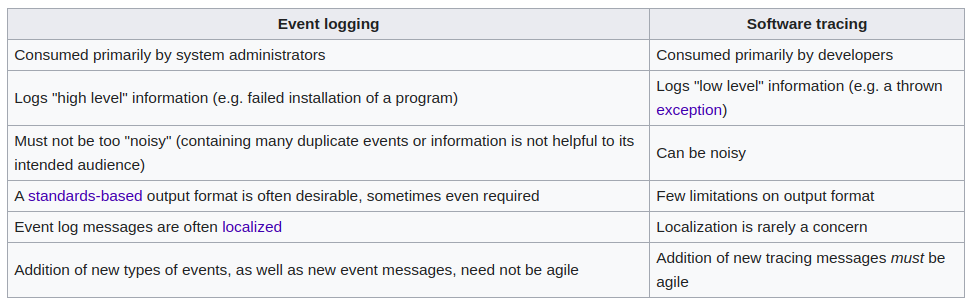
\includegraphics[width=120mm,height=60mm]{Slike/log_vs_trace.png}
    \end{center}
  \end{figure}

\section{Objasniti komentarisanje koda kao tehniku za prevenciju nastanaka bagova.}
  Komentarisanje je vid dokumentovanja koraka koji su doveli do toga da program izgleda
  kako izgleda. \\
  \noindent \textbf{Komentari moraju da opisuju:}
  \begin{itemize}
    \item Namenu nekog dela koda;
    \item Motivaciju da rešenje bude takvo kakvo je (posebno važno u slučaju naknadnog menjanja);
    \item Načine povezivanja sa drugim delovima koda (posebno način upotrebe potprograma).
  \end{itemize}
  \textbf{Komentari ne smeju da opisuju:}
  \begin{itemize}
    \item Ono što je očigledno;
    \item Ono što ne pripada konkretnom nivou apstrakcije.
  \end{itemize}

\section{Objasniti testiranje jedinica koda kao tehniku za prevenciju nastanaka bagova.}
  \noindent Pogledati pitanja: 
  \begin{itemize}
    \item Šta može biti jedinica koda koja se testira? 
          \ref{q_sta_moze_biti_jedinica_koda_koja_se_testira};
    \item Šta može biti predmet testiranja jedinice koda? 
          \ref{q_sta_moze_biti_predmet_testiranja_jedinice_koda}.
  \end{itemize}

\section{Navesti osnovne tehnike upotrebe debagera.}
  \begin{itemize}
    \item Izvršavanje korak po korak;
    \item Postavljanje tačaka prekida (breakpoint) u kodu ili podacima;
    \item Praćenje vrednosti promenljivih;
    \item Praćenje lokalnih promenljivih;
    \item Praćenje stanja steka;
    \item Praćenje na nivou instrukcija i stanja procesora.
  \end{itemize}

\section{Objasniti tehniku upotrebe debagera Izvršavanje korak po korak.}
  U izvršavanju korak po korak, korak može biti jedna linija izvornog koda ili jedna mašinska 
  instrukcija. Ukoliko naiđemo na tačku prekida pri izvršavanju koraka, izvršavanje programa će 
  stati na tačku prekida.

\section{Objasniti tehniku upotrebe debagera Postavljanje tačaka prekida.}
  Tačka prekida (eng. breakpoint) je lokacija u izvršnom kodu u kojoj operativni sistem staje 
  sa izvršavanjem i podiže debager. To nam omogućava da analiziramo situaciju i 
  prosledimo komande debageru (primer: provera vrednosti promenljivih u toj tački).

\section{Objasniti tehniku upotrebe debagera Praćenje vrednosti promenljivih.}
  Kucanjem \textit{info variables} u GDB-u možemo da pratimo imena i vrednosti svih globalnih i 
  statičkih promenljivih.

\section{Objasniti tehniku upotrebe debagera Praćenje lokalnih promenljivih.}
  Komandom \textit{info locals} u GDB-u možemo da pratimo imena i vrednosti svih lokalnih 
  promenljivih u stek okviru u kom se nalazimo, uključujući i statičke promenljive te funkcije.

\section{Objasniti tehniku upotrebe debagera Praćenje stanja steka.}
  Pri selektovanju stek okvira možemo pratiti imena i vrednosti 
  promenljivih koje su dostupne na tom steku. Komandom \textit{info args} možemo 
  da pratimo imena i vrednosti argumenata tog stek okvira.

\section{Objasniti tehniku upotrebe debagera Praćenje na nivou instrukcija i stanja procesora.}
  Neki debageri nam omogućavaju da pratimo instrukcije procesora. U okviru debagera GDB imamo komandu 
  \textit{(gdb) layout asm} koja prebacuje izgled TUI (text user interface) izgled u formu (isto TUI)
  koja prikazuje instrukcije procesora (registri, izvor, \dots). \cite{gdb_commands}

\section{Šta je dizajn softvera? Šta je arhitektura softvera? Objasniti sličnosti i razlike.}
  % \textbf{Dizajn softvera} je struktura softverskog sistema. Dizajn softvera je takođe disciplina
  % koja se bavi strukturom softverskog sistema i dokumentacija koja opisuje strukturu softverskog
  % sistema. \\ 
  % \indent \textbf{Arhitektura softvera} je struktura softverskog sistema, ali posmatrana
  % na relativno visokom nivou. Arhitektura softvera je takođe disciplina
  % koja se bavi strukturom softverskog sistema i dokumentacija koja opisuje strukturu softverskog
  % sistema. \\
  \indent Dizajn softvera i arhitektura softvera su strukture softverskog sistema. Razlika je u
  tome što je arhitektura softvera posmatrana na relativno visokom nivou. Arhitektura se odnosi više
  na spoljni deo softvera, tj. kako komponente komuniciraju međusobno i predstavlja apstrahciju 
  celog sistema. To znači da je svaka arhitektura softvera dizajn softvera, ali ne važi obrnuto.
  Neformalno rečeno, arhitekturu softvera ne zanima implementacija. \\

  ``Arhitektura predstavlja značajne odluke o dizajnu koje daju oblik sistemu, gde je značajnost
  određena cenom pravljenja izmena``
  \\[5pt]
  \rightline{{\rm --- Grady Booch, 2001}}\\

  Pri pravljenju arhitekture softverskog sistema preduzimaju se neke specifične aktivnosti i
  uzimaju u obzir specifični aspekti problema:
  \begin{itemize}
    \item Veliki značaj širine posmatranja;
    \item Manji značaj pojedinosti. 
  \end{itemize}

\section{Šta čini dizajn softvera? Navesti osnovne pojmove dizajna}
  \noindent \textbf{Elementi:}
  \begin{enumerate}
    \item komponente,
    \item implementacija,
    \item struktura podataka,
    \item infrastruktura,
    \item pomoćni alati,
    \item i sve drugo što je deo razvojnog procesa \dots
  \end{enumerate}
  \textbf{Osnovni pojmovi:}
  \begin{enumerate}
    \item \textbf{apstrahovanje}
    \item \textbf{dekompovanje}
  \end{enumerate}

\section{Šta je apstrakcija? Objasniti ulogu apstrakcije u dizajnu softvera.}
  \textbf{Apstrahovanje} je razmatranje opštih karakteristika problema i rešenja uz zanemarivanje
  pojedinosti. Podrazumeva rešavanje problema na konceptualnom nivou. Ima sličnosti sa
  mehanizmom indukcije: Posmatranjem specifičnih slučajeva se teži ka pravljenju opšteg modela.
  Za apstrakciju se može reći da je \textbf{uopšteno rešenje}.\\
  \indent Primer: Niz bitova na disku je datoteka.

\section{Šta je dekompozicija? Objasniti ulogu dekompozicije u dizajnu softvera.}
  \textbf{Dekompovanje} je postepeno preciziranje sistema kroz prepoznavanje manjih celina 
  (komponenti) koje ga čine. Rekurzivnom primenom dekompozicije se dolazi do fizičkog dizajna.
  Predstavlja vezu između različitih nivoa apstrakcije, gde se dekompozicijom apstraktnog
  sistema dolazi do njegove konkretne strukture. Ima sličnosti sa mehanizmom indukcije:
  Posmatranjem i razlaganjem opšteg slučaja se teži ka pravljenju konkretnijeg (preciznijeg)
  modela. Za dekompoziciju se može reći da je \textbf{razloženo rešenje}.\\
  \indent Primer: Jelovnik u restoranu se dekomponuje:
  \begin{itemize}
    \item jelovnik za glavno jelo;
    \item jelovnik za pića;
    \item jelovnik za dezert;
    \item ...
  \end{itemize}

\section{Navesti i ukratko objasniti 4 osnovna pojma dizajna softvera.}
  \begin{itemize}
    \item \textbf{Modularnost:} Složene celine se dele na manje module. Na višem nivou apstrakcije
          se posmatra celina, a na nižem dekompovani moduli koji čine celinu.
    \item \textbf{Enkapsulacija:} Razdvajanje posmatranja ponašanja komponenti i njihove
          implementacije. Na višem nivou apstrakcije se posmatra ponašanje, a na nižem
          implementacija.
    \item \textbf{Razdvajanje nadležnosti:} Jedan od osnovnih kriterijuma pri dekompoziciji. Svaka
          komponenta mora da ima jasno prepoznatu i zaokruženu odgovornost.
    \item \textbf{Interfejsi:} Predstavlja tačku vezivanja komponente. Može da se posmatra
          kao deklaracija ponašanja komponente.
  \end{itemize}

\section{Navesti i ukratko objasniti bar 6 ključnih principa dizajna softvera.}
  \begin{enumerate}
    \item \textbf{Princip jedinstvene odgovornosti:} Jedan modul bi trebalo da ima
          jednu namenu i samo jedan razlog za menjanje.
    \item \textbf{Razdvajanje odgovornosti:} Različite komponente bi trebalo da imaju različite
          odgovornosti. Nijedna odgovornost ne bi trebalo da bude podeljena na više odgovornosti.
    \item \textbf{Princip minimalnog znanja:} Jedna komponenta ne mora da zna kako druga funkcioniše.
          Dovoljno je da zna kako da je koristi.
    \item \textbf{Princip inverzne zavisnosti:} Apstrakcija ne sme da zavisi od pojedinosti, a
          pojedinosti moraju da zavise od apstrakcije, iako se u procesu projektovanja
          apstrakcija oblikuje na osnovu pojedinosti.
    \item \textbf{Princip acikličnih zavisnosti:} Izbegava se ciklična zavisnost komponenti.
          Složene zavisnosti otežavaju razumljivost i održavanje.
    \item \textbf{Princip stabilne zavisnosti:} Smer zavisnosti bi trebalo da se poklapa sa smerom
          porasta stabilnosti. Nije dobro da drugi moduli zavise od manje stabilnih modula.
    \item \textbf{Princip stabilne apstrakcije:} Modul bi trebalo da bude apstraktan koliko i stabilan.
          Drugi moduli bi trebalo da zavise od apstraktnih i stabilnih modula. 
    \item \textbf{Izbegavanje ponavljanja:} Nijedna funkcionalnost ne bi smela da se implementira
          više puta. Ako ima ponavljanja, to znači da rešenje nije dovoljno apstraktno.
    \item \textbf{Izbegavanje suvišnog posla:} Predvideti samo ono što je danas potrebno, a
          ono što će možda biti potrebno nije potrebno.
  \end{enumerate}

\section{Objasniti odnos pisanja koda i dizajniranja.}
  Pretpostavimo da je izvorni kod predstavlja dizajn softvera. Pisanje koda je u tom slučaju
  ekvivaletno dizajniranju. Tada je izgradnja (prevođenje) koda
  proces implementacije. Cena izgradnje je izuzetno niska (sve niža i niža sa bržim i jeftinijim
  računarima). Cena dizajniranja je relativno niska u odnosu na druge vrste projekata i dobijenu
  složenost. \\
  \indent \textbf{Problem:} Dizajn softvera lako i brzo postaje veoma složen. Programiranje je mnogo više
  od kodiranja. Programiranje obuhvata i projektovanje. \underline{Razvoj softvera je i zanatska
  i inžinjerska disciplina.} \\
  \textbf{Kako raditi?}
  \begin{itemize}
    \item \textbf{,,Projekat pre koda``:}
          \begin{itemize}
            \item Daje jasnu sliku projekta pre programiranja;
            \item Omogućava programerima da imaju jasniju sliku šta prave;
            \item Nudi jasnu i stabilnu sliku projekta;
            \item Često se menja tokom razvoja, čak i potpuno;
            \item Predstavlja ozbiljan, ali često neažuran vid dokumentacije.
          \end{itemize}
    \item \textbf{,,Projekat je kod``:}
          \begin{itemize}
            \item Iskusni programeri mogu da istovremeno prilagode i kod projektovanju i 
                  projekat načinu kodiranja;
            \item Štedi se vreme na projektovanju i može brže da se započne sa implementacijom
                  pojedinačnih modula.
            \item Može da dovodi do otežanog povezivanja komponenti;
            \item Ne postoji jasna slika projekta u ranim fazama razvoja.
          \end{itemize}
  \end{itemize} 

\section{Objasniti ulogu i mesto dizajniranja u razvoju softvera u savremenoj praksi.}
  \begin{itemize}
    \item \textbf{Što je dizajn nižeg nivoa, to se ređe pravi pre samog programskog koda:} Dizajn softvera se 
          sve ređe pravi i dokumentuje pre kodiranja. Ako se on pravi, onda je samo umereno
          detaljan. \\
    \item \textbf{Što je dizajn višeg nivoa, to je neophodno njegovo pažljivo planiranje 
          i dokumentovanje pre kodiranja:} Arhitektura softvera se najčešće pravi i dokumentuje pre kodiranja.
          Preskakanje arhitekture obično ima skupe posledice. \\
    \item \textbf{Granica između dizajna i arhitekture je obično nivo komponente:} Šta god to bilo u 
    konkretnom slučaju \dots
  \end{itemize}
  \textbf{Planiraju se:}
  \begin{itemize}
    \item komponente,
    \item njihovi interfejsi,
    \item njihovi međusobni odnosi.
  \end{itemize}
  To obično spada u arhitekturu. Ne planira se detaljno implementacija komponenti 
  (to obično spada u dizajn).\\
  \indent ,,Projektovanje`` se praktično izjednačava sa ,,oblikovanjem arhitekture``. Na taj način
  se izbegavaju problemi oba pristupa. Dobija se jasna velika slika dekompozicije sistema na 
  komponente i jasno se definišu njihovi interfejsi. Ne gubi se suviše vremena na projektovanje
  pojedinosti u ranim fazama razvoja, a koje će se kasnije često menjati. Što je sistem složeniji,
  to se arhitektura pravi na više različitih nivoa apstrakcije, tj. ,,projektovanje`` mora da se
  radi detaljnije.

\section{Navesti i ukratko objasniti obaveze softverskog arhitekte.}
  \begin{enumerate}
    \item \textbf{Razumevanje svih aspekata razvoja:} Odnosi se na poznavanje, planiranje i
          praćenje razvojnog procesa, i uzimanje u obzir sva praktična ograničenja.
    \item \textbf{Razumevanje sopstvene uloge:} Odnosi se na preuzimanje odgovornosti za ključne odluke
          bez zalaženja (iz ugla arhitekture) u nebitne detalje.
    \item \textbf{Komuniciranje sa ulagačima:} Arhitektura mora da zadovoljava potrebe ulagača.
    \item \textbf{Izvođenje rešenja iz poslovnih potreba:} Odnosi se na prepoznavanje i razumevanje
          potreba. Arhitektura je ,,slika`` poslovnog okruženja.
    \item \textbf{Uticanje na zahteve:} Odnosi se na prepoznavanje kompromisa i predočavanje
          ulagačima. Pomaganje ulagačima da donesu ispravne odluke.
    \item \textbf{Upravljanje rizicima i promenama:} Odnosi se na iterativno unapređenje i 
          prilagođavanje arhitekture.
    \item \textbf{Ponovljena upotreba:} Odnosi se na upotrebu postojećih dobara, čime se
          se štedi i novac.
    \item \textbf{Dobro odmeravanje učešća:} Arhitekta mora da donese odluke u svom domenu.
          Ne sme da izađe van svog domena. 
    \item \textbf{Preciziranje arhitekture prema tehnološkim ograničenjima:} Arhitektura se uvek
          implementira u nekom tehnološkom kontekstu.
    \item \textbf{Uvažavanje opštih okvira:} Svaka konkretna arhitektura je samo deo šireg
          poslovnog konteksta. Ona mora da se slaže sa ostalim elementima okruženja.
  \end{enumerate}

\section{Navesti i ukratko objasniti osnovne aspekte arhitekture i ključne uticaje na arhitekturu.}
  \noindent \textbf{Aspekti arhitekture:}
  \begin{itemize}
    \item \textbf{Šta?} Zahtevi koje softver mora da zadovolji.
    \item \textbf{Zašto?} Ključne odluke na osnovu kojih se oblikuje arhitektura.
    \item \textbf{Kako?} Komponente, interfejsi, odnosi. Na nižem nivou i dizajn i implementacija
          rešenja.
  \end{itemize}
  \textbf{Ključni uticaji (međusobno suprostavljene sile):}
  \begin{itemize}
    \item \textbf{Želje:} Sve ono što ulagači žele;
    \item \textbf{Izvodljivost:} Sve ono što tehnologija može da pruži;
    \item \textbf{Održivost:} Sve ono što u datim uslovima može da se postigne 
          (vreme, novac i drugi resursi);
    \item \textbf{Estetika:} Svi oni neformalni (iracionalni?) aspekti rešenja koji ga čine
          kvalitetnijim (nešto manje važna i jaka sila).
  \end{itemize}

\section{Prazno (radi usaglašavanja odgovora sa ispitnim pitanjima).}

\section{Šta su kohezija i spregnutost u kontekstu razvoja softvera?}
  \textbf{Kohezija (eng. cohesion)} je stepen međusobne povezanosti elemenata jednog modula.\\

  \textbf{Spregnutost (eng. coupling)} je stepen međusobne povezanosti elemenata dveju različitih
  modula. \\

  Dobro dizajniran softver se odlikuje visokom kohezijom i niskom spregnutošću komponenti.
  \cite{gfg_coupling_and_cohesion}
  \cite{sjsu_coupling_and_cohesion}

\section{Navesti vrste kohezije u kontekstu razvoja softvera.}
  \begin{itemize}
    \item funkcionalna (Functional)
    \item sekvencijalna (Sequential)
    \item komunikaciona (Communicational)
    \item proceduralna (Procedural)
    \item vremenska (Temporal)
    \item logicka (Logical)
    \item koincidentna (Coincidental)
  \end{itemize}
 
\section{Objasniti funkcionalnu koheziju u kontekstu razvoja softvera.}
  \textbf{Funkcionalna kohezija} predstavlja povezanost delova jednog modula na osnovu 
  međusobne funkcionalne zavisnosti u cilju ostvarivanja funkcije za koju je komponenta
  odgovorna. Svi delovi su prikupljeni sa jednim istim osnovnim ciljem. Svaki deo je potreban i
  nijedan deo nije višak. Predstavlja idealnu situaciju. \\
  \textbf{Napomena:} Sledeći primer i primeri koju slede se odnose na koheziju klasa. Ove primere
  možemo posmatrati kao analogiju, gde klase igraju ulogu modula, a komponente igraja ulogu
  metoda.

  \begin{lstlisting}
    class Plane
    {
    public:
        void takeoff();
        void fly();
        void land();
    };\end{lstlisting}

\section{Objasniti sekvencijalnu koheziju u kontekstu razvoja softvera.}
  Koehezija je \textbf{sekvencijalna kohezija} ako su elementi komponente projektovani 
  tako da izlaz jedne komponente predstavlja ulaz u drugu komponentu. Ne postoji puna
  funkcionalna zavisnost. Delovi sekvence potencijalno obavljaju različite poslove. Postoji
  potencijalno otvoren problem odgovornosti u odnosu na celovit posao. Ovaj tip kohezije
  se sasvim prirodno pojavljuje u funkcionalnim jezicima. Primer: protok podataka.
  
\section{Objasniti komunikacionu koheziju u kontekstu razvoja softvera.}
  Kohezija je \textbf{komunikaciona kohezija} ako su elementi komponente prikupljeni 
  zato što koriste iste podatke. Ne postoji funkcionalna zavisnost i delovi obično obavljaju
  različite poslove. Obično nisu dobro razdvojene odgovornosti: 
  \begin{itemize}
    \item Jedna komponenta ima više odgovornosti;
    \item Jedna komponenta je podeljena na više kompenenti.
  \end{itemize}
  Primer: Ažurira se slog u bazi podataka i šalje se pisaču.

\section{Objasniti proceduralnu koheziju u kontekstu razvoja softvera.}
  Kohezija je \textbf{proceduralna kohezija} ako su elementi komponenti prikupljeni zato što
  se koriste pri obavljanju nekog celovitog posla. Verovatno ne postoji funkcionalna
  zavisnost i komponente obavljaju potpuno raznorodne poslove (koji se obično obavljaju
  jedan za drugim). Obično nisu dobro razdvojene odgovornosti:
  \begin{itemize}
    \item Jedna komponenta ima više odgovornosti;
    \item Jedna odgovornost je podeljena na više komponenti.
  \end{itemize}
  Primer: Otvaranje datoteke, proveravanje ispravnosti, čitanje, ...\\
  Primer: Pravljenje torte :)

  \begin{lstlisting}
    class BakeCake
    {
    public:
        void addIngredients();
        void mix();
        void bake();
    };\end{lstlisting}

\section{Objasniti vremensku koheziju u kontekstu razvoja softvera.}
  Kohezija je \textbf{vremenska kohezija} ako su elementi komponente prikupljeni zajedno 
  zato što se koriste u ,,istom`` vremenskom periodu. Verovatno ne postoji funkcionalna zavisnost i
  često delovi obavljaju raznorodne poslove. Obično nisu dobro razdvojene odgovornosti: 
  \begin{itemize}
    \item Jedna komponenta ima više odgovornosti;
    \item Jedna komponenta je podeljena na više kompenenti.
  \end{itemize}
  Primer: Različiti elementi inicijalnog sistema. 

  \begin{lstlisting}
    class InitFuns
    {
    public:
        void initDisk();
        void initPrinter();
        void initMonitor();
    };\end{lstlisting}

\section{Objasniti logičku koheziju u kontekstu razvoja softvera.}
  Kohezija je \textbf{logička kohezija} ako su elementi komponente prikupljeni zajedno zato što
  imaju logički sličnu (ili čak istu) ulogu u sistemu. Najčešće ne postoji funkcionalna
  zavisnost i delovi najčešće obavljaju raznorodne poslove koji mogu predstavljati alternativu
  jedni drugima. Obično nisu dobro razdvojene odgovornosti: 
  \begin{itemize}
    \item Jedna komponenta ima više odgovornosti;
    \item Jedna komponenta je podeljena na više kompenenti.
  \end{itemize}
  Primer: Računanje površina različitih oblika.

  \begin{lstlisting}
    class AreaFuns
    {
    public:
        double circleArea();
        double rectangleArea();
        double triangleArea();
    };\end{lstlisting}

\section{Objasniti koincidentnu koheziju u kontekstu razvoja softvera.}
  Kohezija je \textbf{koincidentna kohezija} ako su elementi kohezije međusobno nespregnuti 
  ili su veoma slabo spregnuti. 
  Ne postoji nikakva (ili postoji sasvim niska) funkcionalna zavisnost. Delovi obavljaju raznorodne
  poslove i uopšte nisu razdvojene odgovornosti. Ovo je najniži nivo kohezije.
  Primer: Vraćanje datuma uz inicijalizaciju pisača.
  
  \begin{lstlisting}
    class MyFuns
    {
    public:
        void initPrinter();
        double calcInterest();
        Date getDate();
    };\end{lstlisting}

\section{Navesti osnovne karakteristike spregnutosti u kontekstu razvoja.}
  \begin{enumerate}
    \item vrsta sprege
    \item nivo sprege
    \item širina sprege
    \item način ostvarivanja sprege
    \item intenzitet spregnutosti
  \end{enumerate}

\section{Zašto je spregnutost komponenti softvera potencijalno problematična?}
  Da bi komponente sistema sarađivale, one moraju da budu spregnute. Ako komponente 
  komuniciraju ili sarađuju na bilo koji način, onda među njima postoji sprega. Ako
  su komponente potpuno nezavisne, onda one ne moraju da sarađuju. \\
  \indent Spregnutost nije problem sama po sebi. Problem mogu predstavljati neke karakteristike
  spregnutosti. \\
  \indent Želimo da umanjimo spregnutost da bismo mogli praviti izmene na jednom mestu bez toga
  da budemo time primorani da pravimo izmene i na drugim mestima. 

\section{Navesti i ukrakto objasniti vrste spregnutosti u kontekstu razvoja softvera.}
  \begin{itemize}
    \item sprega logike
    \item sprega tipova
    \item sprega specifikacije
  \end{itemize}

\section{Objasniti spregu logike u kontekstu razvoja softvera.}
  Ako komponente dele informacije ili pretpostavke jedna o drugoj, onda je u pitanju
  \textbf{sprega logike}. Primeri:
  \begin{itemize}
    \item Komponente obavljaju različite delove istog posla.
    \item Komponenta A pretpostavlja da implentacija metoda B::M(...) počiva na nekom
          konkretnom algoritmu. Primer: A i B implementiraju komplementarne algoritme
          (kodiranje/dekodiranje, pisanje/čitanje, ...).
    \item Komponente dele pretpostavke o nekim konkretnim podacima. Primer: 
          A zapisuje datoteku pod nekim imenom, a B je čita.
  \end{itemize}
  Sprega logike je visoko problematična i nepoželjna.

\section{Objasniti spregu tipova u kontekstu razvoja softvera.}
  \textbf{Sprega tipova} označava da jedna komponenta koristi neki tip definisan u okviru druge
  komponente. Može biti \textbf{određena} ako komponenta A pravi instance tipa B ili
  može biti \textbf{neodređena} ako komponenta A ne pravi instance tipa B (tj. može se u praksi
  dobijati na upotrebu instance podtipova). Primer: Komponenta A koristi klasu implementiranu
  u komponenti B. \\
  \indent Dobro implementirana sprega tipova ne predstavlja problem. Ovo posebno važi u slučaju
  kada je neodređena.

\section{Objasniti spregu specifikacije u kontekstu razvoja softvera.}
  \textbf{Sprega specifikacije} je još apstraktnija nego sprega tipova. Pretpostavlja se 
  da nije poznat tip koji se koristi već samo neke pretpostavke o njegovom interfejsu. Primeri:
  \begin{itemize}
    \item Upotreba parametarskog ili implicitnog polimorfizma;
    \item Upotreba referenci na metode objekata;
    \item Apstraktne bazne klase hijerarhija;
    \item Implementacija interfejsa.
  \end{itemize}
  Dobro implementirana sprega specifikacije ne predstavlja problem.

\section{Navesti i ukratko objasniti nivoe spregnutosti u kontekstu razvoja softvera.}
  Spregnutosti se dele po nivou apstraktnosti delova koji se dele (od najjače ka najslabijoj):
  \cite{gfg_coupling_and_cohesion}
  \begin{itemize}
    \item po sadržaju (Content Coupling)
    \item preko zajednickih delova (Common Coupling)
    \item spoljašnja spregnutost (External Coupling)
    \item preko kontrole (Control Coupling)
    \item preko markera (Stamp Coupling)
    \item preko podataka (Data Coupling)
    \item preko poruka 
  \end{itemize}
  
\section{Objasniti spregnutost po sadržaju u kontekstu razvoja softvera.}
  \textbf{Spregnutost po sadržaju} predstavlja otvoreno i neposredno korišćenje
  i/ili menjanje sadržaja jedne komponente od strane druge. \\
  Opšti primer:
\begin{lstlisting}
  ... A::metod(...)
  {
    ... objB->podatak ...
  }\end{lstlisting}
Konkretan primer:
\begin{lstlisting}
  class Pilot { ... };
  class Plane
  {
      double altitude, speed;
      friend class Pilot;
      // etc.
  };\end{lstlisting}

  \noindent \textbf{Problem:}
  \begin{itemize}
    \item Narušena je enkapsulacija;
    \item Dovedene su u pitanje odgovornosti komponenti;
    \item Veoma je teško održavati komponentu od čijih internih aspekata implementacije
          zavisi druga komponenta.
  \end{itemize} 
  Spregnutost po sadžaju je najjača i najnepoželjnija vrsta spregnutosti.

\section{Objasniti spregnutost preko zajedničkih delova u kontekstu razvoja softvera.}
  \textbf{Spregnutost preko zajedničkih delova} je na delu ako dve ili više komponenti
  neposredno pristupaju nekim podacima. \\
  Opšti primer:
\begin{lstlisting}
  struct ZajednickiDelovi {...};
  ... A::metod1(...){
    ... zajednickiDelovi->podatak ...
  }
  ... B::metod2(...){
    ... zajednickiDelovi->podatak ...
  }\end{lstlisting}
  \textbf{Problem:} 
  \begin{itemize}
    \item Razlikuje se od spregnutosti po sadržaju samo po tome što su deljeni podaci
          odvojeni od ponašanja i stavljeni na upotrebu drugim komponentama.
    \item Enkapsulacija samo načelno nije narušena, a zapravo nije ni uspostavljena.
    \item Ni odgovornosti nisu uspostavljene.
    \item Veoma je teško održavati ovako spregnute komponente.
  \end{itemize}
  Spregnutost preko zajedničkih delova je skoro jednako nepoželjna kao spregnutost
  po sadržaju.

\section{Objasniti spoljašnju spregnutost u kontekstu razvoja softvera.}
  \textbf{Spoljašnja spregnutost} je na delu ako više komponenti upotrebljava isti od spolja
nametnut koncept (interfejs, format podataka, komunikacioni kanal, ...). \\
Opšti primer:
\begin{lstlisting}
  ... A::metod1 {
    ...external::oper1(...);
    ...external::oper2(...);
  };
  ... B::metod2(...){
    ...external::oper3(...);
    ...external::oper4(...);
  }\end{lstlisting}
  \textbf{Problem:}
  \begin{itemize}
    \item \textbf{Često ponavljanje koda:} Ako se koncept izmeni, moraju se menjati sve komponente
          koje ga upotrebljavaju. 
    \item \textbf{Podeljene odgovornosti:} Poželjno je razmotriti učauravanje elemenata spoljašnjeg
          koncepta u novu komponentu (ili komponente), koju bi zatim koristile ovako spregnute 
          komponente.
  \end{itemize}
  Spoljašnja spregnutost je sasvim prihvatljiva ako su spoljašnji koncepti relativno stabilni
  i pouzdani. Primer: \underline{slika} implementira osnovne metode, a \underline{transformacije}
  implementiraju složene operacije nad slikama.
  
\section{Objasniti spregnutost preko kontrole u kontekstu razvoja softvera.}
  Spregnutost je \textbf{spregnutost preko kontrole} ako jedna komponenta ultimativno upravlja
  radom druge komponente. 
  \begin{itemize}
    \item Upravljana komponenta nije u stanju da funkcioniše bez spoljašnje kontrole ili 
    \item Upravljana komponenta očekuje sva ili neka upustva za rad po kojima zatim samostalno
          postupa. 
  \end{itemize} 
  U odnosu na spolašnju spregnutost, kontroler je jedina ili primarna tačka kontrole. \\
  Primer:
\begin{lstlisting}
class Kontrolisana {
  ...oper1(...);
  ...oper2(...);
  };
  ... Kontroler::metod(...){
    ...kontrolisana->oper1(...)...
    ...kontrolisana->oper2(...)...
  }\end{lstlisting}
  Primer: Kontrolisana klasa može da bude slika, a sve složene transformacije se implementiraju
  u drugoj klasi koja predstavlja kontroler.\\

  \textbf{Problem:} Potencijalno nejasna podela odgovornosti. Ako je kontroler odgovoran
  za viši nivo operacija, onda to mora biti njegova jedina odgovornost. Često takvo rešenje 
  ni po čemu nije bolje od integrisanih svih operacija u jedan isti modul, tj. u oba slučaja
  potencijalno imamo module sa suviše odgovornosti.\\
  \indent Spregnutost preko kontrole je relativno jaka, ali može biti veoma korisna u nekim
  slučajevima. \\Primer: Kontrolisana komponenta implementira elementarne postupke, a različite
  strategije obezbeđuju složene načine upravljanja radom komponente. \\
  \indent Primer sa slikom:
  Na nivou klasa može da bude dobro da se za svaku transformaciju pravi ova klasa. Na nivou 
  komponenti, sve transformacije se obično okupljaju u jednu komponentu.

\section{Objasniti spregnutost preko markera u kontekstu razvoja softvera.}
  Spregnutost je \textbf{spregnutost preko markera} ako više komponenti međusobno razmenjuje
  neku složenu strukturu podataka (marker) koju upotrebljavaju na različite načine. 
  \textbf{Napomena:} Ako neposredno koriste iste podatke, onda je u pitanju spregnutost
  preko zajedničkih kanala. \\
  Primer:
\begin{lstlisting}
  ...
  parser->fillRequest( request );
  environment->prepareRequest( request );
  processor->performTransaction( request );
  response = reporter->prepareReport( request );
  ...\end{lstlisting}
  \textbf{Problem:}
  \begin{itemize}
    \item Potencijalno otvoreno pitanje odgovornosti markera: Šta je njegova odgovornost?
          Zašto ne sve ili neke operacije?
    \item Marker praktično nije dovoljno enkapsuliran.
    \item Postoji opasnost od sukoba nadležnosti.
  \end{itemize}
  Slično kao u slučaju spregnutosti preko kontrole, u nekim slučajevima je ovakvo rešenje
  sasvim prihvatljivo:
  \begin{itemize}
    \item Ako marker nema složeno ponašanje;
    \item Ako marker nije spregnut na drugi način osim ovim putem;
    \item Ako postupak obrade u kome marker učestvuje nije stabilan ili 
          realno zavisi od više različitih komponenti.
  \end{itemize}

\section{Objasniti spregnutost preko podataka u kontekstu razvoja softvera.}
  Spregnutost je \textbf{spregnutost preko podataka} ako je jedna komponenta koristi interfejs
  druge komponente putem koga mu prenosi pojedinačne podatke. \\
  Primer:
\begin{lstlisting}
  ... simulacija::promenaSmera(...)
  {
    ...
    automobil->skreniLevo( 5 );
    ...
  }\end{lstlisting}
  \textbf{Problem:} Zavisnost na nivou interfejsa.\\
  Ovaj vid spregnutosti je među najnižim i sasvim prihvatlijv.\\

  Spregnutost je \textbf{spregnutost preko poruka} ako jedna komponenta koristi interfejs
  druge komponente putem koga mu ne prenosi nikakve podatke. Primer:
\begin{lstlisting}
  ... A::metod1(...) {
    ...
    transakcija->izvrsi();
    ...
  }\end{lstlisting}
  \textbf{Problem:} Zavisnost na nivou interfejsa.\\
  Ovaj vid spregnutosti je najniži i sasvim prihvatlijv.\\

\section{Objasniti pojam širina sprege u kontekstu razvoja softvera.}
  \textbf{Širina sprege} komponenti odgovara broju elemenata komponente A (objekata, podataka,
  metoda, poruka, ...) koje upotrebljava komponenta B. \\
  \noindent \textbf{Poželjno je da sprega bude što uža:}
  \begin{itemize}
    \item Uska sprega znači da su jasni i podela odgovornosti među komponentama i razlog njihove
          spregnutosti.
    \item Ako je sprega široka, to može da znači da:
          \begin{itemize}
            \item Odgovornosti između ove dve komponente nisu dovoljno diferencirane. Možda je 
                  moguće suziti spregu implementiranjem nekih složenih celina koda u okviru
                  komponente A.
            \item Odgovornosti komponente A su preširoke. Možda je potrebno podeliti komponentu
                  A na više delova.
          \end{itemize} 
  \end{itemize}

\section{Objasniti pojam smer sprege u kontekstu razvoja softvera}
  \noindent \textbf{Sprega može biti:}
  \begin{itemize}
    \item \textbf{Jednosmerna:} Komponenta A upotrebljava elemente komponente B, ali ne i
          obratno.
    \item \textbf{Dvosmerna:} Komponenta A upotrebljava elemente komponente B, ali i komponenta B
          upotrebljava elemente komponente A.
    \item \textbf{Cirkularna:} Ne postoji neposredno dvosmerna sprege dveju komponenti, ali 
          postoji tranzitivna cirkularna spregnutost više komponenti.
  \end{itemize}
  Poželjno je da sprega bude jednosmerna. Dvosmerna i cirkularna sprega značajno uvećavaju složenost
  sistema:
  \begin{itemize}
    \item Usložnjava se podela odgovornosti među komponentama;
    \item Dovodi se u pitanje enkapsulacija.
  \end{itemize}
  Ipak, nekada dvosmera ili cirkularna spregnutost može da značajno pojednostavi dizajn. Primer:
  Inverzija odgovornosti kod obrasca ,,Posetilac``.
  
\section{Objasniti pojam statička spregnutost u kontekstu razvoja softvera.}
  \textbf{Statička spregnutost} se ostvaruje pre izvršavanja programa i eksplicitno je iskazana
  u programskom kodu. Primeri:
  \begin{itemize}
    \item Nasleđivanje klase;
    \item Podatak klase A je objekat klase B;
    \item Argument metoda klase A je objekat klase B;
    \item U metodama klase A se pravi ili upotrebljava objekat klase B.
  \end{itemize}

\section{Objasniti pojam dinamička spregnutost u kontekstu razvoja softvera.}
  \textbf{Dinamička spregnutost} se ostvaraju u toku izvšavanja programa i nije eksplicitno
  iskazana kodom programa. Ovakva spregnutost može da zavisi od konfiguracije, ulaznih parametara
  i slično \dots \\ 
  \indent Primer: Ako klasa A sadrži referencu na klasu B (statički), konkretan objekat 
  (dinamički konfigurisan) može pripadati bilo kojoj klasi koja nasleđuje B.

\section{Objasniti odnos statičke i dinamičke spregnutosti u kontekstu razvoja softvera.}
  Statička sprega je jača i nepoželjnija od dinamičke sprege. 
  \begin{itemize}
    \item Deklaracija (interfejsa...) i implementacija neke statički spregnute komponente
          imaju neposrednog uticaja na implementaciju ostalih spregnutih komponenti.
    \item Promena dinamički spregnute komponente je lokalizovana tj. ako
          odgovara nasleđenom interfejsu, onda je sve u redu, a ako ne odgovara,
          onda je potrebno samo popraviti tu komponentu.
  \end{itemize}

\section{Objasniti pojam intenzitet spregnutosti u kontekstu razvoja softvera.}
  \textbf{Intenzitet spregnutosti} se može izraziti numerički na više načina. Primer:
  \begin{itemize}
    \item \textbf{Intenzitet spregnutosti dveju komponenti:}\\
          $coefSprege(A,B) = coefVrste(A,B) + coefNivoa(A,B) + ...$
    \item \textbf{Spregnutost jedne komponente sa sistemom:}\\
          $ coefSprege(A) = sum_{B}(coefSprege(A,B))$
    \item \textbf{Ukupna spregnutost sistema:}\\
          $coefSpregeSistema = sum_{A}(coefSprege(A))$
  \end{itemize} 

\section{Na koji način se može pristupiti merenju i računanju intenziteta spregnutosti?}
  Mera spregnutosti neke komponente sa sistemom se može izraziti na više načina:
  \begin{itemize}
    \item \textbf{Broj komponenti koje se referišu iz te komponente:} Broj elemenata drugih komponenti  
          koje referišu iz te komponente.
    \item \textbf{Broj komponenti iz kojih se referiše ta komponente:} Broj elemenata te komponente koje
          se referišu iz drugih komponenti
    \item \textbf{Karakteristike posmatranih sprega.}
    \item \dots
  \end{itemize}

\section{Navesti i objasniti dva osnovna pravila u vezi spregnutosti komponenti u 
         kontekstu razvoja softvera.}
  \textbf{,,Aksiome spregnutosti``:}
  \begin{itemize}
    \item Sto je komponenta složenija, to je važnije da bude što manje spregnuta.
    \item Spregu je poželjno uvoditi na što jednostavnijim komponentama.
  \end{itemize}
  
\section{Navesti nekoliko uobičajenih načina spregnutosti komponenti.}
  Neki oblici spregnutosti su relativno česti. 
  Mogu se prepoznati u uzorcima za projektovanje. Primeri:
  \begin{itemize}
    \item arhitektura klijent-server
    \item hijerarhija pripadnosti
    \item cirkularna spregnutost
    \item sprega putem intefejsa
    \item sprega putem parametara metoda
  \end{itemize}

\section{Objasniti karakteristike spregnutosti u slučaju arhitekture klijent-server.}
  \noindent Jedan od najčešćih i tipičnih oblika sprege:
  \begin{itemize}
    \item Komponenta server pruža usluge;
    \item Komponenta klijent koristi usluge.
  \end{itemize}
  \textbf{Karakteristike sprege:}
  \begin{itemize}
    \item Jednosmerna;
    \item Poželjno uska (server pruža samo jedan tip usluga);
    \item Nivo sprege je obično relativno nizak - preko poruka ili preko parametara;
    \item Sprega tipova ili specifikacija;
    \item Nizak intenzitet sprege preporučuje ovu vrstu sprege kao idealnu.
  \end{itemize}

\section{Objasniti karakteristike spregnutosti u slučaju hijerarhije pripadnosti.}
\noindent Relativno čest oblik sprege:
  \begin{itemize}
    \item Komponenta roditelj sadrži više dece koja obavljaju funkciju ili delove funkcije;
    \item Komponente deca obavljaju svaka svoj deo odgovornosti;
    \item Roditelj je odgovoran za koordinaciju.
  \end{itemize}
Primer: prozor - dekorateri.\\
\textbf{Karakteristike sprege:}
  \begin{itemize}
    \item Obično jednosmerna;
    \item Relativno uska;
    \item Nivo sprege je obično relativno nizak - preko poruka ili preko parametara;
    \item Sprega tipova ili specifikacija;
    \item Nivo se često može dalje spustiti, npr. primenom uzorka graditelj.
  \end{itemize}

\section{Objasniti karakteristike spregnutosti u slučaju cirkularne spregnutosti.}
\noindent Relativno čest oblik sprege:
  \begin{itemize}
    \item Komponenta roditelj sadrži više dece;
    \item Svako dete zna ko mu je roditelj i pristupa mu radi određenih poslova.
  \end{itemize}
  Primer: prozor-kontrole\\
  \textbf{Karakteristike sprege:}
  \begin{itemize}
    \item Dvosmerna;
    \item Potencijalno široka;
    \item Nivo sprega je obično relativno nizak - preko poruka ili preko parametara;
    \item Sprege tipova ili specifikacija;
    \item Nivo se često može dalje spustiti, npr. primenom zajedničkih nadtipova 
          i/ili uzorka graditelj.
  \end{itemize}

\section{Objasniti karakteristike spregnutosti u slučaju sprege putem interfejsa.}
  \noindent Tipičan oblik sprege u OO razvoju:
  \begin{itemize}
    \item Komponenta B deklarise (i implementira) interfejs;
    \item Komponenta A upotrebljava komponentu B posredstvom interfejsa.
  \end{itemize}
  \textbf{Karakteristike sprege:}
  \begin{itemize}
    \item Potencijalno jednosmerna;
    \item Širina zavisi od kvaliteta dizajna interfejsa;
    \item Nivo sprege je obično relativno nizak - preko poruka ili preko parametara;
    \item Sprega tipova ili specifikacije.
  \end{itemize}

\section{Objasniti karakteristike spregnutosti u slučaju sprege putem parametara metoda.}
  \noindent Čest oblik sprege u OO razvoju:
  \begin{itemize}
    \item Komponenta A deklarise metod koji kao parametar prima komponentu B;
    \item Komponenta BB, kao specijalizacija komponente B, se predaje na upotrebu komponenti 
          A kao parametar deklarisanoj metodi.
  \end{itemize}
  \textbf{Karakteristike sprege:}
  \begin{itemize}
    \item Potencijalno jednosmerna;
    \item Širina zavisi od kvaliteta dizajna interfejsa;
    \item Nivo sprege je obično preko metoda;
    \item Obično sprega tipova ili specifikacija.
  \end{itemize}

\section{Objasniti odnos koncepta klase i pojma kohezije u kontekstu OO razvoja softvera.}
  U kontekstu OO programiranja, kohezija klase predstavlja stepen međupovezanosti elemenata jedne klase:
  \begin{itemize}
    \item Ako je nizak nivo kohezije u klasi, to znači da klasa nije dobro podeljena:
          \begin{itemize}
            \item Ako postoji kohezija između nekih elemenata klase, ali ne svih, ili
            \item ako se prepoznaje više različitih skupove elemenata klase unutar kojih postoji snažna kohezija.
          \end{itemize}
    \item Moguće je da postoji problem prepoznavanja odgovornosti klase. 
    \item Klasu je možda potrebno podeliti na više klasa.
  \end{itemize}

\section{Objasniti odnos koncepta klase i pojma spregnutosti u kontekstu OO razvoja softvera.}
  U kontekstu OO programiranja, spregnutost predstavlja stepen međupovezanosti različitih klasa:
  \begin{itemize}
    \item Ako je visok nivo spregnutosti različitih klasa, 
          to ukazuje da odgovornosti nisu dobro podeljene među klasama;
    \item Možda je od više klasa potrebno napraviti jednu;
    \item Možda je potrebno drugačije podeliti odgovornosti među klasama.
  \end{itemize}

\section{Šta su arhitekture zasnovane na događajima?}
  Klasičan pristup razvoju softvera podrazumeva implementiranje algoritama 
  koji obavljaju određeni posao:
  \begin{itemize}
    \item Primenom metoda od vrha naniže određene celine problema se izdvajaju u potprograme,
    \item i dalje aspekti problema ostaju celina.
  \end{itemize}

  \noindent Primer: Program koji u petlji proverava da li je korisnik pritisnuo neki taster, a zatim pristupa 
  u skladu sa akcijom korisnika.\\
  
  \indent Kod arhitektura zasnovanih na događajima, eksplicitna komunikacija među 
  objektima se zamenjuje mehanizmom emitovanja događaja i distribuiranja zainteresovanim objektima.
  Primer:
  \begin{itemize}
    \item Program obaveštava OS da je zainteresovan da reaguje na pritisak tastera od strane korisnika;
    \item OS prepoznaje dogadaj i salje programu poruku;
    \item Program (odgovarajući objekat) reaguje na poruku.
  \end{itemize}

\section{Objasniti motivaciju za upotrebu arhitektura zasnovanih na događajima.}
  Arhitekture zasnovane na događajima spuštaju nivo međusobne zavisnosti objekata i tako smanjuju 
  ukupnu složenost sistema:
  \begin{itemize}
    \item Uobičajen je nivo spregnutosti putem parametara ili čak putem poruka;
    \item Uobičajena je dinamička sprega:
          \begin{itemize}
            \item Konfigurisanje odnosa među objektima u fazi izvršavanja programa,
            \item Konfigurisanje odnosa među objektima pri pravljenju objekata;
          \end{itemize}
    \item Smanjuje se ukupan intenzitet spregnutosti.
  \end{itemize}
  Cena smanjivanja ukupne složenosti primenom arhitektura zasnovanih na događajima može 
  biti uvećavanje lokalne složenosti:
  \begin{itemize}
    \item Komponente koje sarađuju u sistemu zasnovanom na događajima su 
          jednostavnije iz ugla složenosti koda;
    \item Njihove operacije su definisane apstraktnije pa mogu biti teže za razumevanje, 
          ako se posmatraju lokalno, bez razmatranja čitavog sistema.
  \end{itemize}
  
\section{Objasniti osnovne pojmove i koncepte arhitekture zasnovane na događajima.}
  \noindent \textbf{Događaj} je prepoznatljiv \underline{uslov} koji inicira obaveštenje.\\
  \textbf{Obaveštenje} je događajem iniciran \underline{signal} koji se šalje primaocu.\\
  \textbf{Posledice:} Ovakva arhitektura omogućava da se za mnoge složene probleme napravi 
  rešenje koje obezbeđuje najniži mogući (poznati?) intenzitet sprege. 
  Pored toga, postoje dodatni kvaliteti:
  \begin{itemize}
    \item Ako neki signali prestanu da budu značajni, može da prestane njihovo praćenje, 
          a da komponenta koja ih emituje pri tome ne mora da se menja;
    \item Ako je neke signale potrebno obraditi višestruko, 
          dovoljno je dodati nove slotove koji će ih prihvatiti, a da se komponente koje 
          emituju signale, kao i druge komponente koji već obrađuju te signale, ne moraju menjati.
  \end{itemize}

\section{Navesti i objasniti slojeve toka događaja kod arhitektura zasnovanih na događajima.}
  \begin{itemize}
    \item \textbf{Generator događaja:} objekat koji prepoznaje da je nastupio uslov koji 
          predstavlja neki definisan dogadaj;
    \item \textbf{Mašina za obradu događaja:} mesto na kome se prepoznaje nastali događaj 
          i odabire i pokreće odgovarajuća akcija (ili niz akcija);
    \item \textbf{Kanal događaja:} mehanizam putem koga se događaj prosleđuje od generatora 
          do mašine za obradu događaja;
    \item \textbf{Niz događaja:} upravljanih aktivnosti - mesto ispoljavanja događaja.
  \end{itemize}

\section{Objasniti osnovne koncepte primene arhitekture zasnovane na događajima u okviru biblioteke QT.}
  Biblioteku QT koristimo za upravljanje događajima. Osnovni model objekta u QT biblioteci je 
  \textbf{QObject}. Glavna karakteristika ovog modela je mogućnost komunikacije između objekata preko
  \underline{signala i slotova}. Da bi se koristili signali i slotovi potrebno je uključiti makro
  \textbf{Q\_OBJECT} u okviru QObject klase. Preporučuje se da se za sve klase koje nasleđuju QObject 
  doda Q\_OBJECT makro, nezavisno od toga da li zapravo koriste signala ili ne (neke funkcije mogu
  da imaju čudno ponašanje u suprotnom). 

\section{Objasniti koncept signala u kontekstu primene arhitekture
         zasnovane na dogadajima u okviru biblioteke QT.}
  \textbf{Signali} su metodi koji proizvode događaje. Deklarišu se u okviru sekcije \underline{signals}
  kao metodi tipa $void$ i ne implementiraju se. \\
  \indent Signali se emituju u obliku: emit signal(...). Ključna reč emit je makro. Za standardni C++ ima praznu 
  definiciju. Zato se može i izostavljati. Preporučuje se da se ne navodi radi kompatibilnosti koda, 
  dokumentovanja i lakšeg pronalaženja emitovanja.

\section{Objasniti koncept slotova u kontekstu primene arhitekture zasnovane na događajima u 
         okviru biblioteke QT.}
  \textbf{Slotovi} su metodi koji obrađuju događaje. Deklarišu se u okviru sekcije \textit{private slots}
  ili \textit{public slots}. Moraju biti istog tipa kao signali za čiju su obradu namenjeni.

\section{Objasniti povezivanje signala i slotova u slučaju primene arhitekture 
         zasnovane na događajima u okviru biblioteke QT.}
  Povezivanje se ostvaruje pomoću statičkog metoda QObject::connect. \\
  \textbf{Argumenti:}
  \begin{enumerate}
    \item Pokazivač na objekat koji emituje signal;
    \item Signal koji se emituje (navodi se pomocu makroa SIGNAL
          ili kao pokazivač na funkciju koja predstavlja signal);
    \item Pokazivač na objekat koji hvata signal;
    \item Slot kojim se signal hvata (navodi se pomoću makroa SLOT
          ili kao pokazivač na funkciju koja predstavlja slot).
  \end{enumerate}
  Slot i odgovarajući signal moraju biti istog tipa (nije važno ime).\\
  Zavisno od konfiguracije, nakon emitovanja signala se može sačekati i da se završi njegova obrada 
  ili odmah nastaviti sa radom. Podrazumevano ponašanje je da se sačeka sa obradom.\\
  Primer:
  \begin{lstlisting}
  Counter a, b;
  QObject::connect(&a, &Counter::valueChanged,
                    &b, &Counter::setValue);

  a.setValue(12);     // a.value() == 12, b.value() == 12
  b.setValue(48);     // a.value() == 12, b.value() == 48\end{lstlisting}
  Objašnjenje: Promena vrednosti objekta (brojača) $a$ predstavlja događaj koji emituje signal
  \textit{Counter::valueChanged}. Objekat $b$ hvata signal u okviru slota \textit{Counter::setValue}
  koji ažurira vrednost objekta $b$. Promena objekta $b$ ne utiče na objekat $a$, jer nije tako
  definisano preko statičke $connect$ metode.\\

  Koja je razlika između korišćenja makroa SIGNAL i SLOT i korišćenja pokazivača
  na funkcije? Pre QT verzije 5 je postojao samo prvi način (makroa). Od QT verzije 5 moguće
  je koristiti i drugu varijantu.
  
\section{Objasniti odnos arhitektura zasnovanih na događajima i problema kohezije i spregnutosti.}
  \noindent Sprega preko signala i slotova je dinamička sprega:
  \begin{itemize}
    \item Objekti koji se povezuju nisu spregnuti u kodu kojim su definisani;
    \item Sprega se uspostavlja u posebnom konfiguracionom delu programskog koda.
  \end{itemize}
  Ipak, uspostavljanje sprege (tj. povezivanje slotova i signala) je implementirano na statički način:
  \begin{itemize}
    \item Veze se uspostavljaju jednokratno;
    \item Veze između signala i slotova se uspostavljaju bezuslovno.
  \end{itemize}
  Uspostavljanje sprege putem povezivanja signala i slotova može da bude implementirano 
  i na dinamički način:
  \begin{itemize}
    \item Veze se mogu predstavljati u zavisnosti od konteksta;
    \item Tokom izvršavanja programa se veze mogu raskidati i ponovo uspostavljati;
    \item Metod QObject::disconnect.
  \end{itemize}
  
  Naredni korak bi bilo dinamičko programsko pravljenje slotova i signala 
  i zatim njihovo povezivanje. Biblioteka Qt nema neposrednu podršku za dinamičko 
  pravljenje slotova i signala, ali postoji više primera dodatnih klasa koje to omogućavaju.\\
  \indent Moguće primene su u implementaciji skript jezika, dinamičkih okruženja za pravljenje ili 
  menjanje korisničkih intefejsa i slično.
  
\section{Šta je konkurento izvršavanje?}
  Dva posla T1 i T2 se izvršavaju konkurentno ako nije unapred poznata njihova međusobna 
  vremenska lociranost. Primeri:
  \begin{enumerate}
    \item Posao T1 može da počne i završi pre početka T2.
    \item Posao T1 može da počne i završi posle započinjanja posla T2.
    \item Posao T1 može da počne pre započinjanja posla T2 i završi posle završavanja posla T1.
    \item Posao T1 može da počne posle započinjanja posla T2 i završi pre završavanja posla T2.
  \end{enumerate}
  
\section{Objasniti pojam paralelno izvršavanje.}
  Dva posla se izvršavaju paralelno ako postoji period vremena u kome su (doslovno) 
  istovremeno aktivni. Paralelno izvršavanje je moguće samo ako imamo na raspolaganju
  više izvršnih jedinica (procesora ili jezgara). \\
  
  \begin{figure}[H]
    \begin{center}
        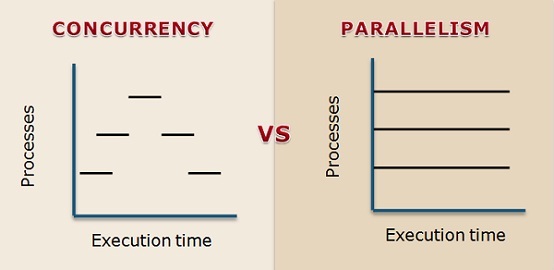
\includegraphics[width=80mm,height=50mm]{Slike/konkurencija_paralelizacija.jpg}
    \end{center}
  \end{figure}

  \noindent \textbf{Razlika i sličnosti između konkurentnog i paralelnog izvršavanja:}
  \begin{enumerate}
    \item Konkurentnost podrazumeva neodređenost vremenskog odnosa, a paralelnost podrazumeva
          predodređenost vremenskog odnosa.
    \item Konkurentni programi u krajnjem ishodu mogu da rade sekvencijalno ili deo po deo
          sekvencijalno, a paralelni programi moraju da rade istovremeno.
    \item Konkurentni poslovi mogu, ali ne moraju da se izvršavaju paralelno. Paralelni poslovi
          mogu, ali ne moraju da budu konkurentni. Paralelni poslovi nisu konkurentni ako je unapred
          poznata njihova međusobna vremenska lociranost tokom čitavog perioda izvšavanja.
    \item Programi su konkurentni ako su istovremeno u stanju izvršavanja. Programi su paralelni
          ako se istovremeno izvršavaju. 
    \item Konkurentno izvršavanje je moguće i na jednoj izvršnoj jedinici (procesoru). 
          Paralelno programiranje zahteva više izvršnih jedinica (procesora ili jezgara).
  \end{enumerate}

  \textbf{Motivacija:} Paralelizacija, tj. podela posla na procese/niti, 
  se preduzima iz dva osnovna razloga:
  \begin{itemize}
    \item \textbf{Razdvajanje odgovornosti:}
      \begin{itemize}
        \item Omogućava da potpuno razdvojimo kod koji radi jedan celovit deo posla;
        \item Primer: Jedna nit komunicira sa korisnikom i pravi zadatke, druga nit izvršava, 
              a treća asinhrono prikazuje dokle se stiglo sa izvršavanjem poslova;
        \item Često različiti procesi/niti imaju uloge klijenata ili servera u odnosu na druge 
              niti/procese;
        \item Poslovi se mogu dodatno razdvojiti tako da se izvršavaju na različitim računarima 
              (distribuirano izvršavanje);
        \item Iako može da izgleda kao podizanje složenosti, razdvajanje odgovornosti na procese/niti 
              je često prirodniji način rešavanja problema i zapravi ima nižu složenost nego 
              veštačko spajanje u jedan postupak.
      \end{itemize}
    \item \textbf{Podizanje performansi:}
      \begin{itemize}
        \item Ako je potrebno da se neki posao uradi nad velikom količinom podataka, 
              a na raspolaganju je više procesora, onda se efikasnost može višestruko uvećati 
              podelom posla na više procesa/niti, od kojih svaki radi nad delom podataka;
        \item Primer: Ako je potrebno primeniti neku lokalnu transformaciju slike, onda se slika može 
              podeliti na oblasti i obrada svake od oblasti poveriti drugom procesoru;
        \item Takva podela često nije sasvim prirodna i podiže složenost arhitekture;
        \item U takvim slučajevima se često ubraja u optimizacije.
      \end{itemize}
  \end{itemize}

\section{Objasniti pojam distribuirano izvršavanje.}
  Dva posla se izvršavaju distribuirano ako rade na različitim adresnim prostorima.
  Ovo je opštija definicija, koja teži da izjednači (apstrahuje) distribuiranost između 
  više računara i distribuiranost između komponenti (procesora) istog računarskog sistema.
  Neke definicije su strože i podrazumevaju različite računarske sisteme, ali 
  svi aspekti distribuiranja su uglavnom isti.
  
\section{Objasniti pojam proces.}
  \textbf{Proces} je instanca programa koja se izvršava na računarskom sistemu. 
  Obično se razmatra samo u kontekstu računarskih sistema koji imaju mogućnost 
  izvršavanja više programa (ili instanci programa) u ,,isto`` vreme. Ranije je definicija 
  podrazumevala da se proces izvršava sekvencijalno, ali to više nije tako.\\
  \textbf{Proces obuhvata:}
  \begin{enumerate}
    \item Kod programa koji se izvršava;
    \item Tekuće stanje procesa.
  \end{enumerate}
  \textbf{Stanje procesa obuhvata:}
  \begin{itemize}
    \item Podatke o izvršavanju;
    \item Stanje izvršavanja (primer: spreman, radi, čeka, stoji, ...);
    \item Brojač instrukcija (adresa naredne instrukcije);
    \item Sačuvane vrednosti registara procesora;
    \item Informacije o upravljanju resursima;
    \item Informacije o memoriji (tablica stranica, podaci o alokaciji memorije, ...);
    \item Deskriptori datoteka;
    \item Ostali resursi, poput U/I zahteva i sličnog.
  \end{itemize}
  
  \textbf{Promena konteksta (eng. context switch)} je promena stanja procesora koja je 
  neophodna u slučaju kada procesor sa izvršavanja koda jednog procesa prelazi 
  na izvršavanje koda drugog procesa. Stanje prethodno izvršavanog procesa zapisuje u memoriji. 
  Stanje narednog procesa koji će se izvršavati se čita iz memorije.\\
  \textbf{Cena procesa:}
  \begin{itemize}
    \item Procesi su dvojako skupi;
    \item Promena konteksta uzima značajno vreme procesora;
    \item Promena konteksta se dešava veoma često (od nekoliko puta do nekoliko hiljada 
          puta u sekundi);
    \item Veliki broj procesa može da oslabi performanse;
    \item Podaci o stanju procesa su obimni, zauzimaju mnogo memorije i pri svakoj promeni konteksta 
          se promašuju u kešu.
  \end{itemize}

\section{Objasniti pojam nit.}
  \textbf{Nit izvršavanja} je komponenta koja se izvršava sekvencijalno. Jedan proces može imati više 
  niti, ako računarski sistem to podržava. Svaki proces započinje sa jednom glavnom niti.
  Nit je najmanja samostalna jedinica izvršavanja na procesoru.

  \begin{figure}[H]
    \begin{center}
        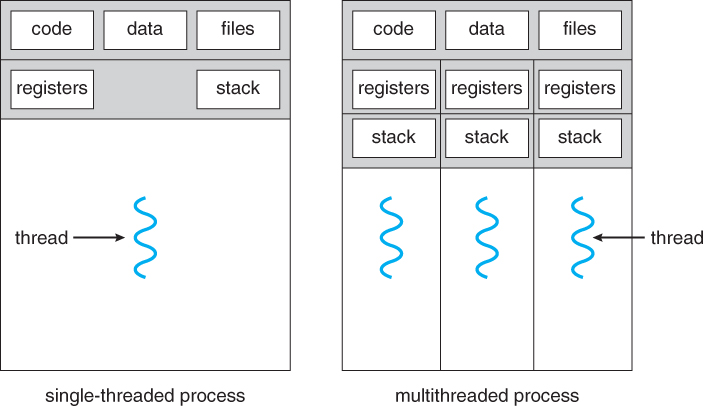
\includegraphics[width=80mm,height=50mm]{Slike/proces_niti.jpg}
    \end{center}
  \end{figure}

  \textbf{Stanje procesa i niti:}
  \begin{itemize}
    \item Podaci koji se vode na nivou procesa i zajednički su za sve niti tog procesa obuhvataju:
      \begin{itemize}
        \item Kod programa koji se izvršava;
        \item Informacije o upravljanju resursima;
        \item Informacije o memoriji (tablica stranica, podaci o alokaciji memorije, ...);
        \item Deskriptori datoteka;
        \item Stanje izvršavanja procesa;
        \item Ostali resursi, poput U/I zahteva i sl.
      \end{itemize}
    \item Podaci o niti obuhvataju:
      \begin{itemize}
        \item Stanje izvršavanja niti;
        \item Brojac instrukcija;
        \item Sačuvane vrednosti registara procesora.
      \end{itemize}
  \end{itemize}

\section{Zašto se uvodi koncept niti, ako već postoji koncept procesa?}
  Koncept niti izvršavanja koda se uvodi kako bi se spustila cena promena konteksta. 
  Jednom procesu može da odgovara više niti izvršavanja. Ako se većina podataka vodi na nivou i deli 
  među nitima jednog procesa, štedi se na resursima i dobija na performansama.

\section{Objasniti sličnosti i razlike niti i procesa.}
  \begin{enumerate}
    \item I procesi i niti se mogu izvršavati konkurentno i/ili paralelno;
    \item Značajan broj problema pri konkurentnom izvršavanju se odnosi na isti način 
          i na procese i na niti;
    \item Samo procesi se mogu izračunavati distribuirano;
    \item Sve niti jednog procesa rade istom adresnom prostoru;
    \item Procesi ne dele među sobom resurse (bar ne neposredno);
    \item Komunikacija između procesa se odvija isključivo kroz posebne mehanizme za 
          međuprocesnu komunikaciju;
    \item Nije potrebno eksplicitno staranje o eventualnom sukobljavanju oko resursa;
    \item Niti jednog procesa dele resurse tog procesa;
    \item Komunikacija između niti se najčešce odvija posredstvom deljenih resursa;
    \item Neophodno je eksplicitno staranje o eventualnom sukobljavanjem oko resursa.
  \end{enumerate}
  
\section{Objasniti kako se programiraju niti pomoću standardne biblioteke C++-a. Klase, metodi, \dots}
  \textbf{Klasa thread} je implementirana u okviru C++ modula \textit{thread}. Konstruktor za
  \textit{thread} prima pokazivač na funkciju (ime funkcije) i redom njene parametre. Nit se automatski
  pravi i pokreće (ne postoji metod za započinjanje). \cite{cppref_thread} \\
  \textbf{Osnovni metodi:}
  \begin{itemize}
    \item \textit{get\_id()} - Vraća identifikator niti;
    \item \textit{joinable()} - Provera se da li je nit spojiva;
    \item \textit{join()} - Spaja nit.
  \end{itemize}
  \textbf{Primer:}
\begin{lstlisting}
  #include <iostream>
  #include <thread>
   
  void some_function() 
  {
    // ...
  }
  
  void another_function(int x)
  {
    // ...
  }
  
  int main() 
  {
    // kreira se objekat thread koji poziva some_function()
    std::thread first (some_function);   
    // kreira se objekat thread koji poziva another_function(0)  
    std::thread second (another_function, 0);  
  
    std::cout << "main, both functions now execute concurrently...\n";
  
    // sinhronizacija niti:
    // ceka se da prva nit zavrsi
    first.join();        
    // ceka se da druga nit zavrsi        
    second.join();              
  
    std::cout << "both functions completed.\n";
  
    return 0;
  }\end{lstlisting}

\section{Objasniti kako se programiraju niti pomoću biblioteke QT. Klase, metodi, ...}
  \noindent Osnovnu podrške predstavlja klasa QThread. \\
  \textbf{Osnovni metodi:}
  \begin{itemize}
    \item \textit{bool isFinished()}
    \item \textit{bool isRunning()}
    \item \textit{bool wait(unsigned long time msec = ULONG\_MAX)}
  \end{itemize}
  \textbf{Slotovi (mogu se koristiti kao metodi):}
  \begin{itemize}
    \item \textit{void start()}
    \item \textit{void quit()}
    \item \textit{void terminate()}
  \end{itemize}
  \textbf{Signali:}
  \begin{itemize}
    \item \textit{void finished()}
    \item \textit{void started()}
    \item \textit{void terminated()}
  \end{itemize}
  Nova klasa niti nasleđuje klasu QThread implementira se zastićeni metod void \textit{run()}.\\
\begin{lstlisting}
  #include <QThread>

  class MyThread : public QThread {
  
    Q_OBJECT
  
  public:
  
    MyThread(...);
  
  protected:
  
    void run();
  
  };\end{lstlisting}
  
\section{Navesti i ukratko objasniti osnovne operacije sa nitima.}
  \noindent \textbf{Pravljenje:}
    \begin{itemize}
      \item Pravljenje niti na nivou OS-a obično podrazumeva i započinjanje njenog izvršavanja;
      \item Pravljenje objekta niti QThread ne podrazumeva i pravljenje niti na nivou OS-a;
      \item Nit će biti napravljena na nivou OS-a tek kad se pozove metod start().
    \end{itemize}
  \textbf{Dovršavanje:}
    \begin{itemize}
      \item Kada nit završi svoje izvršavanje, oslobađa se većina resursa vezanih za nit;
      \item Ostaje samo konačan status niti (rezultat izvršavanja, slično funkciji main).
    \end{itemize}
  \textbf{Suspendovanje i nastavljanje:}
    \begin{itemize}
      \item Neki OS omogućavaju da se nit privremeno suspenduje i da se kasnije njeno 
            izvršavanje nastavi (Windows, Solaris);
      \item Kod OS koji ne podržavaju suspendovanje, odgovarajuće ponašanje se može ostvariti 
            samo složenijim mehanizmima za sinhronizaciju:
            \begin{itemize}
              \item Razlozi za višestruki, ali se sumiraju u potencijalno nekontrolisanom držanju 
                    zaključanih resursa od strane suspendovane niti;
              \item POSIX.
            \end{itemize}
    \end{itemize}
  \textbf{Prekidanje:}
    \begin{itemize}
      \item Jedna nit može da prekine izvršavanje druge niti;
      \item Iako se ostvaruje naizgled jednostavno (pozivom jedne funkcije OS-a) 
            ovo je veoma osetljiva operacija;
      \item Prekidanje niti preti da ugrozi konzistentnost deljenih podataka.
    \end{itemize}
  \textbf{Čekanje:}
    \begin{itemize}  
      \item Elementaran vid sinhronizovanja niti je kada jedna nit čeka da druga završi sa radom;
      \item Ostvarivanje čekanja je relativno jednostavno, ali se preporučuje implementacija 
            složenijih mehanizama;
      \item Primer: Nit koja završava može da postavlja neki deljeni signal, koji se zatim može 
            lako proveravati od strane drugih niti.
    \end{itemize}
    \textbf{POSIX (Portable Operating System Interface)} je familija standarda definisana od strane
    IEEE ogranizacije sa namenom da se održi odgovarajuća kompatabilnost između operativnih sistema.

\section{Objasniti detaljno operaciju pravljenja niti. Kako se implementira pomoću 
         standardne biblioteke C++-a?}
  Pogledati prethodno pitanje sa primerom: 
  ,,Objasniti kako se programiraju niti pomoću standardne biblioteke C++-a. Klase, metodi, \dots``

\section{Objasniti detaljno operaciju pravljenja niti. 
         Kako se implementira pomocu biblioteke QT?}
  Objekat klase QThread predstavlja pomoćno sredstvo za rukovanje nitima OS-a. 
  Konstrukcija objekata ne obuhvata pravljenje niti. Nova nit se zaista pravi (na nivou OS-a) 
  kada se pozove metod void \textit{start()} objekta klase QThread.\\

  \textbf{Napomena:} Prilikom pokretanja niti se koristi metoda \textit{start()}, a ne 
  metoda \textit{run()} koja se implementira u okviru klase koja nasleđuje QThread klasu.
  Prilikom pokretanja niti preko \textit{start()} se kreira nit sa svojom memorijom i kodom, a onda se 
  u okviru \textit{start()} metode poziva metoda \textit{run}.
  
\section{Objasniti detaljno operaciju dovršavanja niti. Kako se implementira pomoću standardne
         biblioteke C++-a?}
  Nit se dovršava kada završi izvršavanje ,,glavne`` funkcije niti. Objekat niti se dovršava kad se 
  izađe iz opsega u kojem je inicijalizovan. \\
  \indent Ako je nit spojiva (\textit{joinable() == true}), poziva se \textit{terminate()}.
  \cite{cppref_threaddestructor}

\section{Objasniti detaljno operaciju dovršavanja niti. Kako se implementira pomocu biblioteke QT?}
  \begin{itemize}
    \item Nit se dovršava kada se završi izvršavanje metoda void run() objekta klase QThread.
    \item Postoji metod \textit{QThread::quit()} koji predstavlja opciju za dovršavanje niti.
          Ovaj metod ne radi ništa ako nit nema petlju za proveru događaja ili neki deo koda
          blokira petlju za proveru događaja.
    \item Postoji metod \textit{QThread::terminate()}, ali korišćenje ove metode je loša
          praksa.
  \end{itemize}
  

\section{Objasniti detaljno operacije suspendovanja i nastavljanja niti. Kako se implementiraju
         standardne biblioteke C++-a?}
  Standardna biblioteka C++ nam nudi opciju da suspendujemo nit (u smislu da oslobodi CPU),
  kako bi se dao prioritet drugim nitima. Ovo se izvodi preko funkcije \textit{void yield()}
  ili \textit{sleep()}. \cite{cppref_yield} 
  
\section{Objasniti detaljno operaciju suspendovanja i nastavljanja niti. 
         Kako se implementira pomocu biblioteke QT?}
  Suspendovanje niti nije moguće u QT.
  
\section{Objasniti detaljno operaciju prekidanja niti. Kako se implementira pomoću standardne
         biblioteke C++-a?}
  \begin{itemize}
    \item Nit se može prekinuti pozivanjem \textit{terminate()} preko neke druge niti i nit
          na koja je referisana će biti prisilno prekinuta;
    \item Može da se pozove deskruktor niti \textbf{\textasciitilde thread()}. 
  \end{itemize}

\section{Objasniti detaljno operaciju prekidanje niti. Kako se implementira pomoću biblioteke QT?}
  Nit se može prekinuti pozivanjem metoda void \textit{terminate()}. 
  Nit ne mora biti prekinuta tokom izvršavanja metoda.
  Kada će stvarno nit biti prekinuta zavisi od odgovarajuće politike OS-a.
  Ako je potrebno da se nit pouzdano završi, nakon pozivanja ovog metoda se može sačekati 
  da se niti završi.
  
\section{Objasniti detaljno operaciju čekanja niti. Kako se implementira pomoću standardne
         biblioteke C++-a?}
  Elementaran vid sinhronizovanja niti je kada jedna nit čeka da druga nit završi sa radom. \\

  Ostvarivanje čekanja je relativno jednostavno, ali se preporučuje implementacija složenih
  mehanizama (primer: nit koja završava može da postavlja neki deljeni signal, koji je se zatim
  može lako proveriti od strane drugih niti). \\

  Čekanje da se nit završi se izvodi pozivanjem metoda \textit{void join()}. Metod \textit{join()}
  završava rad tek kada odgavarajuća nit završi izvršavanje. Napomena: Na istoj niti se ne sme 
  pozvati dva puta metod \textit{join()}. 

\section{Objasniti detaljno operaciju čekanja niti. Kako se implementira pomoću biblioteke QT?}
  Biblioteka QT nema \textit{join()} metodu za niti. Ali metoda \textit{wait()} vrši sličnu
  funkciju. Nit se može čekati pozivanjem metoda bool \textit{wait(unsigned long time = ULONG\_MAX)}. 
  Ako se argument ne navede (ili se navede ULONG\_MAX), metod čeka dok se nit ne završi. 
  Inače, metod čeka na završavanje niti najviše \textit{time} milisekundi. 
  Metod vraća \textit{true} ako nit više nije aktivna (ili je završena ili nije ni započela rad) 
  i \textit{false} ako je nit jos aktivna.

\section{Koji su najvažniji problemi pri pisanju konkurentnih programa?}
  \begin{itemize}
    \item Deljenje resursa između jedinica izvršavanja;
    \item Komunikacija među jedinicama izvršavanja;
    \item Sinhronizacija jedinica izvršavanja.
  \end{itemize}
  
\section{Šta je muteks? Kako se upotrebljava?}
  \textbf{Muteksi (eng. mutex)} su jedan od osnovnih načina bezbednog deljenja podataka u 
  konkurentim okruženjima. Muteks ima sematiku katanca:
    \begin{itemize}
      \item Samo jedanput se može zaključati;
      \item Ako je muteks već zaključan, pokušaj zaključavanja će čekati na njegovo 
            otključavanja da bi se on mogao zaključati.
    \end{itemize}
  Implementiraju se (u osnovi) u okviru OS-a tako da operacije sa muteksima budu atomične.

\section{Objasniti podršku za mutekse u okviru standardne biblioteke C++-a.}
  Muteksi nude veoma jednostavan interfejs za signaliziranje 
  ekskluzivnog pristupa kod kritičnih sekcija (onemugućava pristup ostalim nitima).\\
  \textbf{Osnovne operacije:}
  \begin{itemize}
    \item \textbf{void lock():} Zaključava muteks ako je otklučan ili blokira izvršavanja.
    \item \textbf{bool try\_lock():} Ako je muteks otključan, onda ga zaključava i vraća
          true, u suprotnom vraća false. Može da se koristi da nit radi jedan posao
          koji zahteva kritičnu sekciju, ako je muteks otključan ili da radi drugi posao
          koji ne zahteva kritičnu sekciju, ako je muteks zaključan.
    \item \textbf{void unlock():} Otključava muteks. Ako je muteks već otključan, onda nije
          definisano ponašanje.
  \end{itemize}\cite{cppref_mutex}

  \section{Objasniti podrsku za mutekse u okviru biblioteke QT.}
  Muteksi su implementirani klasom \textbf{QMutex}. \\
  \noindent \textbf{Osnovni metodi:}
  \begin{itemize}
    \item \textbf{Zaključavanje muteksa:} \textit{void lock()}. Ako je već zaključan, 
          čeka da se otključa pa ga zaključava. U svakom slučaju, vraća se tek kada je 
          uspešno zaključan.
    \item \textbf{Otključava muteks:} \textit{void unlock()}. Otključava muteks. Ako je zaključan 
          od strane iste niti, otključa ga. Ako je zaključan od strane druge niti, proizvodi grešku.
          Ako nije zaključan ponašanje je nedefinisano.
    \item \textbf{Pokušaj zaključavanja:} \textit{bool tryLock()} Ako je muteks otključan, 
          zaključava ga i vraca \textit{true}. Ako je već zaključan, ne radi nista 
          i odmah vraca \textit{false}. Opcioni argument je maksimalno trajanje čekanja u ms
    \item \textbf{Konstruktor QMutex (RecursionMode mode = NonRecursive):} Opcioni argument može 
          da bude \textit{Qmutex::Recursive}. Tada jedna nit može da zaključa muteks više puta 
          uzastopno. Mora da ga otključa onoliko puta koliko ga je puta zaključala.
  \end{itemize}

  \textbf{Upotreba:} Uobičajeno je da se jednim muteksom obezbeđuje jedan podatak ili skup podataka 
  koji u jednom trenutku sme da upotrebljava samo jedna nit. Na početku atomičnog postupka muteks 
  se zaključava, a na kraju atomičnog postupka se otključava. Veoma je važno da se svaki 
  zaključani muteks otključa. Ako jedan isti muteks zaključava različite podatke, onda se 
  potencijalno spušta nivo konkurentnosti. Ako više muteksa zaključava jedan isti podatak, 
  otvara se prostor za ozbiljne previde u upravljanju tim resursom.


\section{Šta je, čemu služi i kako se koristi lock\_guard iz standardne biblioteke C++-a? 
         Objasniti detaljno.}
  \textbf{Klasa lock\_guard} je okvir za muteks koji nudi pogodan RAII mehanizam za postavljanje
  vlasništva nad muteksom u okviru definisanog bloka. Kada se \textit{lock\_guard} kreira,
  on pokušava da zauzme vlasništvo nad tim muteksom. Kada se izađe iz odgovarajućeg bloka, 
  \textit{lock\_guard} poziva svoj destruktor i muteks se oslobađa. \cite{cppref_lockguard}

\begin{lstlisting}
  #include <thread>
  #include <mutex>
  #include <iostream>
   
  int g_i = 0;
  std::mutex g_i_mutex; 
   
  void safe_increment()
  {
      const std::lock_guard<std::mutex> lock(g_i_mutex);
      ++g_i;
   
      std::cout << std::this_thread::get_id() << ": " << g_i << '\n';
   
      // g_i_mutex se automatski oslobadja kada
      // izadje iz opsega
  }
   
  int main()
  {
      std::cout << "main: " << g_i << '\n';
   
      std::thread t1(safe_increment);
      std::thread t2(safe_increment);
   
      t1.join();
      t2.join();
   
      std::cout << "main: " << g_i << '\n';
  }\end{lstlisting}

\section{Čemu služi klasa QMutexLocker biblioteke QT? Objasniti detaljno.}
  Klasa \textbf{QMutexLocker} pojednostavljuje rad sa mutekstima i čini ga ispravnim i u 
  slučaju izuzetaka. Upotrebljava se isključivo za automatske objekte. 
  Objekat se pravi za konkretan muteks.
  \begin{itemize}
    \item \textbf{Konstruktor QMutexLocker(QMutex *):} Činom pravljenja objekta muteks se zaključava.
    \item Pri uklanjanju se otključava katanac. Radi ispravno čak i u kontekstu izuzetaka.
    \item Dobar način da se preduprede greške sa propuštanjem otključavanja.
  \end{itemize}

  \textbf{Kada Koristimo QMutexLocker umesto QMutex? (ovo je analogno sa mutex i lock\_guard u C++-u)}
  Ako u funkciji, metodi ili bloku koda koji zahtevaju eskluzivan pristup postoji više mesta izlaska 
  (primer: na više mesta se koristi \textit{return}), potrebno je voditi računa o otključavanju muteks pre
  svakog izlaska. Alternativa je da se koristi \textit{QMutexLocker} koji uzima vlasništvo nad muteksa i onemugućava
  pristup sve do izlaska iz opsega u kojem je \textit{QMutexLocker} objekat definisan.
  

\section{Šta su katanci? Kako se upotrebljavaju?}
  Muteksi se ponašaju kao specijalan slučaj katanaca. Oni imaju samo ekskluzivan režim pristupa. 
  Apstrakcija katanca omogućava različite pristupe pod različitim uslovima. Uobičajeno:
  \begin{itemize}
    \item Ako jedna nit čita podatke, tada i druge niti mogu čitati podatke (deljeni katanac);
    \item Ako jedna nit menja podatke, niko drugi ni na koji način ne sme kotistiti podatke.
  \end{itemize}
  
\section{Objasniti podršku za katance u okviru standardne biblioteke C++-a.}
  Katanci su definisani u okviru modula \textit{mutex}. Muteksi se obično
  ne zaključavaju direktno, već koristeći \textit{std::unique\_lock} i \textit{std::lock\_guard}
  (bezbednije). \cite{cppref_mutex}

\section{Objasniti podršku za katance u okviru biblioteke QT.}
  Katanci su implementirani klasom \textbf{QReadWriteLock}. 
  \textbf{Osnovni metodi:}
  \begin{itemize}
    \item \textit{void LockForRead()}
      \begin{itemize}
        \item Postavlja katanac za Čitanje;
        \item Ako je zaključan za pisanje, metod čeka da se katanac za pisanje otključa.
      \end{itemize}
    \item \textit{lockForWrite()}
      \begin{itemize}
        \item Postavlja katanac za pisanje
        \item Ako je zaključan (bilo kako), metod čeka da se svi katanci otključaju
      \end{itemize}
    \item \textit{void unlock()}
      \begin{itemize}
        \item Otključava katanac.
      \end{itemize}
    \item \textit{bool tryLockForRead(), bool tryLockForWrite()}
      \begin{itemize}
        \item Pokušavaju da zaključaju katanac;
        \item Opcioni argument je maksimalno trajanje čekanja u milisekundama.
      \end{itemize}
    \item \textit{Kostruktor QReadWriteLock( RecursionMode mode = NonRecursive )}
          Opcioni argument može da bude QReadWriteLock::Recursive
  \end{itemize}

\section{Čemu služi klasa QReadLocker biblioteke QT? Objasniti detaljno.}

  Slično klasi QMutexLocker, služi da pojednostavi rad sa katancima. 
  Dobar način da se preduprede greške sa propuštanjem otključavanja.
  
\section{Čemu služi klasa QWriterLocker biblioteke QT? Objasniti detaljno.}

  Slično klasi QMutexLocker, služi da pojednostavi rad sa katancima. 
  Dobar način da se preduprede greške sa propuštanjem otključavanja.
  
\section{Šta je sinhornizacija?	Šta se sve može sinhronizovati u konkurentnim programima?}
  Da bi se jedinice izvršavanja sinhrornizovale, one moraju da koriste neke zajedničke 
  resurse za obaveštenje. U slučaju niti, sinhornizacija se može izvoditi putem deljenih resursa. 
  Najvažnije je voditi računa o atomičnosti operacija.
  
\section{Šta su semafori?}
  Jedan od osnovnih mehanizama za sinhronizaciju i deobu resursa predstavljaju semafori. 
  Semafori omogućavaju da se neki brojač kontrolisano i bezbedno povećava, smanjuje i proverava. 
  Imaju semantiku brojača slobodnih resursa.\\

  Binarni semafor je semafor koji ima samo jedan resurs tj. najviše jedna nit može a pristupa 
  zaštićenim podacima u jednom trenutku.\\
  \indent \textbf{Koja je razlika između binarnog semafora i muteksa?} Muteks može biti 
  otključan samo od strane niti koja ga je zaključala, dok binarni semafor može biti otključan od 
  strane bilo koje niti.
  
\section{Objasniti podršku za semafore u okviru standardne biblioteke C++-a}
  Standardna biblioteka ima implementaciju za semafore od \textbf{C++20} standarda.
  Ukoliko se koristi ranija verzija C++ (što najverovatnije i jeste slučaj), onda
  se semafori mogu jednostavno implementirati preko C++ muteksa. 
  \cite{cppref_semaphore}

\section{Objasniti podršku za semafore u okviru biblioteke QT.}
  Semafori su implementirani klasom \textbf{QSemaphore}. \\
  \textbf{Osnovni metodi:}
    \begin{itemize}
      \item \textit{int available()}
        \begin{itemize}
          \item Vraća trenutnu vrednost semafora.
        \end{itemize}
      \item \textit{void acquire( int n = 1)}
        \begin{itemize}
          \item Smanjuje semafor za n;
          \item Ako je n>available(), čeka se da postane n<=available().
        \end{itemize}
      \item \textit{void release( int n = 1)}
        \begin{itemize}
          \item Uvećava semafor za n;
          \item Metod se upotrebljava i za ,,pravljenje novih resursa``.
        \end{itemize}
      \item \textit{bool tryAcquire( int n = 1)}
        \begin{itemize}
          \item Pokusava da smanji semafor za n.
          \item Ako uspe vraća true, a inace vraća false.
        \end{itemize}
      \item \textit{bool tryAcquire( int n, int timeout)}
        \begin{itemize}
          \item Pokusava da smanji semafor za n i čeka najduže \textit{timeout} milisekundi.
          \item Ako uspe vraća true, a inače false.
        \end{itemize}
      \item \textit{konstruktor QSemaphore(int n=0)}
        \begin{itemize}
          \item pravi semafor i inicijalizuje brojač datom vrednošću.
        \end{itemize}
    \end{itemize}

\section{Objasniti funkciju async i šablon future standardne biblioteke C++-a.}
  Šablonskoj funkciji \textit{async()} prosleđujemo funkciju koju želimo da se izvrši
  zajedno sa parametrima te funkcije. Ova Funkcija vraća \textit{future} objekat 
  (klasa \textit{future} je takođe šablonska). Osnovni metod koji koristimo kada 
  radimo sa \textit{future} objektima je metod \textit{get()} koji blokira nit
  dok se ne postavi povratna vrednost ili dok se ne izbaci izuzetak. 
  \cite{cppref_async} \cite{cppref_future}

\begin{lstlisting}
  #include <iostream>
  #include <thread>
  #include <future>
  
  using namespace std;
  
  int nestoBezveze( int n )
  {
    this_thread::sleep_for( chrono::seconds(5));
    return n+100;
  }
  
  
  int main(int argc, char **argv)
  {
    future<int> rezultat = async( nestoBezveze,5 );
    cout << "cekamo..." << endl;
    cout << rezultat.get() << endl;
    
    return 0;
  }\end{lstlisting}  

\newpage
\section{Objasniti šablone future i promise standardne biblioteke C++-a}
  Šablonska klasa \textit{promise} omogućava čuvanje vrednosti ili izuzetka koji će
  kasnije biti preuzeti asinhrono preko \textit{future} objekta koji je kreiran preko
  \textit{promise} objekta. Objekat \textit{promise} je namenjen da se koristi samo jednom.
  \cite{cppref_promise}

\begin{lstlisting}
  #include <vector>
  #include <thread>
  #include <future>
  #include <numeric>
  #include <iostream>
  #include <chrono>
   
  // Racuna se suma brojeva vektora preko
  // standardne accumulate funkcije 
  void accumulate(std::vector<int>::iterator first,
                  std::vector<int>::iterator last,
                  std::promise<int> accumulate_promise)
  {
      int sum = std::accumulate(first, last, 0);
      accumulate_promise.set_value(sum);  // Notify future
  }
   
  void do_work(std::promise<void> barrier)
  {
      std::this_thread::sleep_for(std::chrono::seconds(1));
      barrier.set_value();
  }
   
  int main()
  {
      // Demonstracija koriscenja promise<int> za transmisiju rezultata izmedju niti.
      std::vector<int> numbers = { 1, 2, 3, 4, 5, 6 };
      std::promise<int> accumulate_promise;
      std::future<int> accumulate_future = accumulate_promise.get_future();
      std::thread work_thread(accumulate, numbers.begin(), numbers.end(),
                              std::move(accumulate_promise));
   
      // future::get() ceka da future dobije rezultat
      // Nepotrebno je pozivati wait() pre get() 
      // accumulate_future.wait();  
      std::cout << "result=" << accumulate_future.get() << '\n';
      work_thread.join();  // wait for thread completion
   
      // Demonstracija koriscenja promise<void> za signaliziranje stanje izmedju niti.
      std::promise<void> barrier;
      std::future<void> barrier_future = barrier.get_future();
      std::thread new_work_thread(do_work, std::move(barrier));
      barrier_future.wait();
      new_work_thread.join();
  }\end{lstlisting}

\section{Kakvi mogu biti potprogrami u kontekstu konkurentnog programiranja?}
  Potprogrami mogu imati relativno složen odnos sa konkurentnim okruženjem. Uopšteno mogu biti:
  \begin{itemize}
    \item sa jedinstvenim povezivanjem
    \item sa ponovljenim povezivanjem (eng. reentrant)
    \item bezbedne po niti (eng. thread-safe)
  \end{itemize}
  
\section{Šta su potprogrami sa jedinstvenim povezivanjem?}
  Kažemo da je funkcija sa jedinstvenim povezivanjem ako ne sme biti istovremeno upotrebljivana u 
  različitim nitima.\\
  \textbf{Mogući uzorci:}
    \begin{itemize}
      \item U telu funkcije se upotrebljavaju globalni podaci 
            ili drugi globalni resursi na način koji nije bezbedan;
      \item Ti glavni resursi se upotrebljavaju nezavisno od navedenih argumenata.
    \end{itemize}
\section{Šta su potprogrami sa ponovljenim povezivanjem?}
  Kažemo da je funkcija sa ponavljanim pozivanjem ako sme biti istovremeno upotrebljivana u 
  različitim nitima samo uz pretpostavku da se ne upotrebljava nad istim podacima.\\
  \textbf{Mogući uzorci:}
  \begin{itemize}
    \item upotreba podataka ili resursa na način koji nije bezbedan.
  \end{itemize}
 
\section{Šta su potprogrami bezbedni po nitima?}
  Kažemo da je funkcija bezbedna po niti ako sme biti istovremeno upotrebljivana u 
  različitim nitima bez ograničenja. Funkcija je bezbedna po niti ako sve podatke 
  (osim lokalnih automatskih) upotrebljava na način koji pretpostavlja konkurentno okruženje.
  
\section{Kakve mogu biti klase u kontekstu konkurentnog programiranja? Objasniti.}
  Sve što važi za funkcije važi i za klase. Klasa je:
  \begin{itemize}
    \item \textbf{Sa jedinstvenim povezivanjem:}
          \begin{itemize}
            \item Ako je bar jedan metod klase sa jedinstvenim povezivanjem.
          \end{itemize}
    \item \textbf{Sa ponovljenim povezivanjem:}
          \begin{itemize}  
            \item Ako nijedan metod nije sa jedinstvenim povezivanjem;
            \item Bar jedan metod je sa ponovljenim povezivanjem;
            \item Nijednom podatku se ne može neposredno pristupati.
          \end{itemize}
    \item \textbf{Bezbedna po niti:}
          \begin{itemize}
            \item Ako su svi metodi bezbedni po niti;
            \item Nijednom podatku se ne može neposredno pristupati.
          \end{itemize}
  \end{itemize}
  
\section{Koje su najčesce greške pri pisanju konkurentnih programa? Objasniti.}
  \begin{itemize}
    \item Previđanje problema deljenja podataka pri pisanju funkcija i klasa.
    \item Previđanje neprilagođenosti upotrebljivanih klasa (funkcija) konkurentnim okruženjima tj. 
          njihova upotreba kao da su bezbedne po niti, a da one to zapravo nisu.
  \end{itemize}
  
\section{Navesti neke načine razvoja programa koji omogućavaju bezbedno 
         pisanje konkurentnih programa? Objasniti.}
  \noindent \textbf{Pisanje čisto funkcionalnog koda. Potprogrami se pišu tako da:}
  \begin{itemize}
    \item Koriste argumente i lokalne promenljive;
    \item Ne menjaju argumente;
    \item Potprogrami se pozivaju samo sa sigurnim argumentima koji ne mogu da budu menjani 
          u drugim nitima.
  \end{itemize}
  \textbf{Upotreba lokalnih podataka i podataka koji su lokalni za nit:}
  \begin{itemize}
    \item Takve podatke nijedna druga nit ne može da koristi;
    \item Samim tim, čim su takvi podaci bezbedni, bezbedan je i potprogram koji samo njih 
          upotrebljava.
  \end{itemize}
  \textbf{Obezbeđivanje međusobnog isključivanja:} muteksi, katanci, ...\\
  \textbf{Obezbeđivanje atomičnih operacija:} kritične sekcije, muteksi, katanci, ...
  
\section{Kada dolazi na red staranje o ponašanju koda u konkurentom okruženju?}
  \begin{itemize}
    \item \textbf{Ne odlagati staranje o bezbednosti niti za kasnije:}
          \begin{itemize}
            \item Od samog početka projektovanja neke klase ili funkcije mora se imati u vidu da li se 
                  planira upotreba u okruženju sa više niti;
            \item Naknadno prilagođavanje može da bude veoma skupo, pa i uz skoro potpuno preplavljanje 
                  klasa.
          \end{itemize}
    \item \textbf{Deljenje podataka:}
          \begin{itemize}
            \item Izbegavati deljenje podataka među nitima;
            \item Posebno izbegavati menjanje istih podataka od strane više niti;
            \item Ako je deljenje neophodno, obavezno zaključavati (podatke ili kod);
            \item Minimizovati deljenje podataka.
          \end{itemize}
    \item \textbf{Zaključavanje:}
          \begin{itemize}
            \item Izbegavati dugotrajna zaključavanja;
            \item Ako je potrebno postaviti veći broj katanaca, uvek ih postavljati istim 
                  redom (makar i azbučnim)
          \end{itemize}
    \item \textbf{Model konkurentnosti:}
          \begin{itemize}
            \item Strogo definisati namenu niti;
            \item Ako je nit namenjena tačno jednom poslu, onda joj ne treba omogućavati pristup podacima 
                  i kodu koji se ne odnose na taj posao;
            \item Striktnim vezivanjem niti za što uži prostor koda i podataka smanjuje se prostor 
                  za sukobljavanje niti;
            \item Bezbednije je napraviti više specijalizovanih niti nego manje opštih;
            \item Dokumentovati model konkurenosti.
          \end{itemize}
    \item \textbf{Ne praviti bezbednim po niti kod za koji to nije potrebno}
          \begin{itemize}
            \item To je gubljenje vremena tokom razvoja;
            \item Postavljanje suvišnih katanaca spušta performanse i vodi mrtvim petljama.
          \end{itemize}
  \end{itemize}
  
\section{Kako se bira gde se i kako postavljaju muteksi i katanci?}
  \noindent \textbf{Ne stavljati katance i mutekse odokativno:}
  \begin{itemize}
    \item Katanci, muteksi i slični mehanizmi za izolovanje će kod uciniti bezbednim ako se 
          dobro upotrebljavaju;
    \item Međutim, istovremeno će i spustiti nivo paralelnosti i iskorišćenosti višeprocesorske mašine; 
    \item Bolje je stavljati više manjih katanaca nego manje većih;
    \item Sitniji katanci smanjuju verovatnocu čekanja niti;
    \item Povećanje broja katanaca stvara uslove za nastajanje mrtvih petlji.
  \end{itemize}
  \textbf{Ne štititi samo kod ili samo podatke:}
  \begin{itemize}
    \item Značajna unapređenja kvaliteta programa i nivoa performansi se mogu postići ako se 
          zaključava prava vrsta resursa;
    \item Nekada je bolje štititi podatke, ali ne uvek.
    \begin{itemize}
      \item Najčesce je dobro štititi podatke;
      \item Ako je mnogo podataka koji se dele, dolazi do opasnosti od mrtvih petlji;
      \item Nekada je bolje štititi kod, ali ne uvek;
      \item Obično je bolje štititi kod jednim katancem (muteksom, ...);
            nego podatke sa mnogo katanaca (muteksa, ...);
      \item Ali ako se podaci koje taj kod čita/menja mogu koristiti i na nekom drugom mestu, 
            onda to nije dovoljno.
    \end{itemize}
  \end{itemize}
  
\section{Navesti osnovne vidove međuprocesne komunikacije.}
  Neki od uobičajenih vidova međuprocesne komunikacije (eng. inter-process communication - IPC) su :
  \begin{itemize}
    \item signali
    \item soketi (sockets)
    \item slanje poruka
    \item redovi poruka (message queues)
    \item cevi (pipes)
    \item imenovane cevi (named pipes)
    \item semafori, ...
    \item deljena memorija
    \item datoteke preslikane u memoriju (memory mapped files)
    \item datoteke
  \end{itemize}

\section{Objasniti razliku između komunikacije među procesima i komunikacije među nitima.}
  Komunikacija između procesa se može odvijati isključivo putem komunikacionih kanala obezbeđenih 
  na nivou operativnog sistema ili računarske mreže.
  Komunikacija između niti se može odvijati i putem resursa koji se dele među nitima, 
  kao što su memorija ili otvorene datoteke. Mora se voditi računa o ispravnom deljenju 
  komunikacionih resursa tj. atomičnosti operacija na deljenim resursima. 
  Često je najbolje i za komunikaciju među nitima koristiti mehanizme namenjene za procese.
  
\section{Šta je softverska metrika?}
  \textbf{Metrika} je nauka o merama i merenju.\\

  \textbf{Softverska metrika} se bavi merenjem različitih karakteristika softverskih rešenja. \\
  \begin{itemize}
    \item Cilj je opisivanje stanja razvojnog projekta. 
    \item Numeričkim opisivanjem različitih aspekata razvojnog 
          projekta se stiču uporediva znanja o projektu.
  \end{itemize}
  
\section{Navesti najvažnije tipove softverskih metrika.}
  \noindent \textbf{Neposredne (apsolutne) mere:} Primer: broj jedinica koda ili broj linija koda.\\
  \textbf{Indirektne/izvedene mere:} Primer: količnik drugih mera.\\
  \textbf{Intervalne mere:} mera iskazana kao opseg vrednosti.\\
  \textbf{Normalne mere:} iskazana rečima, npr. ,,jeste``, ,,nije``, ,,plavo``, ...\\
  \textbf{Uporedne mere:} Primer: ,,veći od``, ,,manji od``, ...
  
\section{Objasniti vrste metrika u razvoju softvera.}
  \noindent \textbf{Metrike praćenja razvoja softvera:} Iskazuju u kojoj meri tok projekta prati planove.
  Odnose se na: proces razvoja i upotrebljene resurse (vreme, troškovi i sl.).\\
  \textbf{Metrike softvera:} Iskazuju neke merljive odlike softvera. Odnose se 
  na softver, kao proizvod razvojnog procesa.
  
\section{Navesti nekoliko metrika praćenja razvoja softvera. Šta One opisuju?}
  Zovu se i \textbf{metrike upravljanja} zato što su važne pre svega upravljačkom timu:
  \begin{itemize}
    \item \textbf{Mera napretka:}
      \begin{itemize}
        \item Iskazuje uspešnost praćenja planova;
        \item Predstavlja se broj planiranih i ostvarenih zadataka u odnosu na vreme;
        \item Na kvalitet utiče ujednačenost celine zadataka.
      \end{itemize}
    \begin{figure}[H]
      \begin{center}
          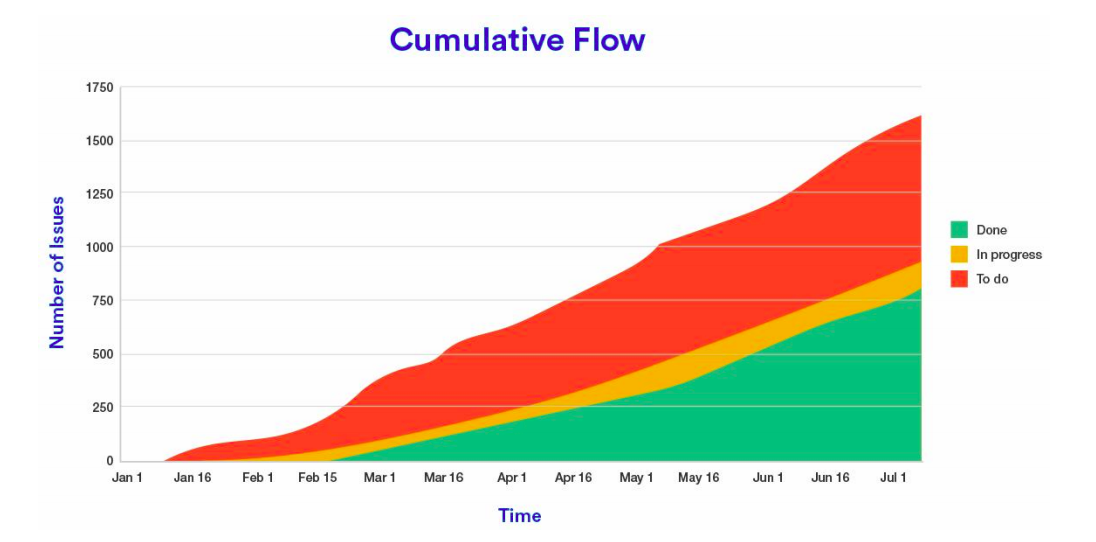
\includegraphics[width=120mm,height=80mm]{Slike/mera_napretka.png}
      \end{center}
    \end{figure}
    \item \textbf{Mera završavanja:} Umesto ostvarenih poslova se predstavljaju preostali poslovi
          u odnosu na vreme. Ima bar dve linije tj. plan i ostvarenje.
    \begin{figure}[H]
      \begin{center}
          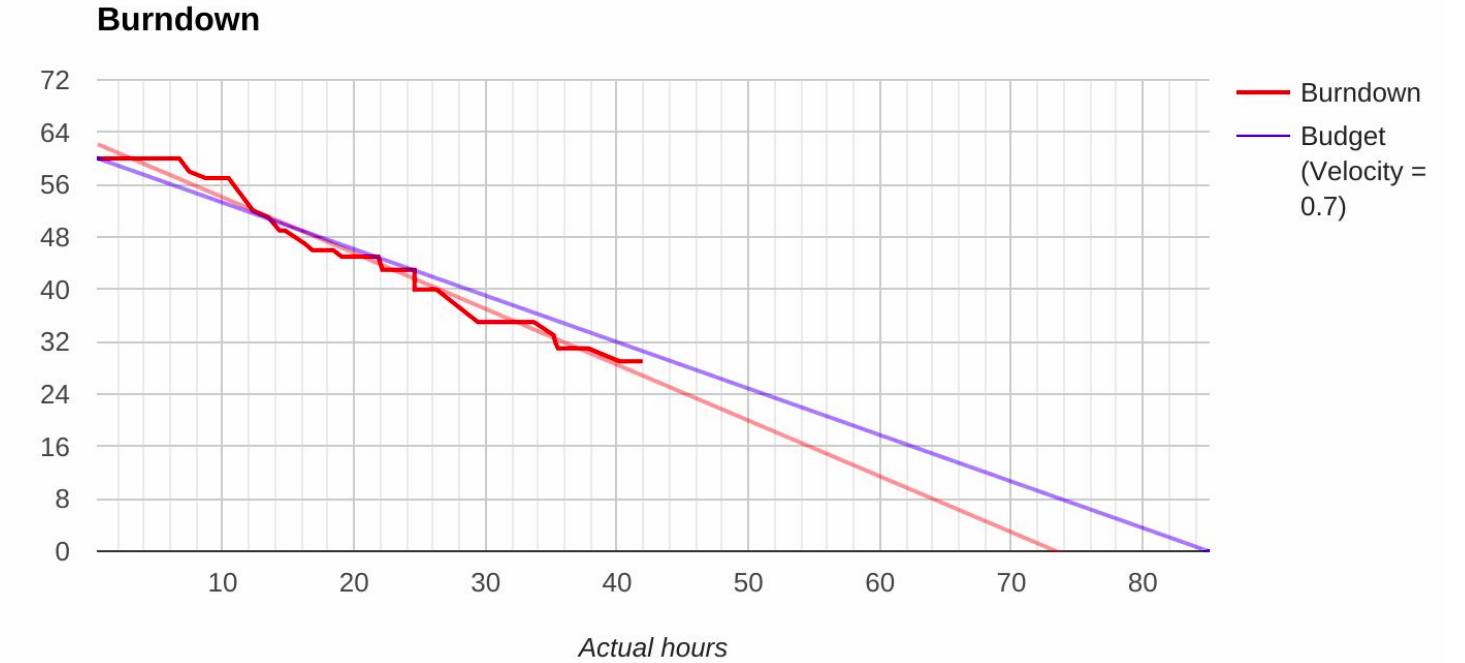
\includegraphics[width=120mm,height=80mm]{Slike/mera_dovrsavanja.png}
      \end{center}
    \end{figure}
    \item \textbf{Mera napora:} Iskazuje planirani i ostvareni broj radnih sati u odnosu na vreme.
    \begin{figure}[H]
      \begin{center}
          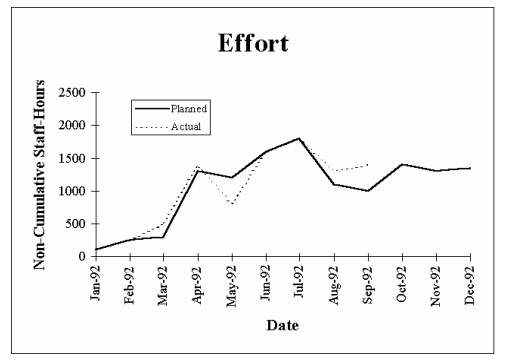
\includegraphics[width=120mm,height=80mm]{Slike/mera_napora.png}
      \end{center}
    \end{figure}
    \item \textbf{Troškovi:} Iskazuje planirani i ostvareni utrošak sredstava u odnosu na vreme. 
          Dijagram sadrži:
    \begin{itemize}
      \item projektovani ukupan budžet \textit{(BAC)};
      \item planirana vrednost \textit{(PV, planned value)} tj. planiran utrošak do tada
      \item stvaran trošak \textit{(AC, actual cost)} tj. stvaran utrošak do tada
      \item dobijena vrednost \textit{(EV, earned value)} tj. procenat obavljenog posla 
            pomnožen sa projektovanim ukupnim budžetom
    \end{itemize}
    \begin{figure}[H]
      \begin{center}
          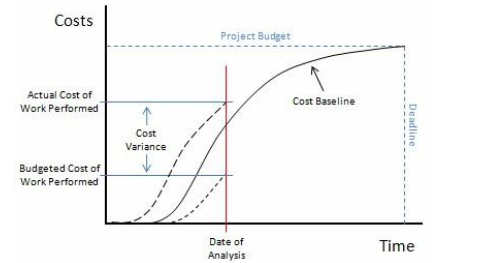
\includegraphics[width=100mm,height=60mm]{Slike/trosak.png}
      \end{center}
    \end{figure}
    \item \textbf{Problemi:} Ukazuje broj otvorenih i rešenih problema u odnosu na vreme.
          Može biti po danima ili kumulativno.
    \begin{figure}[H]
      \begin{center}
          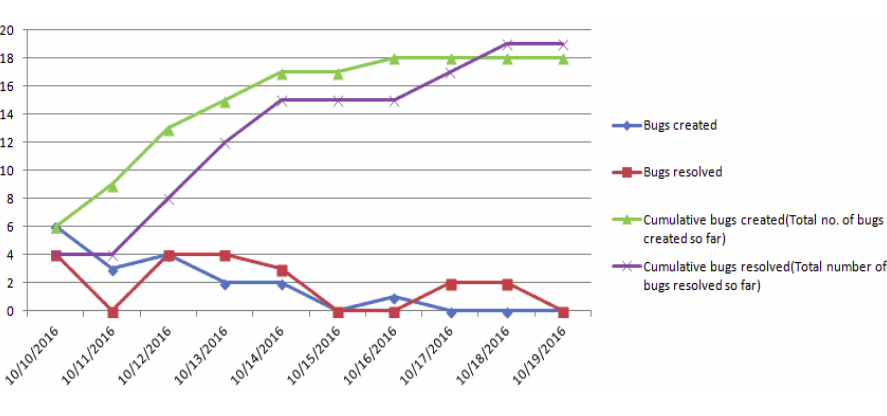
\includegraphics[width=100mm,height=60mm]{Slike/problemi.png}
      \end{center}
    \end{figure}
    \item \textbf{Stabilnost zahteva:} Iskazuje broj zahteva tokom vremena.
    \item \textbf{Stabilnost veličine:} Iskazuje veličinu softvera, obično iskazanu u 
          broju jedinica koda, tokom vremena.
  \end{itemize}
  
\section{Navesti nekoliko metrika dizajna razvoja softvera. Šta one opisuju?}
  
  Metrike dizajna softvera iskazuju različite merljive odlike softvera.\\
  
  \textbf{Neposredne mere softvera su često lako merljive veličine:}
  \begin{itemize}
    \item \textbf{Broj jedinica koda:}
      \begin{itemize}
        \item Iskazuje broj celina koda;
        \item Može da predstavlja broj:
          \begin{itemize}
            \item programskih datoteka 
            \item klasa
            \item paketa
            \item komponenti
            \item izvršnih datoteka.
          \end{itemize}
    \end{itemize}
    \item \textbf{Broj linija koda:}
      \begin{itemize}
        \item Iskazuje količinu napisanog koda;
        \item Obično obuhvata:
          \begin{itemize}
            \item Sve neprazne linije koje nisu komentari;
            \item Uključujući izvršni kod i deklaracije, definicije i druge vrste neizvršnog koda.
          \end{itemize}
      \end{itemize}
    \item \textbf{Broj funkcionalnih elemenata koda}
      \begin{itemize}
        \item Opisuje broj nekih funkcionalnih elemenata:
          \begin{itemize}
            \item Broj klasa u paketu
            \item Broj metoda u klasi
            \item Broj metoda u interfejsu paketa 
            \item ...
          \end{itemize}
      \end{itemize}
  \end{itemize}
  \textbf{Izvedene mere softvera mogu da opisuju veoma složene odlike dizajna softvera:}
  \begin{itemize}
    \item Kohezija jedinice koda;
    \item Spregnutost jedinice koda;
    \item Stabilnost jedinice koda;
    \item Apstraktnost jedinice koda.
  \end{itemize}
  
\section{Objansiti metriku stabilnost paketa.}
  Stabilnost paketa predstavlja njegovu tendenciju da se ne menja tokom vremena.
  \begin{itemize}
    \item \textbf{Spregnutost prema paketu (eng. afferent coupling):} 
          što ih je više, to će promene paketa biti teže izvodive, a time i ređe.\\
          $C_a$ = broj klasa u drugim paketima koje zavise od klasa u posmatranom paketu
    \item \textbf{Spregnutost od paketa (eng. efferent coupling):}
          što ih je više, to će njegove promene česće biti potrebne.\\
          $C_e$ = broj klasa u posmatranom paketu koje zavise od klasa u drugim paketima
    \item \textbf{Nestabilnost:} $I = \frac{C_e}{C_a + C_e}$. Ima opseg [0, 1].
  \end{itemize}
  Nije moguće da svi paketi budu stabilni. Ako bi bili, to bi značilo da je 
  čitav sistem nepromenljiv. Umesto toga želimo da neki paketi budu stabilniji, 
  a neki manje stabilni. \\
  
  \textbf{Princip odnosa zavisnosti i stabilnosti:} Zavisnost paketa bi trebalo da ide 
  od nestabilnih prema stabilnim paketima. 
  Nije dobro ako postoji zavisnosti stabilnog paketa od nekog koji je relativno 
  fleksibilan (nestabilan).\\

  Primer: Određuje se nestabilnost paketa C tj. Pc.
  \begin{figure}[H]
    \begin{center}
        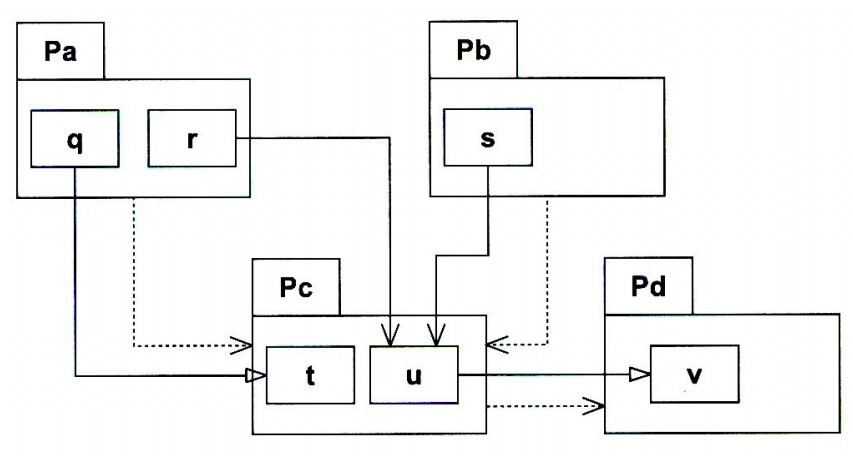
\includegraphics[width=100mm,height=60mm]{Slike/nestabilnost_primer.png}
    \end{center}
  \end{figure}
  Objašnjenje: 
  \begin{itemize}
    \item $C_a = 3$, zavisnosti klasa: $q \rightarrow t, r \rightarrow u, s \rightarrow u$
    \item $C_e = 1$, zavisnosti klasa: $u \rightarrow v$
    \item $=> I = \frac{1}{4}$
  \end{itemize}
  
\section{Objansiti metriku apstraktnost paketa.}
  Apstraktnost paketa je relativna zastupljenost apstraktnih klasa u paketu:
  \begin{itemize}
    \item \textbf{$N_a := $Broj apstraktnih klasa u paketu } 
    \item \textbf{$N_c := $broj klasa u paketu }
    \item \textbf{Apstraktnost $A$:} $A=\frac{N_a}{N_c}$ Ima opseg [0,1].
  \end{itemize}
  \textbf{Princip odnosa stabilnosti i apstraktnosti:} Paket treba da bude onoliko apstraktan 
  koliko je stabilan. Drugim rečima, manje apstraktni paketi bi trebalo da zavise od apstraktnih, 
  a ne obrnuto.
  
\section{Objasniti odnos metrika stabilnosti i apstraktnosti paketa.}
  Poželjno je da odnos apstraktnosti i stabilnosti bude što bliže glavnoj sekvenci. \\
  Udaljenost D se računa kao: \\
  \indent $D = \frac{|A+I-1|}{\sqrt{2}}$\\
  Normalizovan oblik:\\
  \indent $D = |A+I-1|$

  \begin{figure}[H]
    \begin{center}
        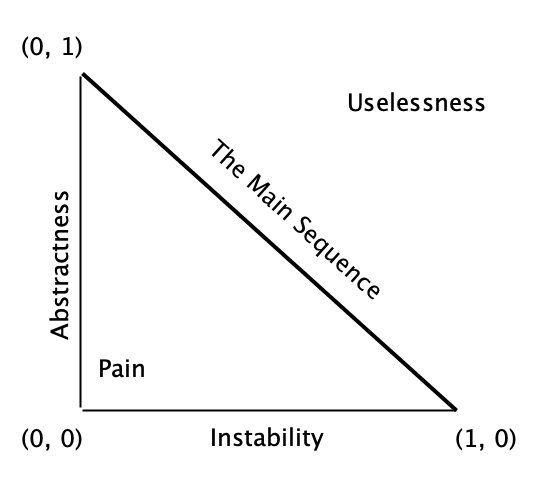
\includegraphics[width=80mm,height=60mm]{Slike/apstraktnost_i_stabilnost.jpg}
    \end{center}
  \end{figure}

\section{Objasniti metriku funkcionalna kohezija paketa.}
  Jedan način izražavanja funkcionalne kohezije paketa je u obliku količnika broja zavisnosti 
  među klasama paketa i broja paketa. Predstavlja intenzitet odnosa paketa sa sopstvenim klasama
  \begin{itemize}
    \item \textbf{$R = $Broj međusobnih zavisnosti među klasama paketa} 
    \item \textbf{$N = $Broj klasa u paketu}
    \item \textbf{$H = $Relaciona kohezija}, $H = \frac{R+1}{N}$
  \end{itemize}
  Alternativa je da se svaka zavisnost dveju klasa predstavi brojem metoda koji je ostvaruju.
  
\section{Šta su sistemi za kontrolu verzija? Objasniti.}
  Sistem za kontrolu verzija je softver za upravljanje izmenama u programskom kodu, 
  dokumentima i drugim vrstama fajlova. Obično se razmatra u kontekstu projekata razvoja 
  softvera, ali može imati i druge namene. Postoji veliki broj sistema za kontrolu verzija:
  \begin{itemize}
    \item CVS
    \item SVN (Subversion)
    \item Git
    \item Bazaar
    \item ...
  \end{itemize}
\section{Objasniti arhitekturu i navesti osnovne operacije pri radu sa sistemima za kontrolu verzija.}
  Sistem za kontrolu verzija (SKV) obično ima arhitekturu klijent-server. 
  Server je instanca sistema za kontrolu verzija, a klijent je korisnik SKV.
  Neki sistemi imaju distribuiranu arhitekturu:
  \begin{itemize}
    \item decentralizovani
    \item omogućavaju podnošenje i bez povezivanja sa serverom
    \item odlaganje razrešavanja i spajanja
  \end{itemize}
  SKV (bilo da je centralizovan ili distribuiran) sadrži spremište. 
  Spremište je mesto na kome se čuvaju različite verzije projekta. 
  Obično se implementira pomoću odgovarajuće baze podataka.
  
  \textbf{Koncept upotrebe:} Prvi korak je pravljenje radne kopije:
  \begin{itemize}
    \item Radna kopija (eng. working set, working copy) je lokalna kopija verzije na klijentu, 
          koja se menja tokom rada;
    \item Osim fajlova projekata sadrži i metapodatke o verzijama fajlova;
    \item Postupak pravljenja radne kopije se naziva preuzimanje (eng. checkout);
    \item Radna kopija ne mora uvek da se pravi samo na osnovu osnovne linije.
  \end{itemize}
  Po potrebi se radna kopija može ažurirati (eng. update, sync) preuzimanjem aktuelne verzije 
  iz spremišta. Nakon menjanja fajlova radne kopije, izmenjena verzija se podnosi 
  (eng. commit, checkin, install, record) tj. postavlja se u spremište kao nova aktuelna verzija.\\
  
  \textbf{Uvoz i izvoz:} Nakon pravljenja novog projekta u spremištu, obično se projekat inicijalno 
  popunjava uvozom (eng. import) odgovarajuće lokalne kopije.\\
  \indent Po potrebi se verzija može izvoziti (eng. export), pri čemu se pravi nova lokalna kopija, 
  nalik na radnu kopiju, ali koja ne sadrži metapodatke o preuzimanju i spremištu.\\
  
  \textbf{Osnovna linija:} Sekvenca verzija koje se uzastopno menjaju naziva se glavna linija. 
  Usled mogućnosti grananja, može postojati više glavnih linija. Osnovna glavna linija se naziva 
  osnovna linija (eng. trunk, main, baseline). Poslednje podnošenje osnovne linije se naziva 
  glava (eng. head).\\
  
  \textbf{Izmene:} Svakim podnošenjem se prave nove verzije pojedinačnih menjanih fajlova i 
  nova verzija projekta. Izmene se prave pravljenjem novih grana. Poseban vid izmena je tzv. 
  promocija (eng. promote) - kopiranje verzije fajla koja nije kontrolisana u spremište 
  (ili radnu kopiju).
   
\section{Šta je spremište? Šta sadrži? Kako je organizovano?}
  SKV (bilo da je centralizovan ili distribuiran) sadrži spremište. 
  Spremište je mesto na kome se čuvaju različite verzije projekta. 
  Obično se implementira pomoću odgovarajuće baze podataka.

\section{Šta je radna kopija u kontekstu upotrebe sistema za kontrolu verzija?}
  \begin{itemize}
    \item Radna kopija (eng. working set, working copy) je lokalna kopija verzije na klijentu, 
          koja se menja tokom rada;
    \item Osim fajlova projekata sadrži i metapodatke o verzijama fajlova;
    \item Postupak pravljenja radne kopije se naziva preuzimanje (eng. checkout);
    \item Radna kopija ne mora uvek da se pravi samo na osnovu osnovne linije.
  \end{itemize}
\section{Objasniti pojam oznake u kontekstu upotrebe sistema za kontrolu verzija.}
  Često je pojedine verzije potrebno posebno označiti:
  \begin{itemize}
    \item Primer: verzija koja se javno publikuje;
    \item Ali i verzija koja predstavlja neki interno značajan trenutak.
  \end{itemize}
  Označena verzija (ili kraće samo oznaka) (eng. tag, label) je verzija koja je posebno 
  označena radi kasnijeg referisanja:
  \begin{itemize}
    \item Verzija se označava davanjem odgovarajućeg imena;
    \item U zavisnosti od sistema postoji određena sloboda u određivanju naziva oznake.
  \end{itemize}
  
\section{Objasniti grananje u kontekstu upotrebe sistema za kontrolu verzija.}
  Često je potrebno istovremeno razvijavati više različitih verzija koda:
  \begin{itemize}
    \item Primer: i nakon objavljivanja nove verzije potrebno je razvijati popravke za staru;
    \item Razvijanje novih funkcija za koje se ne zna kada će biti uvrstene u osnovnu liniju.
  \end{itemize}
  Verzija koja se razvija nezavisno od glavne linije razvoja naziva se grana (eng. branch). 
  Svaka grana ima svoju glavnu liniju, kao što čitav projekat ima svoju osnovnu liniju. 
  Fajlovi i direktorijumi se mogu deliti između grana - izmene deljenih fajlova se takode dele u 
  svim granama. Grane se u nekim slučajevima spajaju nazad u stablu. To se naziva povratno 
  integrisanje (eng. reverse integration). Npr. razvijanje komponente za koju nije unapred 
  poznato kada će biti uključena u osnovnu liniju.

\section{Šta su konflikti i kako se rešavaju u kontekstu upotrebe sistema za kontrolu verzija?}
  \noindent Često se dešava da se neki fajl menja od strane više klijenata ,,istovremeno``:
  \begin{itemize}
    \item Ko prvi podnese izmenjen fajl, imaće jednostavniji posao;
    \item Onaj ko pokuša podnošenje kao drugi, biće obavešten da je fajl u međuvremenu 
          menjan i da je potrebno da preduzme spajanje verzija.
  \end{itemize}
  Konflikti se, pored opisanog slučaja, dešavaju i kada se:
  \begin{itemize}
    \item Neka grana spaja sa stablom ili sa drugom granom;
    \item U jednoj grani se ispravi neki problem koji je postojao i pre grananja, 
          pa je potrbno ispravke preneti i u ostale grane.
  \end{itemize}
\section{Šta je spajanje verzija u kontekstu upotrebe sistema za kontrolu verzija?}
  Spajanje verzija (eng. merge, integration) je operacija spajanja dva skupa izmena fajla ili 
  skupa fajlova. Primenjuje se kada je potrebno rešiti konflikte. Sastoji se od skupa pojedinačnih 
  razrešavanja (eng. resolve) problema. Razrešavanje je manuelna intervencija radi rešavanja 
  sukobljenih izmena na istom dokumentu.
  
\section{Objasniti primer strategije označavanja verzija.}
  Određivanje strategije označavanja verzija je sastavni deo upravljanja razvojnim projektom. 
  Uobičajeno cetvorodelno označavanje verzije:\\
  \indent $<glavna verzija>.<podverzija>[.<popravka>[.<revizija>]]$\\
  \textbf{Glavna verzija:}
  \begin{itemize}
    \item Menja se kada su uvedene značajne izmene u odnosu na prethodnu verziju softvera;
    \item ,,Značajne izmene`` može da ima različita značenja;
    \item Dodate su suštinski nove funkcije;
    \item Kod je pisan u potpunosti iznova;
    \item Softver se prodaje kao poseban proizvod.
  \end{itemize}
  \textbf{Podverzija:}
  \begin{itemize}
    \item Menja se kada su uvedene izmene koje nisu samo popravke uočenih nedostataka, 
          ali ne zavređuju novu glavnu verziju;
    \item Dodate su neke nove funkcije;
    \item Menjane su neke postojeće funkcije.
  \end{itemize}
  \textbf{Popravka:}
  \begin{itemize}
    \item Podrazumeva da nisu uvedene izmene u funkcionalnosti softvera već samo ispravke 
          uočenih nedostataka;
    \item Nekad su kao sastavni deo ispravki obezbeđene i manje izmene ili novine.
  \end{itemize}
  \textbf{Revizija:}
  \begin{itemize}
    \item Broj koji označava reviziju popravke;
    \item Obično predstavlja smao internu oznaku za izmene koda ili dokumentacije koje 
          imaju sasvim ograničen značaj.
  \end{itemize}
  
  Često se razdvajaju javni i interni brojevi verzija. Javne verzije se obično sastoje od dva dela, 
  a popravke se ili dodaju kao treći broj ili se označavaju opisno:
  \begin{itemize}
    \item DB2 v9.1 
    \item xpack 3
    \item Firefox 3.6.3
  \end{itemize}
  Brojevi popravke i revizija su često internog karaktera i koriste se samo u okviru razvojnog tima.\\
  \textbf{Dodatne oznake:} Da bi bio jasan kontekst neke verzije, često se broju dodaju opisni 
  elementi. Primer:
  \begin{itemize}
    \item 3.1a - alfa verzija, interna pregledna verzija;
    \item 3.1b - beta verzija, interna verzija koja može koristiti radi upoznavanja softvera 
          ali nije jos dovršena;
    \item 3.1rc1 - kandidat za objavljivanje, predstoje samo popravke poznatih i 
          kasnije uočenih nedostataka i eventualno dodavanje nekih manjih funkcionalnosti 
          za koje se naknadno ustanovi da su neophodne;
    \item 3.1rc2 - kandidat za objavljivanje, predstoje samo popravke poznatih i 
          kasnije uošenih nedostataka.
  \end{itemize}
  \textbf{Postupak numerisanja:} 
  \begin{itemize}
    \item Obično se pre prvog publikovanja softver vodi sa glavnim brojem 
          verzije ,,0``. Sve verzije koje prethodne verziji ,,1`` su ,,nezvanične``. 
    \item Ne postoji koncenzus oko 
          toga kako se interno numerisu interne razvojne verzije koje prethode novoj 
          glavnoj verziji.
  \end{itemize}
  \textbf{Numerisanje razvojnih verzija:}
  \begin{itemize}
    \item v1:
        \begin{itemize}
          \item nova glavna verzija ima sve ostale brojeve verzije (osim glavnog) jednake ,,0``
          \item 2.0.0
          \item tada je problem numerisanja internih verzija
          \item obično razvoj verzija 2 u takvim uslovima počinje od npr. 1.9.0.0
        \end{itemize}
    \item v2:
        \begin{itemize}
          \item prva interna verzija koda nove glavne verzije odmah dobija svoj glavni broj
          \item tada se publikovanje odvija sa nekim drugim brojem, na primer 2.0.7
        \end{itemize}
    \item v3: broju popravke se daju posebna znacenja, na primer:
        \begin{itemize}
          \item 2.0.0.x - alfa verzija
          \item 2.0.1.x - beta verzija
          \item 2.0.2.x - kandidat za objavljivanje
          \item 2.0.3.x - kandidat za objavljivanje 2
          \item 2.0.4.x - objavljena verzija
        \end{itemize}
    \item v4:
        \begin{itemize}
          \item Potpuno se razdvajaju interni brojevi verzija od javnih
          \item Interna verzija 2.0.12.5 se proglašava za javnu verziju 2.0.0
        \end{itemize}
  \end{itemize}
  \textbf{Numerisanje razvojnih verzija:} Svaki od brojeva počinje od 0 i povećava se. Primer: 
  verzija 3.2.0 je posle verzije 3.1.6. Za sve brojeve, osim poslednjeg, uobičajeno je da se 
  vraćaju na 0 kada se prethodni broj promeni:
  \begin{itemize}
    \item Posle 3.1.6 ide 3.2.0;
    \item Tako se omogućava da se i posle objavljivanja nove verzije (podverzije) i dalje 
          obezbeđuju popravke prethodnih verzija (posle 3.2.0 može da se objavi 3.1.7).
  \end{itemize}
  \textbf{Poslednji broj može da ima različito značenje:}
  \begin{itemize}
    \item Revizija u okviru popravke - vraća se na nulu nakon promene broja popravke;
    \item Redni broj punog građenja sistema:
          \begin{itemize}
            \item Nikada se ne vraća na 0;
            \item Tada je samo ovaj broj dovoljan za interno označavanje verzije;
            \item Obično se taj broj koristi samo za interne svrhe;
            \item Samo prva 2 ili 3 se koriste za javno označavanje.          
          \end{itemize}
    \item Primer:
      \begin{itemize}
        \item 2.0.0.782 
        \item 2.0.0.791.a 
        \item 2.0.0.842.b 
        \item 2.0.0.864.rc1 
        \item 2.0.0.872.rc2
        \item 2.0.0.875.public 
        \item javno objavljena verzija 2.0
      \end{itemize}
  \end{itemize}
  
\section{Šta su sistemi za praćenje zadataka i bagova? Objasniti namenu i osnovne elemente.}
  Sistemi za praćenje bagova predstavljaju alate za upravljanje evidencijom i komunikacijom u 
  vezi sa uočenim neispravnostima. Predstavljaju poseban slučaj opštijih sistema za praćenje zadatka. 
  Nazivaju se i sistemi za praćenje poslova. Engleski termini: 
  \begin{itemize}
    \item bug tracking system
    \item issue tracking system
    \item ticket system
    \item \dots
  \end{itemize}
  
\section{Navesti i ukratko objasniti osnovne koncepte sistema Red-mine.}
  Savremeni sistemi za praćenje poslova su fleksibilni:
  \begin{itemize}
    \item Podržavaju više vrsta kartica (npr. bagovi, zadaci, nadogradnje, diskusije i sl.);
    \item Za svaku vrstu se mogu definisati različita stanja i načini prolazaka kroz stanja;
    \item Različite grupe korisnika imaju različita prava, u zavisnosti od stanja kartice;
    \item Automatsko slanje obaveštenja elektronskom poštom;
    \item Dokumentacija;
    \item Programski kod;
    \item ...
  \end{itemize}
  
\section{Objasniti ulogu stanja kartica i način njihovog menjanja (na primeru sistema Redmine).}
  Kartica (ili stavka, eng issue, ticket) je jedan evidentiran bag / problem / posao / zadatak
  \begin{itemize}
      \item Kartica predstavlja centralni objekat svakog sistema za praćenje zadatka;
      \item Kartica može imati različita stanja koja opisuju koje se aktivnosti očekuju 
            u odnosu na zadatak;
      \item Obično joj se može dodeljivati kategorija, prioritet, detaljan opis.
  \end{itemize}
\section{Šta čini dokumentaciju softvera?}
  Dokumentacija softvera je tekst i/ili ilustracija koja prati računarski softver. 
  Ona objašnjava kako se koristi softver ili kako on radi. Može da ima različito značenje za 
  različite tipove korisnika.
  Obično sadrži:
  \begin{itemize}
    \item Opis atributa, mogućnosti ili karakteristike softvera.
    \item Opis namene - šta softver radi (ili bi trebalo da radi).
    \item Arhitekturu/dizajn softvera - opis samog softvera. Uključuje odnose 
          softverskih komponenti sa okruženjem.
    \item Tehničku dokumentacija - sastoji se od koda, algoritama, interfejsa, i 
          aplikacionog programskog interfejsa.
    \item Korisničku dokumentaciju - uputstva za krajne korisnike, administratore sistema i 
          stručno osoblje.
    \item Marketing - kako da se reklamira i prodaje proizvod i analizu zahteva tržišta.
  \end{itemize}
\section{Kome je i zašto potrebna dokumentacija?}
  Svima, ali svakome na drugi način i u drugačijem obliku\\
  \textbf{Naručiocu posla:}
  \begin{itemize}
    \item Da zna šta je naručio;
    \item Da bude siguran da izvođači znaju šta je naručio;
    \item Da misli da je dobio šta je tražio.
  \end{itemize}
  \textbf{Rukovodiocima projekta:}
  \begin{itemize}
    \item Da vide šta su zahtevi;
    \item Da vide šta je urađeno.
  \end{itemize}
  \textbf{Projektantima:}
  \begin{itemize}
    \item Da znaju šta je potrebno da naprave;
    \item Da zapišu implementatorima kako zamišljaju da to naprave;
    \item Da misle da je implementirano ono što su isprojektovali i kako su isprojektovali.
  \end{itemize}
  \textbf{Implementatorima:}
  \begin{itemize}
    \item Da znaju šta je potrebno da naprave;
    \item Da znaju kako je potrebno da to naprave;
    \item Da izveste rukovodioce o tome kako veruju da su to napravili;
    \item Da objasne budućim korisnicima programskog koda šta je šta i čemu služi;
    \item Da objasne korisnicima softvera šta softver radi i kako se koristi.
  \end{itemize}
  \textbf{Korisnicima:} 
  \begin{itemize}
    \item Da vide čemu softver služi i kako se upotrebljava.
  \end{itemize}
  
\section{Navesti i ukratko objasniti osnovne opravdane i 
         neopravdane motive za pravljenje dokumentacije.}
  \noindent \textbf{Zato što to traži klijent:}
  \begin{itemize}
    \item U pitanju je poslovna odluka (opravdano): Klijent obično ne ume da proceni potreban obim, 
          kao ni pravi trenutak za pisanje dokumentacije (neopravdano).
    \item Iz ugla razvojnog tima je to legitiman razlog, ali je istovremeno i frustrirajuće (opravdano).
    \item Često proizvodi nepotrebne troškove, bez značajnih pozitivnih posledica ako nije 
          praktično neophodna u trenutku kada se traži (neopravdano).
  \end{itemize}
  \textbf{Da bi se formalizovale specifikacije (opravdano):}
  \begin{itemize}
    \item \underline{Formalizovanje interfejsa za upotrebu komponenti:} 
          Važno za sve koji će razvijati i koristiti komponentu.
    \item \underline{Precizno objavljivanje ponašanja komponenti:}
          Važno za sve koji će razvijati i koristiti komponentu.
    \item \underline{Konceptualan i implementacioni model komponente:} 
          Važno svim učesnicima u njenom razvoju.
  \end{itemize}
  \textbf{Da bi se podržala komunikacija sa udaljenim timovima (opravdano):}
  \begin{itemize}
    \item Nisu uvek svi članovi tima na istoj lokaciji;
    \item Dokumentacija je kao vid statičke komunikacije pogodna za informisanje 
          dislociranih članova tima. 
    \item Posebno važno u slučaju otvorenih projekata, autsorsinga i slično;
  \end{itemize}
  \textbf{Da bi se definisali ciljevi rada za neku drugu grupu:}
  \begin{itemize}
    \item U nekim slučajevima može da bude dobro (opravdano): 
          \begin{itemize}
            \item Ako je u pitanju specifikacija onoga što se 
                  pravi u tekućem razvojnom ciklusu 
            \item Ako samo ukratko i konceptualno ukazuje na dalje planove;
          \end{itemize}
    \item Ali često nije dobro (neopravdano):
      \begin{itemize}
        \item Ako je dokumentacija nepotrebno detaljna i obimna;
        \item Ako opisuje zadatke i ponašanje koji nisu deo tekućeg razvojnog ciklusa.
      \end{itemize}
    \item Usmena komunikacija je obično efikasnija.
  \end{itemize}
  \textbf{Da bi se podstaklo širenje i memorisanje informacija u timu (opravdano):} 
    \begin{itemize}
      \item informacije o urađenom i planiranom su važne za razvoj, održavanje i upotrebu.
    \end{itemize}
  \textbf{Radi praćenja razvoja:}
  \begin{itemize}
    \item Dokumentacija omogućava uvid u dostignuća razvoja (za to nije potrebna obimna i 
          precizna dokumentacija) (opravdano);
    \item Klijenti često imaju stav da je dokumentacija pokazatelj uspešnosti razvoja, što  je potpuno 
          pogrešno. Dokumentacija se može napisati i o nečemu što nije čak ni dovoljno detaljno 
          zamišljeno, a kamoli napravljeno (neopravdano).
  \end{itemize}
  \textbf{Da bi se nešto temeljno razmotrilo (opravdano):}
  \begin{itemize}
    \item Pisanje dokumentacije je dobar vid proveravanja pretpostavki.
    \item Pri pisanju dokumentacije se podstiče kritičko razmatranje.
    \item Ovaj motiv često podstiče specifične vidove dokumentacije, čija važnost rapidno 
          opada sa protokom vremena.
  \end{itemize}
  \textbf{Po inerciji (neopravdano):}
  \begin{itemize}
    \item Posledica navike klijenta: Klijent ne zna za drugačiju praksu, ali to ne znači ni da 
          je ona dobra, ni da je loša, ali navika nije opravdanje.
    \item Zato što razvojni proces tako propisuje. Nijedan proces nije dovoljno dobar i pouzdan 
          da se slepo sledi.
  \end{itemize}
  \textbf{Kao vid obezbeđenja klijenta (neopravdano):}
  \begin{itemize}
    \item Ako razvijalac nije dovoljno dobar, onda klijent može predati projekat i dokumentaciju 
          drugom izvođacu, da bi nastavio posao (opravdano);
    \item Ali ako razvijalac nije dovoljno dobar, onda nije dobra ni dokumentacija;
    \item Informacije razmenjene u ovom obliku često su dezinformacije o pogrešnim planovima;
    \item Čak i kada je dokumentacija dobra, ona opisuje kako je nešto isplanirao jedan tim, 
          a drugi može da ima drugacije iskustvo, pristupe problemu i praksu.
  \end{itemize}
  
\section{Objasniti ulogu dokumentacije kao vida specifikacije zahteva projekta.}
  Pogledati prethodno pitanje.
  
\section{Objasniti ulogu dokumentacije kao sredstva za komunikaciju.}
  Pogledati prethodno pitanje.
  
\section{Objasniti ulogu dokumentacije u razmatranju nedoumica u projektu.}
  Pogledati prethodno pitanje.
  
\section{Objasniti podelu dokumentacije po nameni.}
  \noindent Prema nameni se razlikuju:
  \begin{itemize}
      \item \textbf{Korisnička dokumentacija:} Namenjena je krajnjem korisniku softvera. 
            Objašnjava sve aspekte primene softvera.
      \item \textbf{Tehnička dokumentacija:} Namenjena je svim (sadašnjim i budućim) učesnicima u 
            razvoju ili održavanju softvera. Namenjena je i tehničkim licima koja moraju da pružaju 
            podršku korisnicima.
  \end{itemize}
  Dokumentacija se odnosi na ceo softverski projekat:
  \begin{itemize}
      \item Ne samo na gotov program;
      \item Ne samo na postavljen zadatak;
      \item Vec na sve segmente posla, od prve zamisli o softveru do gotovog softvera.
  \end{itemize}

\section{Šta obuhvata korisnička dokumentacija softvera?}
  \begin{enumerate}
    \item \textbf{Opis čitavog sistema:} Uopšteni opis funkcija koje sistem pruža;
    \item \textbf{Uputstvo za instalaciju:} Objašnjava kako se sistem priprema za rad, 
          kako se prilagođava specifičnom okruženju, potrebama korisnika ili konkretnom 
          računarskom sistemu;
    \item \textbf{Vodič za početnike:} Pruža pojednostavljena objašnjenja kako započeti upotrebu 
          sistema, obično u obliku tutorijala;
    \item \textbf{Referentni priručnik:} Detaljan opis svih karakteristika i mogućnosti sistema 
          i načina njihove upotrebe;
    \item \textbf{Prilog o dopunama:} Opis izdanja pregledni izveštaj o svim izmenama i dopunama 
          novog izdanja softvera;
    \item \textbf{Skraćeni referentni pregled:} Pomoćni priručnik za brzo podsećanje;
    \item \textbf{Upuststvo za administraciju:} Tehnički priručnik sa detaljnim objašnjenjima o 
          mogućim naprednim prilagođavanjima specifičnim okolnostima i sa detaljnim opisom problema.
  \end{enumerate}
  
\section{Šta obuhvata tehnička (sistemska) dokumentacija softvera?}
  \begin{enumerate}
    \item \textbf{Vizija:} Objašnjava ciljeve sistema;
    \item \textbf{Specifikacija i analiza zahteva:} Pruža detaljan opis zahteva ugovorenih 
          između zainteresovanih strana (naručioci, klijenti, korisnici, projektanti, izvođači . . . )
    \item \textbf{Specifikacija ili projekat:} Detaljni opisi svih aspekata implementacije:
      \begin{itemize}
        \item Kako se sistem deli na celine;
        \item Kako se implementiraju pojedinačni zahtevi ili celine;
        \item Koju ulogu ima koja komponenta sistema.
      \end{itemize}
  \item \textbf{Opis implementacije - Detaljni opisi:}
    \begin{itemize}
      \item Kako se pojedini elementi sistema modeliraju na konkretnim programskim jezicima;
      \item Opisi značajnijih algoritama;
      \item Specifikacije komunikacije.
    \end{itemize}
  \item \textbf{Plan testiranja softvera:} Opis protokola testiranja softvera (testovi jedinica koda 
        i sve ostale vrste razvojnih testova);
  \item \textbf{Rečnik podataka:} Sadrži rečnik termina i posebno opis osnovnih vrsta podataka 
        koji se koriste u sistemu.
  \item \dots
  \end{enumerate}
\section{Kakav je odnos agilnog razvoja softvera prema pisanju dokumentacije? 
         Koji vidovi dokumentacije se podstiču a koji ne?}
  Agilne metodologije podstiču specifičan pristup pravljenju i održavanju dokumentacije.\\
  \textbf{Motivacija:} 
  \begin{itemize}
    \item \textbf{Razvojna dokumentacija je često neažurna};
    \item \textbf{Velika količina dokumentacije nije korisna:} Ili bude izmenjena pre upotrebe 
          ili postane neažurna;
    \item \textbf{Dokumentacija nije cilj nego sredstvo za ostvarenje komunikacije};
    \item \textbf{Cena održavanja dokumentacije je visoka};
  \end{itemize}

  \textbf{Specifikacije:} U agilnom razvoju dokumentacija je u obliku korisničkih celina 
  (sasvim površne). Korisničke celine: Samo okvirni opis, bez pojedinosti, ukazuje se na sadržaj i 
  obim.\\

  \textbf{Modeli:} početna faza implementacije korisničkih celina je pravljenje modela. 
  Modeli su deo razvojne dokumentacije. Na osnovu njih može da se pravi i formalna dokumentacija, 
  ali najčešće prestaje da bude ažurna već tokom razvoja. Modeli se prave u različitim fazama 
  implementacije. Predstavljaju sredstvo za razmatranje i razmenu informacija o konceptualnom rešenju. 
  Neophodan su deo razvojne dokumentacije ali najčešće postaje neažuran već tokom razvoja, ili 
  kasnije, tokom održavanja. Neažurna dokumentacija je dezinformacija. Mogu da prerastu u trajnu 
  dokumentaciju ako je model stabilan, ako je značajan za buduće faze razvoja, ako klijent želi da 
  investira.\\

  \textbf{Dokumenti:} Ozvaničeni modeli, opisi ponašanja ili programskog koda. Prave se relativno 
  retko, zato što ih je skupo održavati, osim ako su potrebni za dalji rad (uključujući održavanje). 
  Važno je da imaju oznake ažurnosti.\\

  \textbf{Programski kod:} Dobar programski kod je najbolji vid dokumentacije. 
  Komentari omogućuju automatsko pravljenje ažurne dokumentacije.
  Programski kod mora da se pravi, štaviše, to je cilj. Uvek ažurno predstavlja aktuelno 
  stanje razvoja. Važno je da ima dobru strukturu, radi lakšeg razumevanja i radi lakšeg održavanja 
  (refaktorisanje). Testovi jedinica koda u agilnom razvoju su u obliku korisničkih 
  celina (sasvim površne).
  
\section{Šta su alati za unutrašnje dokumentovanje programskog koda? Zašto su potrebni i po čemu 
         se suštinski razlikuju od održavanja spoljašnje dokumentacije?}
  Unutrašnja dokumentacija objašnjava kako kod funkcioniše (primer: komentari u kodu), a
  spoljašnja dokumentacija objašnjava kako se softver koristi.\\

  Alati za unutrašnje dokumentovanje programskog koda služe za automatsko generisanje
  skeleta dokumentacije, što značajno olakšava posao.
\section{Šta je Doxygen? Šta omogućava? Navesti primere anotacije koda.}
  \begin{itemize}
    \item Veoma široko usvojen alat za dokumentovanje programskog koda.
    \item Praktično standard za programske jezike: C++, C, Objective	C, C\#, PHP, Java, Python, IDL
    \item Pravi dokumentaciju u HTML-u za onlajn pregledanje.
    \item Pravi dokumentaciju u LATEX, RTF, PostScript, PDF ili Unix man formatu.
    \item Dokumentacija se pravi automatski na osnovu anotiranih izvornih fajlova. 
    \item Može da se konfiguriše da napravi dokumentaciju na osnovu strukture koda čak i iz 
          izvornih fajlova koji nisu posebno anotirani. 
    \item Automatsko ilustrovanje dokumentacije 
          grafovima zavisnosti, dijagramima nasleđivanja i dijagramima saradnje.
    \item Može da se koristi i za pravljenje obične dokumentacije.
    \item Anotacija programskog koda se vrši navođenjem specifičnih oblika komentara, 
          koje Doxygen izdvaja i od njih pravi dokumentaciju.
  \end{itemize}

  \noindent \textbf{Primeri anotacija:}\cite{doxygen_commentblocks}
  \begin{itemize}
    \item Javadoc stil:
    \begin{lstlisting}
      /**
       * ... text ...
       */\end{lstlisting}
    \item QT stil:
      \begin{lstlisting}
        /*!
         * ... text ...
         */\end{lstlisting}
    \item C++ stil (1):
    \begin{lstlisting}
      /// 
      /// ... text ...
      /// \end{lstlisting}
    \item C++ stil (2):
    \begin{lstlisting}
      //! 
      //! ... text ...
      //! \end{lstlisting}
    \item Uokvireni stil (1):
    \begin{lstlisting}
      /********************************************//**
      *  ... text
      ***********************************************/\end{lstlisting}
    \item Uokvireni stil (2):
    \begin{lstlisting}
      /////////////////////////////////////////////////
      /// ... text ...
      /////////////////////////////////////////////////\end{lstlisting}
    \item Širi opis (preko komande \textbackslash brief)
    \begin{lstlisting}
    /*! \brief Brief description.
     *         Brief description continued.
     *
     *  Detailed description starts here.
    */\end{lstlisting}
    \item Dokumentacija članova(više opcija):
    \begin{lstlisting}
    int var; /*!< Detailed description after the member */
    
    int var; /**< Detailed description after the member */
  
    int var; //!< Detailed description after the member
             //!< 
            
    int var; ///< Detailed description after the member
             ///< 
            
    int var; //!< Brief description after the member 
  
    int var; ///< Brief description after the member\end{lstlisting}
    \item Dokumentacija parametara funkcije:
    \begin{itemize}
      \item @param za informaciju o parametrima
      \item {[in]}, [out], [in,out] za smer parametara
    \end{itemize}
    \begin{lstlisting}
    void foo(int v /**< [in] docs for input parameter v. */);\end{lstlisting}
    
  \end{itemize}
\section{Šta je optimizacija softvera?}
  Optimizacija softvera je proces menjanja strukture i implementacije programa u cilju postizanja 
  manjeg zauzeća resursa:
  \begin{itemize}
    \item procesorskog vremena
    \item radne memorije
    \item prostora u trajnom skladištu
    \item i drugo
  \end{itemize}
  Veoma često ušteda na jednom resursu podiže opterećenje drugog.\
  Optimizacija softvera je raspoređivanje opterećenja po resursima u skladu sa potrebama.

\section{Koje su informacije neophodne za uspešnu optimizaciju?}
  \begin{itemize} 
    \item Razumevanje problema i rešenja:
      \begin{itemize}
        \item zadatak
        \item algoritmi
        \item implementacija 
      \end{itemize}
    \item Razumevanje ograničenja:
      \begin{itemize}
        \item poslovni zahtevi
        \item arhitektura računara
        \item arhitektura procesora 
      \end{itemize}
    \item Poznavanje alata:
      \begin{itemize}
        \item programski jezik
        \item asembler i mašinski jezik
        \item alati za merenje performansi
      \end{itemize}
  \end{itemize}
  
\section{Objasniti ,,optimizaciju unapred``. Dobre i loše strane?}
  Kontinualno staranje o performansama. Ako u toku razvoja znamo koje delove je potrebno optimizovati.
  Neophodno je pažljivo struktuiranje koda sa definisanjem ciljnih performansi svake od komponenti.
  Potencijalni problemi:
  \begin{itemize}
    \item Da li smo sigurni da znamo koji su to delovi?
    \item Da li smo sigurni koje su kritične granice performansi?
    \item Da li smo sigurni da taj deo koda neće biti menjan ili izbačen?
  \end{itemize}
\section{Objasniti ,,optimizaciju unazad``. Dobre i loše strane?}
  Nakon izvršenog razvoja mere se performanse, sagledavaju se problemi i planiraju optimizacije.
  Potencijalni problemi:
  \begin{itemize}
    \item Da li upotrebljen algoritam uopšte može da se optimizuje?
    \item Da li implementirana arhitektura softvera može da se optimizuje?
  \end{itemize}
\section{Kakva je suštinska razlika između optimizacija unapred i unazad? 
         Kada je bolje primeniti koju od njih?}
  Najčešće je mnogo bolje da se optimizuje unazad.
  Optimizacija unapred značajno otežava održavanje softvera.
  Dobar dizajn softvera omogućava relativno lako održavanje, pa čak i zamenjivanje algoritama ili 
  nekih delova arhitekture. Na taj način se omogućava zadržavanje obe verzije koda (optimizovane i 
  neoptimizovane), čime se omogućava lakša lokalizacija eventualnih bagova.

\section{Koji osnovni problem proizvodi primena optimizacije u agilnom razvoju softvera? 
         Kako se prevazilazi?}
  
  \textbf{Prevremena optimizacija:} Optimizacija preduzeta pre nego što znamo šta je i koliko je
  potrebno da se optimizuje. Sukobljava se sa principom agilnog razvoja ,,neće biti potrebno``.\\
  \indent \textbf{,,Optimizuj kasnije``:} je primena principa ,,neće biti potrebno`` na problem 
  optimizacije. ,,Neće biti potrebno``: "Implementiraj tek onda kada je potrebno, 
  a ne kada predvidas da će biti potrebno!"
   
\section{Kako se dele tehnike optimizacije? Navesti nekoliko primera.}
  Dele se na: 
  \begin{itemize}
    \item \textbf{Opšte tehnike:} Tehnike koje mogu da se primene na sve ili bar veći broj 
          različitih programskih jezika ili problema i na 
    \item \textbf{Specifične tehnike:} tehnike koje se mogu primeniti na manji broj programskih jezika.
  \end{itemize}
\section{Navesti bar 7 opštih tehnika optimizacije koda.}
  \begin{itemize}
    \item Odbacivanje nepotrebne preciznosti;
    \item Upotreba umetnutih funkcija i metoda;
    \item Integracija petlji;
    \item Izmeštanje invarijanti van petlje;
    \item Razmotavanje petlji;
    \item Tablice unapred izračunatih vrednosti
    \item Eliminacija grananja i petlji;
    \item Zamenjivanje dinamičkog uslova statičkim;
    \item Snižavanje složenosti operacije;
    \item Snižavanje složenosti algoritma;
    \item Pisanje zatvorenih funkcija;
    \item Smanjiti broj argumenata funkcija;
    \item Izbegavati globalne promenljive;
    \item Redosled proveravanja uslova;
    \item Izbor rešenja prema najčešćem slučaju;
    \item Konkurentnost i distribuiranost.
  \end{itemize}

\section{Objasniti tehnike optimizacije ,,odbacivanje nepotrebne preciznosti`` i 
         ,,tablice unapred izračunatih vrednosti``.}
  \textbf{,,Odbacivanje nepotrebne preciznosti``:} Smanjivanje preciznosti u pokretnom zarezu i 
  smanjivanje opsega celih brojeva može da smanji vreme izvršavanja i za više od 50\%, 
  posebno ako je dužina podatka inicijalno veća od dužine 
  procesorske reči ili širine magistrale podataka.\\
  \indent \textbf{,,Tablice unapred izračunatih vrednosti``:} Ako se neke funkcije izračunavaju za 
  ograničen broj različitih argumenata, umesto izračunavanja se mogu konsultovati tablice. U slučaju 
  složenijih izračunavanja može doći i do dramatičnog ubrzavanja, po nekoliko puta.

\section{Objasniti tehnike optimizacije ,,integracija petlji``, ,,izmeštanje inavarijanti izvan petlje``
         i ,,razmotavanje petlji``.}
  
  \textbf{,,Integracija petlji``:} Smanjivanje broja petlji (integracija), umesto dve uzastopne 
  petlje pravljenje jedne sa složenijim korakom (u slučaju jednostavnih koraka) može da doprinese i 
  do 35\% . \\
  
  \textbf{,,Izmeštanje inavarijanti izvan petlje``:} Sve ono što može, izračunava se van petlje:\\
  \indent for( int i=0; i<limit(a,b,c); i++ )... U tom slučaju koristiti pomoćne promenlive ili
  promeniti smer integracije. \\

  \textbf{,,Razmotavanje petlji``:} Smanjivanje broja ponavljanja uz povećanje složenosti koraka petlje može da doprinese i do 50\%, 
  ali može i da uspori izvršavanje u nekim slučajevima.
  
\section{Objasniti tehnike optimizacije ,,smanjiti broj argumenata funkcije`` i 
         ,,izbegavati globalne promenljive``.}
  \textbf{,,Smanjiti broj argumenata funkcije``:} Ako funkcija ima manji broj argumenata, 
  veća je verovatnoca da će prevodilac za prenošenje argumenata upotrebiti registre umesto steka. 
  Posebno je korisno ako se funkcija poziva često ili iz petlji. 
  Vid ove optimizacije je i prenošenje podataka u okviru strukture koja se prenosi po adresi.\\
  
  \textbf{,,Izbegavati globalne promenljive``:} Lokalne primenljive mogu da se optimizuju zapisivanjem 
  u registrima, a globalne ne smeju, jer se nikada ne zna da li ih jos neko koristi (potprogram, 
  druge niti i slično).
  
\section{Objasniti tehnike optimizacije ,,upotreba umetnutih funkcija`` i 
         ,,eliminacija grananja i petlji``.}
  
  \textbf{,,Upotreba umetnutih funkcija``:} U slučaju jednostavnih funkcija (npr. swap) može da smanji 
  vreme izvršavanja i do 50\%.\\
  
  \textbf{,,Eliminacija grananja i petlji``:} U nekim slučajevima se grananja ili petlje mogu 
  zameniti nešto složenijim izračunavanjem bez grananja i petlji. Može da se dobije i po nekoliko 
  puta efikasniji kod. Primer: brojanje bitova u 32-bitnom broju:
\begin{lstlisting}
  const short tablica[] = {0,1,1,2,1,2,2,3,1,2,2,3,2,3,3,4};
  short brojBitova(int x)
  {
    return tablica[(x) & 0xF]
        + tablica[(x >> 4) & 0xF]
        + tablica[(x >> 8) & 0xF]
        + tablica[(x >> 12) & 0xF]
        + tablica[(x >> 16) & 0xF]
        + tablica[(x >> 20) & 0xF]
        + tablica[(x >> 24) & 0xF]
        + tablica[(x >> 28)];
  }\end{lstlisting} 
  Skraćivanje vremena izvršavanje je oko 90\% u odnosu na pojedinacno brojanje.
  
\section{Objasniti tehnike optimizacije ,,zamenjivanje dinamickog uslova statickim`` i 
         ,,snižavanje složenosti operacije``.}
  \textbf{,,Zamenjivanje dinamičkog uslova statičkim``:} Ako opseg broja ponavljanja nije fiksan, 
  nekada može biti efikasnije uraditi posao za pun obim nego proveravati granice. 
  Kao naredni korak može da se primeni i eliminacija petlje.\\
  
  \textbf{,,Snižavanje složenosti operacije``:} Neke operacije mogu da se zamene efikasnijim operacijama 
  Primer: umesto a*8 možemo da napišemo a << 3.
  
\section{Objasniti tehnike optimizacije ,,redosled proveravanja uslova`` i 
         ,,izbor rešenja prema najčešćem slučaju``.}
  \textbf{,,Redosled proveravanja uslova``:} Ako se proverava veći broj uslova i postupa u skladi 
  sa više invarijanti, redosled proveravanja uslova se mora odrediti tako da prosečan broj 
  provera bude što manji.\\
  
  \textbf{,,Izbor rešenja prema najčešćem slučaju``:} Neki algoritmi su efikasniji za neke slučajeve, 
  a manje efikasni za druge. Izbor algoritma mora da se obavlja u skladu sa očekivanim slučajevima 
  upotrebe. Primer: za kratke nizove primitivan algoritam sortiranja bubblesort može da bude 
  efikasniji od algoritma quicksort.
  
\section{Koje su najčešće greške pri optimizaciji? Objasniti.}
  \textbf{Pretpostavke:} Često se pogrešno pretpostavlja da je ,,A efikasnije nego B``. 
  Svaka pretpostavka mora da se proveri. Primer besmislene optimizacije:
  \begin{itemize}
    \item Umesto da napišemo a = b * 40
    \item Možemo da napišemo optimizovano a = (b << 5) + (b << 3)
  \end{itemize}
  Motiv: Pomeranje je brže nego mnozenje. Medutim, većina prevodilaca to može da uradi umesto nas.
  Štaviše, to neće uraditi ako je procesor takav da to nije brze.\\
  
  \textbf{Smanjivanje koda nije uvek i njegovo optimizovanje:} Dobar primer je upravo 
  eliminacija petlji. \\
  
  \textbf{Optimizovanje tokom inicijalnog kodiranja:} Predstavlja najćešći problem. 
  Prvo treba napisati ispravan kod (sa testovima, naravno), pa tek onda optimizovati.\\
  
  \textbf{Posvećivanje više pažnje performansama nego korektnosti:} Nekada performanse jesu 
  primaran cilj ali najčešće su korektnost i preciznost mnogo važniji.
  
\section{Navesti i ukratko objasniti tri tehnike optimizacije specifične za programski jezik C++.}
  \begin{enumerate}
    \item Koristiti standardnu biblioteku. Teško je nešto uraditi efikasnije nego u standardnoj 
          biblioteci. Čak i kada u tome uspemo, to će verovatno već sledećom verzijom biblioteke 
          biti prevaziđeno.
    \item Upotrebljavati reference umesto pokazivača (jednako efikasno, a mnogo čistije).
    \item Odložena inicijalizacija objekata. Za neke operacije nam možda i nisu neophodni kompletno 
          inicijalizovani objekti. Umesto da se u konstrukciji izvede puna inicijalizacija, 
          možda je dovoljno da se izvede samo priprema za inicijalizaciju, a da se ostalo uradi pri 
          prvoj upotrebi nekog od složenijih metoda.
    \item Iz delova koda koji se optimizuju izbaciti rukovanje izuzecima. Obrada izuzetaka je 
          relativno neefikasna.
  \end{enumerate}
\section{Šta su ,,optimizacije u hodu``? Navesti primere.}
  
  Neke optimizacije mogu da se prave u hodu (ali veoma oprezno):
  \begin{itemize}
    \item Prenošenje objekata po referenci (osim, eventualno, u slučaju sasvim malih objekata);
    \item Deklarisanje privremenih promenljivih što dublje u kodu (da se ne prave ako nije potrebno);
    \item Koristiti konstrukciju objekata (inicijalizaciju) pre nego dodeljivanje;
    \item Koristiti liste incijilazicija članova i baznih objekata;
    \item Implementirati sopstvene operatore alokacije i dealokacije (new i delete);
    \item Upotreba šablona funkcija i metaprogramiranja.
  \end{itemize}
\section{Šta su profajleri? Čemu služe? Šta pružaju programerima?}
  Profajleri su alati za podršku optimizovanju. Za svaki potprogram 
  (ili čak blok ili naredbu programa) računaju ukupno vreme izvršavanja, 
  broj izvršavanja, vreme provedeno u pozivima i vreme provedeno u samom kodu.
  Mogu da mere i zauzeće memorije, upotrebu keš memorije, razne druge stvari. Primeri:
  \begin{itemize}
    \item GNU gprof
    \item Valgrind
  \end{itemize}

\section{Prazno (radi usaglašavanja odgovora sa ispitnim pitanjima).}

\section{Šta je korisnički interfejs? Šta je grafički korisnički interfejs?}
  \textbf{Korisnički interfejs (UI)} predstavlja način na koji osoba interaguje sa 
  softverom ili hardverom. Poželjno je da korisnički interfejs bude intuitivan za
  korisnika. \\
  \indent \textbf{Grafički korisnički interfejs (GUI)} predstavlja korisnički interfejs
  sa grafičkim kontrolama, gde korisnik može da interaguje sa softverom koristeći
  miš ili tastaturu. Primer: Način koji interagujemo sa operativnim sistemom na \textit{Windows}-u.

\section{Koji su osnovni kvaliteti i slabosti grafičkih korisničkih interfejsa?}
  \noindent \textbf{Prednosti:}
  \begin{itemize}
    \item Ne zahteva memorisanje imena komandi;
    \item Ne zahteva memorisanje parametara komandi;
    \item Uglavnom se lakše nauči korišćenje softvera na taj način;
    \item \textit{Drag-and-drop} svojstvo;
  \end{itemize}
  \textbf{Mane:}
  \begin{itemize}
    \item Dodatna cena za razvoj;
    \item Dodatno vreme za razvoj; 
    \item Uglavnom sporiji rad nego preko komandi;
    \item Zahteva više memorije;
  \end{itemize}

\section{Od čega zavisi upotrebljivost korisničkog interfejsa?}
  Korisnički interfejs treba da bude:
  \begin{itemize}
    \item \textbf{Čist:} Bitne informacije su očigledne. Olakšava učenje i smanjuje pravljenje
          grešaka.
          od strane klijenta. 
    \item \textbf{Konzistentan:} Klijent bi trebalo da može da iskoristi prethodno naučeno
          za rešavanje novih zadataka.
    \item \textbf{Jednostavan:} Lako se uči.
    \item \textbf{Kontrolisan od strane klijenta:} Klijent kontroliše interfejs, ne računar.
    \item \textbf{Direktan:} Uslovno posledične veze su jasno vidljive.
    \item \textbf{Praštajuć:} Klijent sme da pravi greške.
    \item \textbf{Daje povratne informacije:} Informiše korisnika o stanju zadatka. 
    \item \textbf{Estetičan:} Vizuelno privlačan i jasan način prezentovanih informacija.\cite{uw_ui}
  \end{itemize}

\section{Koji su osnovni ciljevi pri oblikovanju korisničkog interfejsa?}
  Pogledati prethodno pitanje.

\section{Kako se testira korisnički interfejs?}
  Korisnički interfejs se se testira preko testova prihvatljivosti, gde podrazumevamo da je pre
  toga odrađeno jedinično testiranje, integraciono testiranje i sistemsko testiranje.

\newpage

\addcontentsline{toc}{section}{Literatura}
\appendix
\bibliography{literatura} 
\bibliographystyle{unsrt}

\end{document}
